\documentclass[11pt]{article}

%TC:ignore
% Packages
\usepackage[english]{babel}
\usepackage[T1]{fontenc}
\usepackage{graphicx}
\usepackage[a4paper, margin=2.5cm]{geometry}
\usepackage{lipsum} % Lorem ipsum text
\usepackage{etoolbox} % For patching commands
\usepackage{titlesec} % Section/part formatting
\usepackage{fancyhdr} % Custom headers/footers
\usepackage{tocloft}  % Table of contents settings
\usepackage[style=ieee]{biblatex} % Citations
\usepackage{csquotes}
\usepackage{siunitx} % SI units
\usepackage{parskip}
\usepackage{tikz} % Diagrams
\usepackage[font=bf]{caption}
\usepackage{float}


% Global variables
\newcommand{\myName}{Adam Sidnell}
\newcommand{\mySupervisor}{Professor Ruzanna Chitchyan}
\newcommand{\mySubmissionMonthYear}{September 2025}
\newcommand{\myReportTitle}{Agriscanner}
\newcommand{\myReportSubtitle}{A low cost IoT weather station design and linked weatherforecasting webapp}
\newcommand{\wordCount}{TBD}
\newcommand{\farmName}{Small Brook Farm}
\newcommand{\farmLocation}{Devon}

% Section formatting
\titleformat{\section}{\normalfont\LARGE\bfseries}{\thesection}{1em}{}
\titlespacing*{\section}{0pt}{0pt}{0.5cm}

% Header/footer setup
\pagestyle{fancy}
\fancyhf{}
\fancyhead[R]{\small \leftmark}
\fancyfoot[C]{\thepage}
\setlength{\headheight}{14pt} 
\renewcommand{\headrulewidth}{0.4pt}
\renewcommand{\sectionmark}[1]{\markboth{\thesection\ \MakeUppercase{#1}}{}}

% Custom plain page style for section-start, part, contents and other pages
\fancypagestyle{plain}{
  \fancyhf{}
  \fancyfoot[C]{\thepage}
  \renewcommand{\headrulewidth}{0pt}
}

% Clear page & vertical space before sections
\makeatletter
\pretocmd{\section}{\clearpage\vspace*{3cm}\thispagestyle{plain}}{}{}
\makeatother

% Part page formatting (centred on page, "part" smaller than "name")
\titleformat{\part}[display]
{\normalfont\centering\bfseries}
{\vfill \LARGE \partname\ \thepart}
{1em}
{\Huge }
[
  \vfill
  \thispagestyle{plain}
  \clearpage
]

% Dotted lines in contents
\renewcommand{\cftsecleader}{\cftdotfill{\cftdotsep}}

% Bibliography file
\addbibresource{references.bib}

% Contents title and formatting
\addto\captionsenglish{\renewcommand{\contentsname}{Table of contents}}
\renewcommand{\cfttoctitlefont}{\LARGE\bfseries}
\setlength{\cftaftertoctitleskip}{2cm}

% Smaller paragraphs
\titleformat{\paragraph}
  {\normalfont\normalsize\bfseries}  
  {\theparagraph} 
  {1em} 
  {}  
\titlespacing*{\paragraph}{0pt}{1.5ex plus 0.5ex minus .2ex}{1ex plus .2ex}

% Smaller indented subparagraphs
\titleformat{\subparagraph}
  {\normalfont\small\bfseries}
  {\thesubparagraph}
  {1em}
  {}
\titlespacing*{\subparagraph}{1.5em}{1ex plus .2ex}{0.5ex plus .1ex}



\begin{document}

% Roman page numbers for preamble
\pagenumbering{roman}

% Title page
\begin{titlepage}
    \centering

    \vspace*{2.2cm}

    % Top bar
    \rule{\textwidth}{2pt} \\[-2ex]
    \rule{\textwidth}{0.5pt} \\[0.7cm]

    % Title and description
    {\LARGE\bfseries \myReportTitle} \\[0.3cm]

    \parbox{0.89\textwidth}{\centering
        {\large \textit{\myReportSubtitle}}
    } \\[0.3cm]

    % Bottom bar
    \rule{\textwidth}{0.5pt} \\[-2ex]
    \rule{\textwidth}{2pt} \\[0.3cm]

    % Author and supervisor
    {\large By} \\[0.3cm]
    {\large \myName} \\[0.3cm]
    {\normalsize Supervised by \mySupervisor} \\[1cm]

    % Logo 
    
\includegraphics[width=0.2\textwidth]{contents/title/fig0/uob_logo.png} \\[1cm]

    % Department and Date
    \begin{minipage}{0.65\textwidth}
        \centering
        {\Large Department of Computer Science} \\[0.3cm]
        {\Large \textsc{UNIVERSITY OF BRISTOL}} \\[1cm]
        {\normalsize A dissertation submitted to the University of Bristol
        in accordance with the requirements of the degree of \textsc{Master of Science}
        in the Faculty of Engineering} \\[1cm]
        {\large \mySubmissionMonthYear}
    \end{minipage}

    \vspace*{1cm}


    \begin{flushright}
        Word count: \wordCount
    \end{flushright}

    \vspace*{2.2cm}

\end{titlepage}


% Executive summary
\section*{Executive summary}
This project aimed to design a system that would provide farmers with much more
accurate current weather information and forecast predictions for their specific
locality than is possible from general weather forecasts. It was an ambitious
project for the timescales involving the design and construction of four
hardware devices suitable for use in an agricultural setting in addition to the
development of backend and frontend software to capture the data from the
devices and provide an easy to use application for farmers to see the
information.  The system also included the development of machine learning
models which were trained using historic general weather data and the data
collected from the hardware devices.  The models were deployed to try and
provide more accurate localised forecasting.
\begin{itemize}
  \item I designed weather proofed, solar powered hardware devices which used
        low powered long range radio transmitters for data transmission.  Sensor
        nodes were equipped with temperature, humidity, wind speed and soil
        sensors and the system included a repeater node which doubled the
        effective range of the system. I also designed a gateway device which
        operated inside a WiFi enabled building to transmit the sensor data to
        the cloud
  \item I used a variety of language to develop backend software which received
        and processed the data from the gateway
  \item I developed a web app which displayed data to the end user and did a
        usability assessment of this app
  \item	I captured historical data from an online weather API to train machine
        learning models and deployed these models to provide local weather
        forecasts
  \item I reviewed studies where machine learning has been applied to the
        problem of forecasting for microclimates
  \item I compared the features and costs of my system to those of existing
        commercial systems
\end{itemize}

\addcontentsline{toc}{section}{Executive summary}


% Dedication and acknowledgments
\newpage
\section*{Dedication and acknowledgments}
I would like to thank my parents for the use of their garden and generally being
brilliant.

\paragraph{}I would like to thank my partner for helping with range testing the
antenna by walking the length of the Downs with two boxes of electronics

\paragraph{}I would like to thank my supervisor

\paragraph{}I would like to thank friends and family who filled in a usability
survey

\addcontentsline{toc}{section}{Dedication and acknowledgments}


% Declaration
\newpage
\section*{Author's declaration}
I declare that the work in this dissertation was carried out in accordance with
the requirements of the University's Regulations and Code of Practice for
Research Degree Programmes and that it has not been submitted for any other
academic award. Except where indicated by specific reference in the text, the
work is the candidate's own work. Work done in collaboration with, or with the
assistance of, others, is indicated as such. Any views expressed in the
dissertation are those of the author.


SIGNED:\qquad Adam Sidnell \qquad \qquad \qquad DATE:\qquad    2nd September
2025
\addcontentsline{toc}{section}{Author's declaration}


% Contents
\clearpage
\begingroup
\pagestyle{plain}
\vspace*{3cm}
\tableofcontents
\clearpage
\endgroup

% Figures
\clearpage
\begingroup
\pagestyle{plain}
\vspace*{3cm}
\listoffigures
\clearpage
\endgroup
%TC:endignore

% Use arabic numbers for main contents pages
\pagenumbering{arabic}

% Introduction
\section{Introduction}

In this report, I describe an online tool called \myReportTitle{}, which
collects and displays microclimate data from an apple orchard via an IoT weather
sensor network that I designed and built. The tool aims to enable microclimate
specific forecasting and provide farmers with accessible, location specific
climate data to support decision making and enable microclimate specific
forecasting. The IoT hardware was built using off-the-shelf components and
housed in hand made enclosures. The deployed system consisted of four
components: two field sensor nodes capable of reading weather data and
transmitting it using a modern radio protocol called LoRa; a repeater that
boosts received LoRa signals; and an internet connected gateway that uploads the
weather data to an online database. The sensor nodes were placed at two
locations on the farm that the owner identified as having distinct microclimatic
conditions. This allowed for the collection of weather data tailored to specific
areas of interest, which was then displayed on the Agriscanner web application.


\subsection{Aims and contributions}

The main aim of this project was to develop a low-cost, low-maintenance IoT
solution that helps farmers monitor microclimate conditions and make better
informed decisions. The final hardware system needed to be physically robust to
survive outside while the the software needed to present relevant information in
an intuitive way, ensuring that users can easily make use of the data.

Weather is of critical importance to farmers, as it is an important factor in
final yield and helps to predict the optimal time to harvest, the likelihood of
disease growth and irrigation needs. However, weather forecasts are typically
based on data from distant weather stations and large scale models which fail to
capture variations that exist within a single farm. These local variations,
known as microclimates, can differ significantly even across relatively short
distances due to differences in elevation, tree cover, or soil conditions.

The key contributions of this paper are:

\begin{itemize}
    \item The development of a low cost, ultra long-range remote weather station
    system with superior range and value to current solutions on the market.
    \item A publicly available web application that visualises live data from
    multiple field locations.
    \item A method for enabling microclimate forecasting by comparing local
    sensor data with broader regional weather forecasts.
\end{itemize}

\subsection{Layout of dissertation}

This dissertation has four parts. Part 1 provides the technical background to
understand the project, including an overview of the core technologies used and
a review of related work in the field. Part 2 details the hardware development
process, covering the rationale behind component selection, the testing of
hardware, and how the IoT nodes were deployed in the field. Part 3 focuses on
the software aspect of the project, outlining the design and implementation of
both the backend infrastructure and the frontend web interface. Part 4 then
offers a critical evaluation of the system, discussing its performance,
usability, and limitations, as well as highlighting opportunities for future
development improvements and research.



% Background
\part{Background}

% Internet of things

\section{LoRa}\label{sec:lora}

Before analysing IoT systems more generally, I will explain the most critical
hardware enabling technology for this project which is the radio communication
technique known as LoRa.

\subsection{What is LoRa?}

LoRa stands for \textbf{Lo}ng \textbf{Ra}nge and it is a radio modulation
technique invented in 2014 that allows for the transmission of data over very
long distances. It is one of several competing low power wide area networks
(LPWAN) but the hardware to use it is much more widespread than these other
networks. LoRa has a range over 4000 times greater than WiFi \cite{spiess2019},
a range that it can achieve with remarkably little power (Table
\ref{tab:lora-stats}). This makes LoRa the preferred technology choice for
the remote, off-grid application in this project.

For a brief overview of the principles behind LoRa I have written the
supplementary section "How LoRa works" in Appendix \ref{app:lora-explained}.
However, to summarise, the most important principle that separates LoRa from
traditional radio modulation is the fact that it can demodulate incoming signals
more efficiently.

\subsection{Benefits and limitations}\label{sec:lora-benefits}

The benefits from the ability of the LoRa receiver to demodulate signals more
efficiently is two-fold. First it reduces the power needs on transmitter and
receiver: the transmitter sends less powerful signals because the receiver can
more easily distinguish signals; in turn the receiver can demodulate with a
lower power budget because of the easier correlation process with LoRa chirps.

The second related benefit is the ability for the receiver to demodulate signals
which are below the noise floor (the sum of all interfering signals).
Essentially, even when background noise is 'louder' than the LoRa signal, the
receiver is still able to distinguish and process the data in the signal. This
helps LoRa transmitters to broadcast signals with a far greater effective range
despite its low power.

\begin{table}[ht]
  \centering
  \begin{tabular}{|l|l|p{4.5cm}|r|}
    \hline
    \textbf{Technology} & \textbf{Wireless Communication} & \textbf{Range}                    &
    \textbf{Tx Power}                                                                                   \\
    \hline
    Bluetooth           & Short range                     & 10 m                              & 2.5 mW  \\
    \hline
    WiFi                & Short range                     & 50 m                              & 80 mW   \\
    \hline
    3G/4G               & Mobile network                  & 5,000m                            & 5000 mW \\
    \hline
    LoRa                & LPWAN                           & \parbox[t]{4.5cm}{2,000--15,000m} & 20 mW   \\
    \hline
  \end{tabular}
  \caption{Comparison of wireless technologies (Source:
    \cite{lie_lora_readthedocs})}
  \label{tab:lora-stats}
\end{table}


\section{\emph{Internet of Things}}

\subsection{What is IoT?}

The Internet of Things (IoT) refers to the concept of integrating networking
capability in a range of devices, allowing for cooperation to reach common goals
\cite{atzori2010}. A similar but more colloquial term would be "smart" devices.

IoT has become increasingly common in recent years as a number of technological
breakthroughs has made deploying these networks more practical. These advances,
which are referred to as "enabling technologies", provide the foundation for
modern IoT systems. LoRa is a key example described in Chapter \ref{sec:lora}, a
further list of enabling technologies is available as a supplement in Appendix
\ref{app:enabling-tech}.

\subsection{The layers of IoT}

All IoT devices rely on the existence of three fundamental network layers
\cite{burhan2018iot} - working from the bottom to the top these are:

\begin{enumerate}
  \item Perception - This layer contains sensors that collect information about
        conditions in the world around them. This layer may perform some
        transformations on the data it receives (e.g. sorting, formatting) or just
        transmit raw data. An example of this is a smart car charger collecting data
        on the charge level of an electric car.
  \item Network - This layer acts as the bridge between the perception layer and
        the application layer. It is the medium and protocols associated with the
        transmission of data and the hardware necessary to interpret this. Following
        the above example this could be the use of WiFi or a mesh protocol such as
        Zigby to transmit the car's current charge level to a gateway - such as a WiFi
        router.
  \item Application - This encompasses any software that manipulates, displays
        or otherwise uses data from the perception layer. This could be hosted on the
        cloud or locally. In the example above this could be an app that shows the
        current charge status of the car.
\end{enumerate}

The hardware overview in Chapter \ref{sec:hardware-overview} presents the
components of my IoT solution in the context of these layers.

\subsection{Studies using LoRa IoT weather stations in agriculture}

The use of IoT in agriculture has become widespread in recent years as it offers
the opportunity for farmers to improve yields and cut costs by bringing digital
solutions that would not have previously been viable without access to power and
internet connectivity. The use of IoT in agriculture is often wrapped up in the
moniker of "Smart Farming", which encompasses a range of digital, robotic, and
internet-enabled approaches to improving efficiency. A 2019 review by Farooq et
al. \cite{farooq2019iot} reveals the scope of IoT applications in agriculture.
These include precision farming (IoT weather monitoring), automated irrigation,
pest and disease prediction with machine learning, and even the deployment of
agricultural drones for spraying, mapping and imaging.

There have been a few studies around the use of LoRa in smart farming
applications. In \cite{edgeAiGiaEtAl} LoRa was used in an edge computing
exercise - a procedure to compress data from multiple LoRa sensor nodes is
created and analysed. However, a criticism of this study is that they only
implement a single sensor and all results are drawn from a computer generated
sample. Additionally the range used for this single sensor to the gateway is
only 200m, which is not a realistic distance for most agricultural purposes
which the study is explicitly targeting.

The study in \cite{smartFarmKodaliEtAl} implements a LoRa based weather station
prototype in India. The authors create a fairly simple node with two sensor
types. After this the data from the nodes is viewed using an OLED screen on the
receiver. A significant criticism of this work is that it fails to specify the
range at which the LoRa communication was tested, which is a critical parameter
given that the technology was chosen specifically for its long-range
capabilities. Additionally, while the paper suggests the model is suitable for
large-scale deployment in a farm field , the experimental setup only consists of
a single transmitter node and gives no details on whether it had any weather
proofing.

This project aims to contribute to this literature by producing a more complete
weather station prototype that is weatherproofed for outdoor deployment using
multiple nodes and validated over more realistic distances.


\subsection{Commercial IoT agricultural solutions with LoRa}

While IoT weather station solutions are available commercially there are issues
with using these.

Virtually all affordable weather stations rely on WiFi to stay connected. This
is not viable for most farms as the fields they need to be deployed in are a
long way from buildings with WiFi access. As discussed in
section~\ref{sec:lora-benefits}, WiFi has just a fraction of the range of LoRa
so these types of stations are not comparable to the system I have developed.
This is explored in greater depth in the evaluation (see Chapter
\ref{hardware-evaluation}).


% Microclimates
\section{Microclimates}

This section gives academic background on microclimates with a focus on their
relevance to agriculture, and then looks at related attempts to predict
microclimate weather.

\subsection{What is a microclimate?}

A microclimate is generally understood as a set of distinct climatic conditions
within a small, localised area \cite{MetOffice2023}. The maximum size of a
microclimate is debated, but the World Meteorological Organisation (WMO) regards
it as occupying an area of anywhere from less than one metre across to several
hundred metres \cite{wmo2024}.  In practice, microclimates can occur in spaces
such as gardens, valleys, caves, or fields. Even human-made structures can
generate their own microclimates; for example, tall buildings can create
\emph{street valleys} that reduce wind flow and lead to the formation of
localised pockets of warmer air, which also trap higher concentrations of
pollution from vehicle emissions \cite{yang2023}. Vegetation plays a critical
role in influencing microclimates. The addition of trees to an urban environment
can reduce air temperature by as much as \SI{2.8}{\degreeCelsius}
\cite{lai2019}.

\subsection{Microclimates in agriculture}

Microclimatic variations have profound implications for agriculture, as the
climate that crops are exposed to has an enormous impact on overall agricultural
yields. Indeed, farmers have modified the microclimate of crop fields for
millennia, a clear example of this being the use of fencing to reduce soil
erosion and damage to edible plants \cite{cleugh1998}. Therefore, the
relationship between microclimates and agriculture has been the subject of
extensive research, particularly as climate change introduces new threats to
food security.

A Danish study by Haider et al. investigated how agricultural pests and diseases
are influenced by microclimatic conditions. Temperature sensors were installed
in six different pathogen habitats (such as hedges and cattle fields). The data
revealed that the daytime temperature in these microenvironments was
significantly higher than those predicted by Danish weather forecasts. Using
these measurements, the researchers then estimated the incubation periods of
various pests and diseases, demonstrating that elevated temperatures in
microclimates could shorten incubation times and thus accelerate the risk of
outbreaks \cite{haider2017}.

Another important aspect of microclimates for farmers is how it can affect frost
risk - sudden and unpredictable drops below freezing in crop fields that damages
plants and are particularly common in spring. A principal factor for this is a
lack of "cold-air drainage". In areas with depressed topography, cold, dense air
can accumulate to form pockets of cold air where temperatures can be several
degrees lower than the surrounding landscape \cite{drepper2022}. These local
conditions may not be captured by weather forecasts highlighting the need for
more precise monitoring and development of effective early warning systems.

\subsection{Microclimate prediction using machine learning}

There have been a number of recent studies where machine learning has been used
to help predict micro climate conditions. A 2021 study by Kumar et al developed
a machine learning framework that is able to predict a variety of climatic
variables such as soil moisture, wind speed and temperature. They were able to
get up to 90\% accuracy with a 12-120 hour forecast range.

[MUST EXTEND THIS]





\part{Hardware development}

\section{Overview of hardware}\label{sec:hardware-overview}

The design for the final IoT system involved three distinct module types: Sensor
node, repeater and gateway. The system involves two separate sensor nodes that
are placed in range of the repeater. The repeater is then placed in range of an
internet-enabled gateway endpoint to allow the uploading of climate data to the
cloud.

\begin{figure}[H]
    \centering
    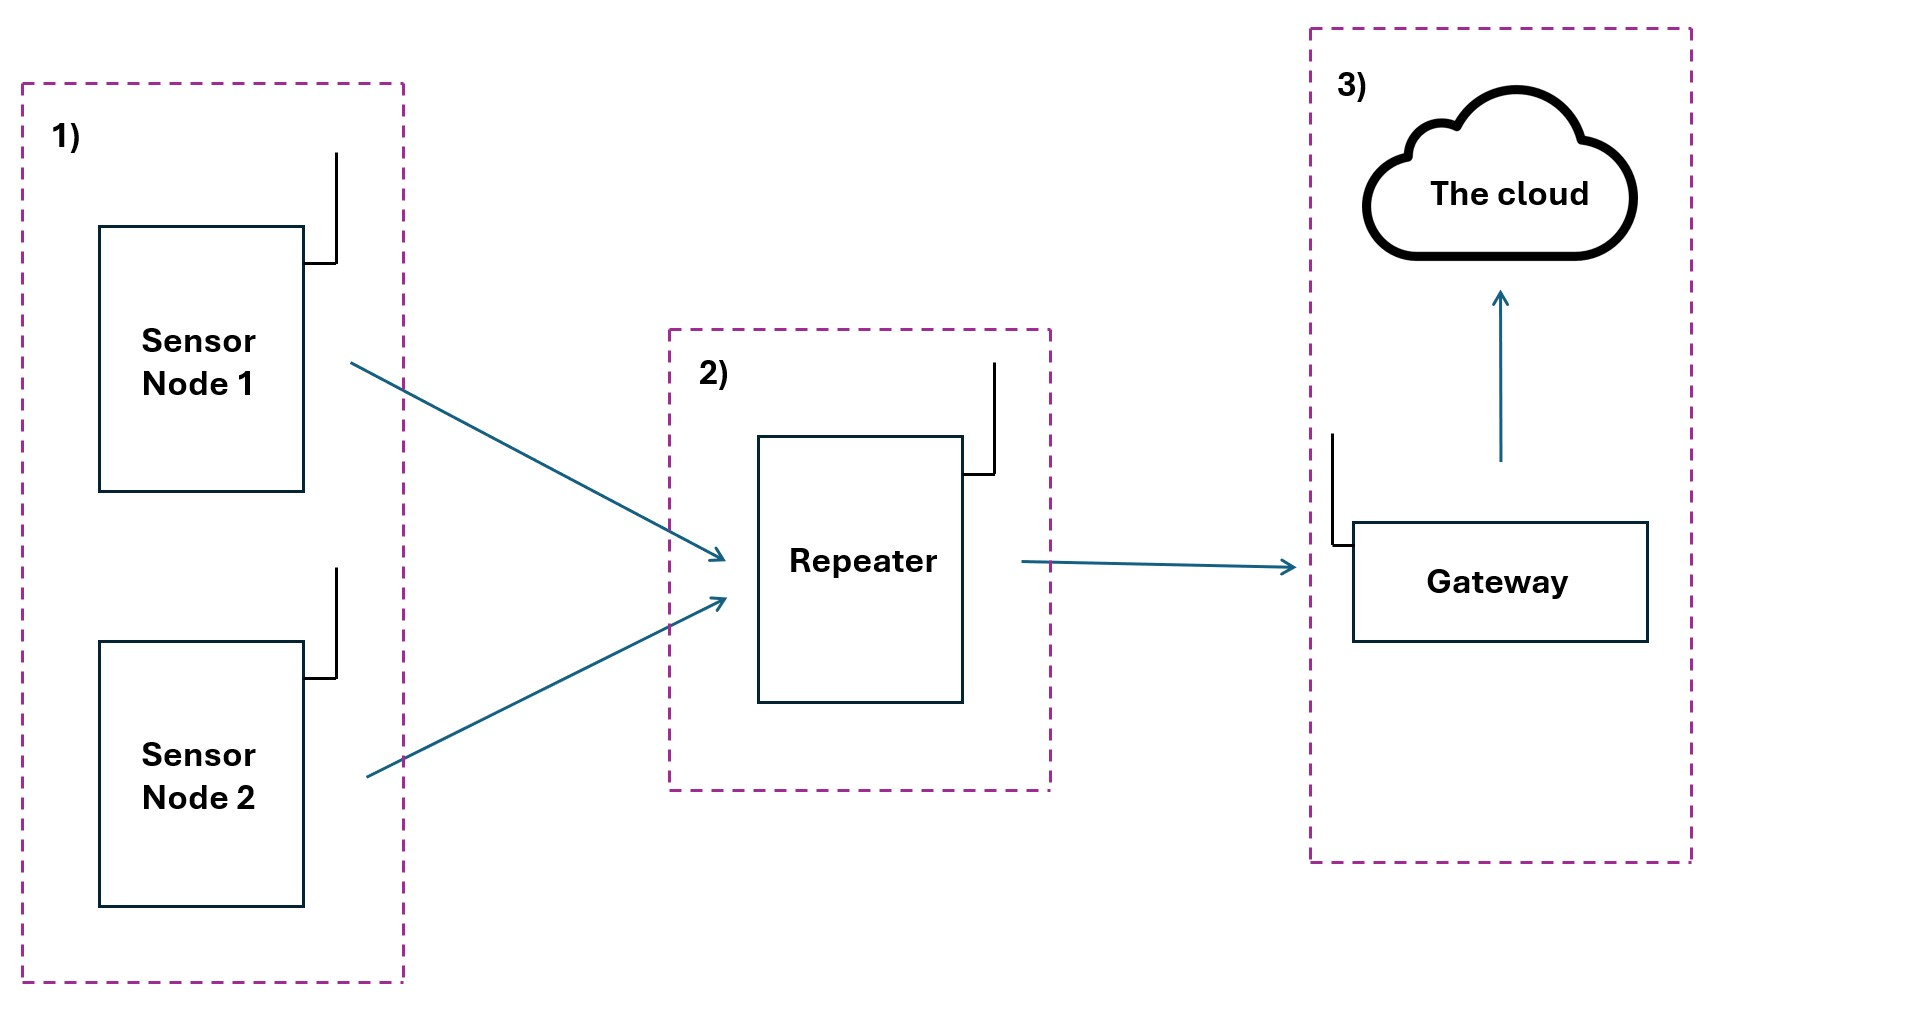
\includegraphics[width=0.9\textwidth]{contents/part-2/fig2/network-diagram.jpg}
    \caption{Network diagram of the system}
    \label{fig:network-diagram}
\end{figure}

\begin{enumerate}
    \item Sensor Node: The two nodes in this part of the network are in the
          perception layer. The nodes collect readings on temperature, humidity,
          wind speed and soil moisture levels. The results are collated into a
          comma separated string which is then emitted as a single packet from
          the LoRa transmitter.
    \item Repeater: This module is part of the network layer of the system as it
          facilitates communication between the perception layer and the
          application layer. The repeater is reads and decodes received LoRa
          signals from the sensor nodes. It then adds signal strength
          information to the string and re-emits the LoRa signal. The repeater
          has no sensors but is otherwise identical to the nodes.
    \item Gateway: The final part of the hardware system is the gateway - which
          is also part of the network layer. The gateway consists of a
          challenger to receive LoRa signals connected to a raspberry pi which
          can read the the decoded LoRa messages from the challenger's serial
          output. The raspberry pi also has a WiFi radio onboard so it is
          responsible for the uploading of data to the cloud.
\end{enumerate}





\section{Design}

\subsection{Node Components}

As the sensor nodes and the repeater are situated outside and rely on solar
power, they required components that were highly power-efficient, while also
being capable of transmitting small data packets via LoRa. An equally important
consideration for the design was how to weatherproof the final enclosure to
protect the sensitive electronics from water ingress and environmental damage.

\subsubsection{Challenger RP2040 LoRa}

The iLabs Challenger RP2040 LoRa (Figure~\ref{fig:challenger-rp2040} )is an
embedded computer that uses the Raspberry Pi RP2040 chip that was released in
2021. The RP2040 itself is a low-cost and power-efficient processor easily
capable of performing the data encoding and transmission in my use case.
Additionally, the chip is extremely popular with over 10 million units being
produced in the first two years of release \cite{pounder2023}. This popularity
means there is ample documentation for developing with this processor.

\begin{figure}[H]
    \centering
    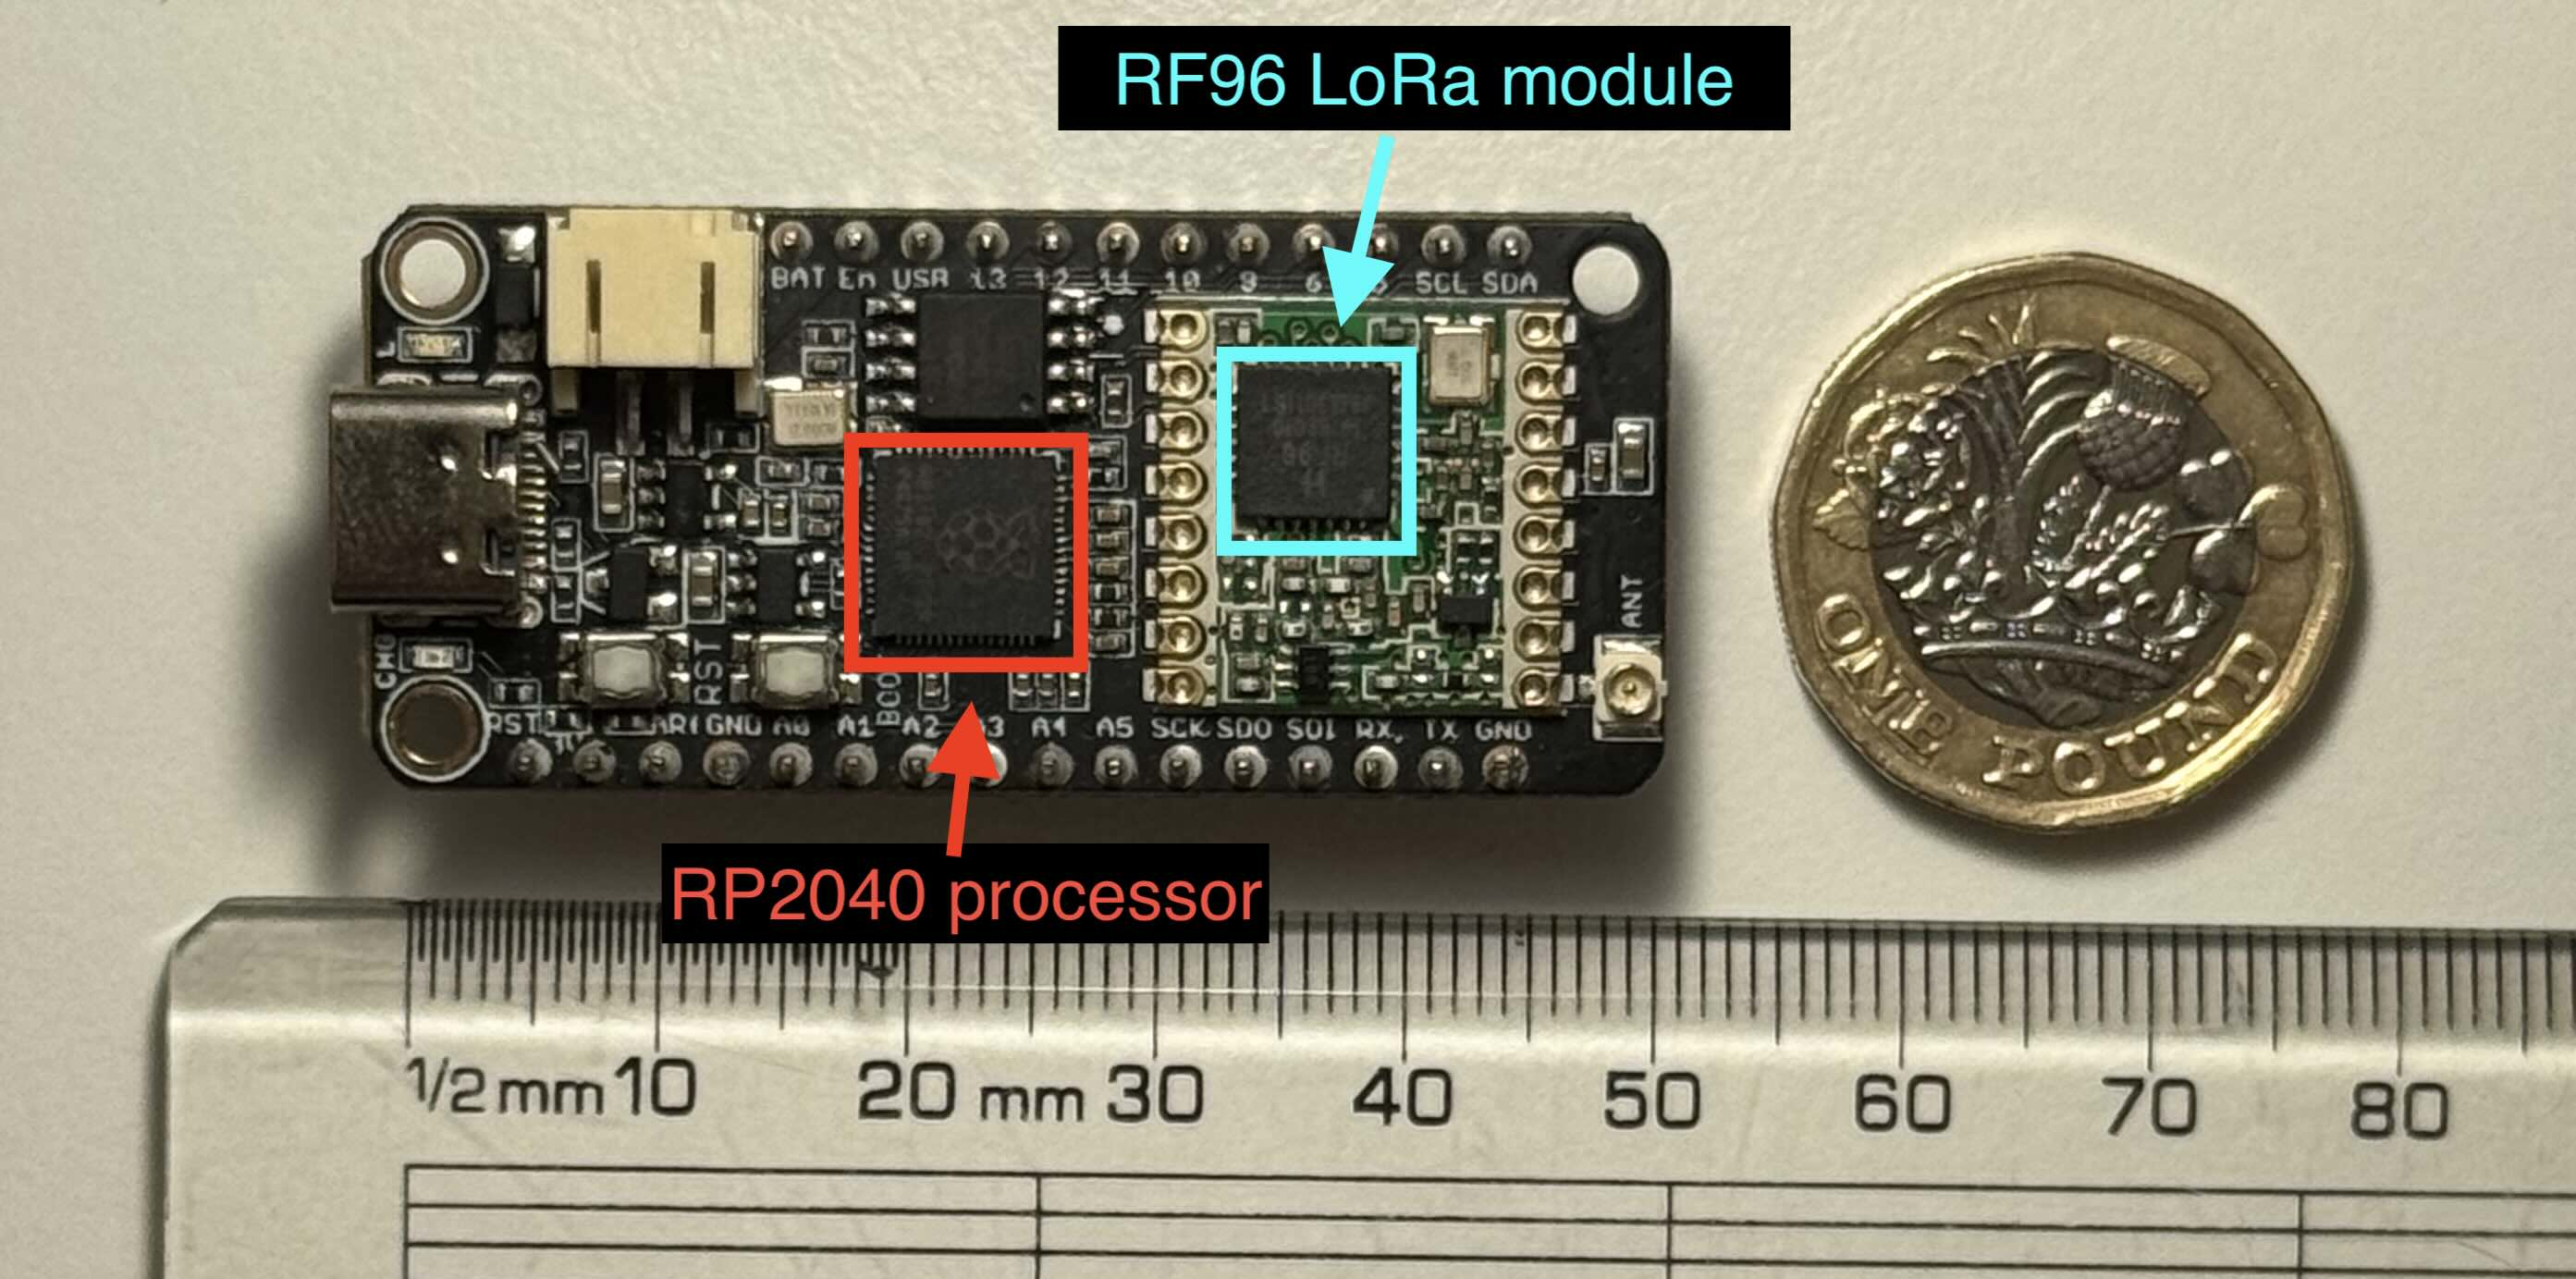
\includegraphics[width=0.8\textwidth]{contents/part-2/fig2/challenger-rp2040.jpg}
    \caption{iLabs Challenger RP2040}
    \label{fig:challenger-rp2040}
\end{figure}

The Challenger board itself is well suited for this project for several reasons.
It uses the compact Adafruit feather form factor, giving a board dimension of
just 5cm by 2cm, making it easy to mount in a small enclosure. The onboard Hope
RF96 LoRa modem is built directly into the board and the U.FL antenna connector
allows for the swapping of antenna's to different varieties. This board's LoRa
module is also set to transmit at a frequency of 868mhz which is a standard UK
frequency for LoRa and gives a good balance between range and bandwidth.

Another useful aspect of the board is the abundance of GPIO pins (20 in total)
allowing for a large number of sensors to be fitted to the board.

\subsubsection{Antennae}

The selection of antennae is one of the largest determinants of range and
reliability in the context of wireless communication systems \cite{khan2016}.
Initially I used a simple PCB antenna as shown in Figure~\ref{fig:pcb-antenna},
however as explained in the next chapter, the range of this was insufficient for
my use.

\begin{figure}[H]
    \centering
    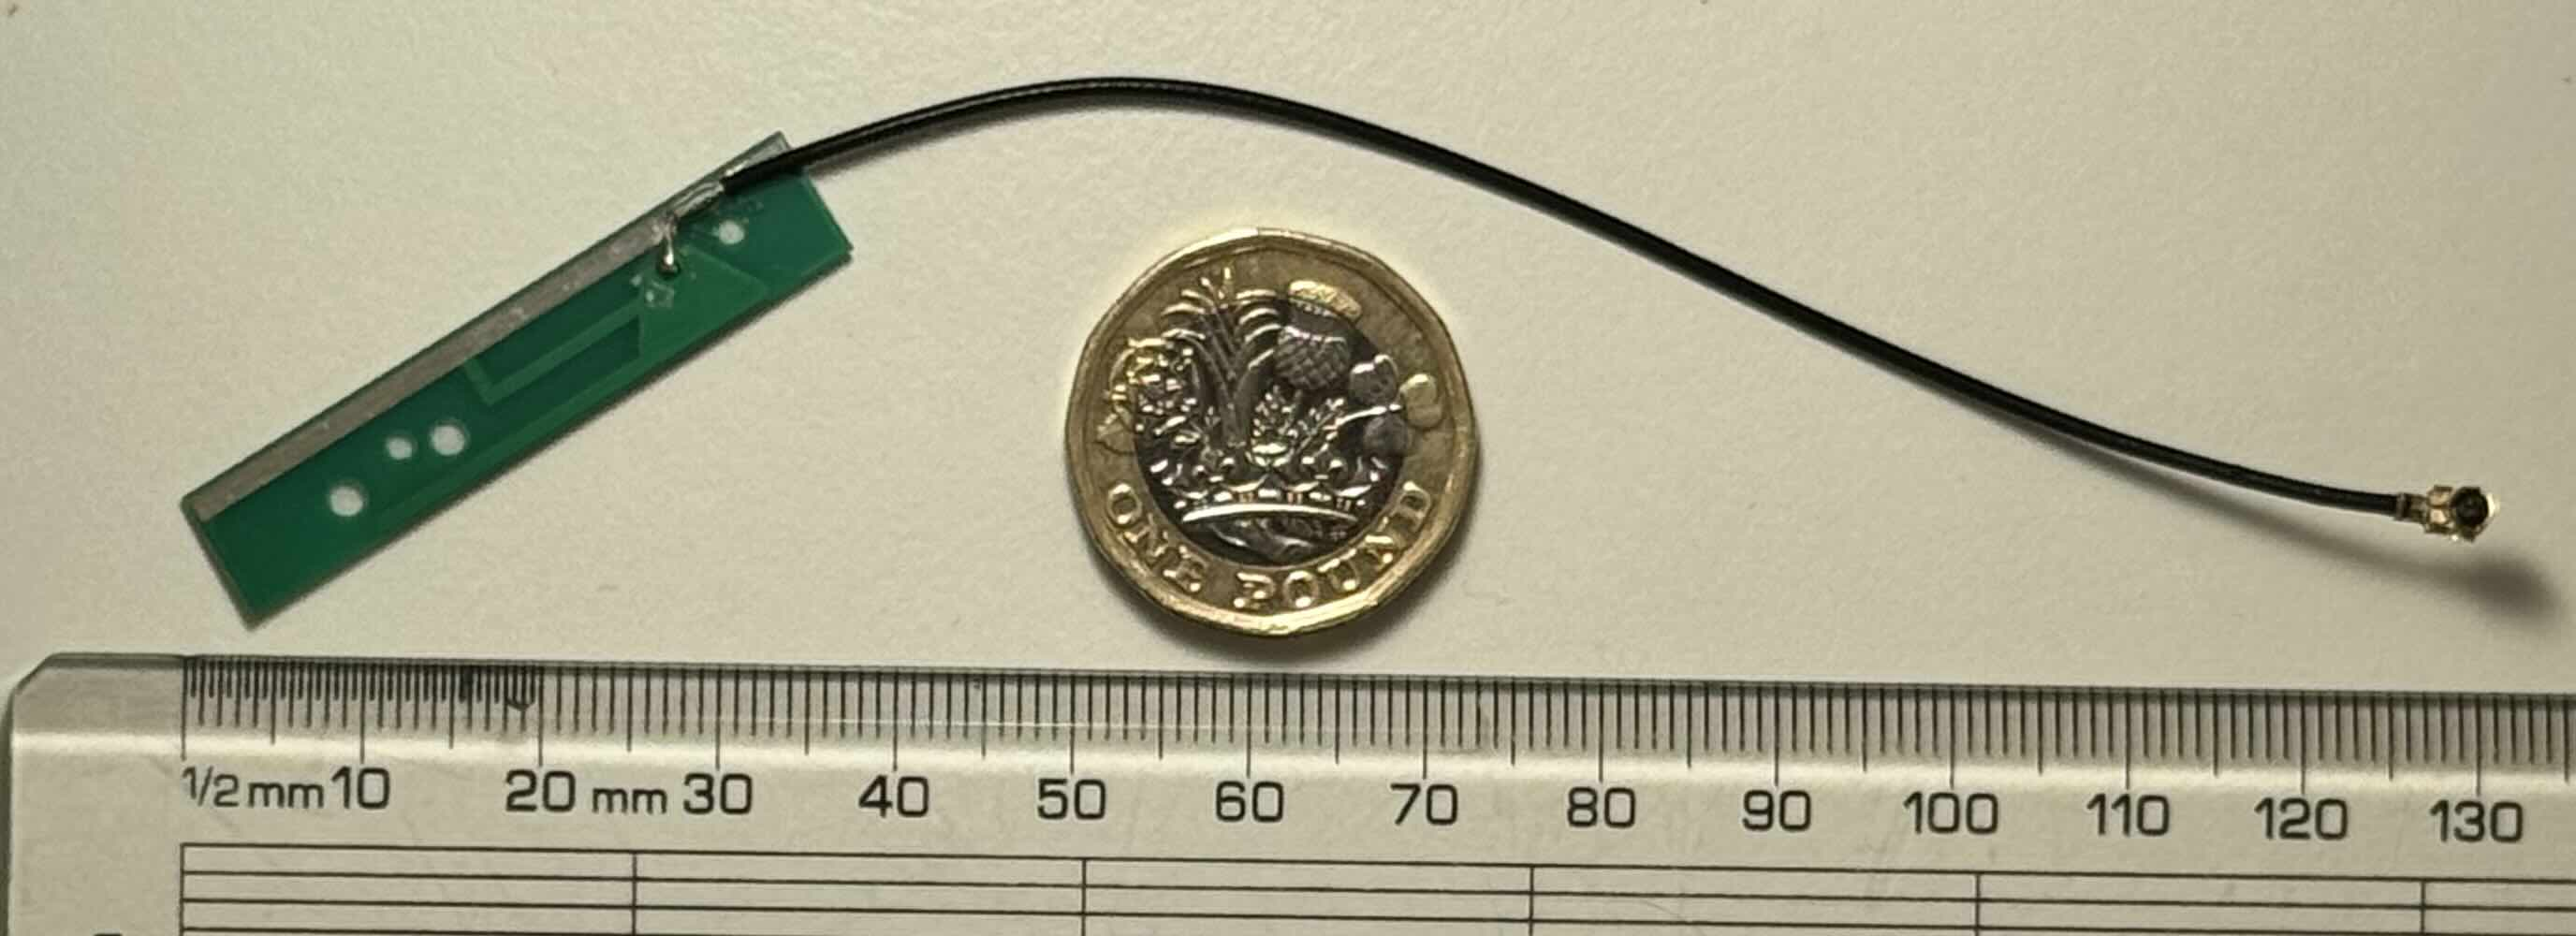
\includegraphics[width=0.8\textwidth]{contents/part-2/fig2/basic-antenna.jpg}
    \caption{Low range PCB antenna}
    \label{fig:pcb-antenna}
\end{figure}

To improve overall range I switched to a more capable omnidirectional whip
antenna that was made specifically for the Challenger RP2040. The antenna is
tuned to perform best at the 868mhz frequency range - which is the range I was
using.

\begin{figure}[H]
    \centering
    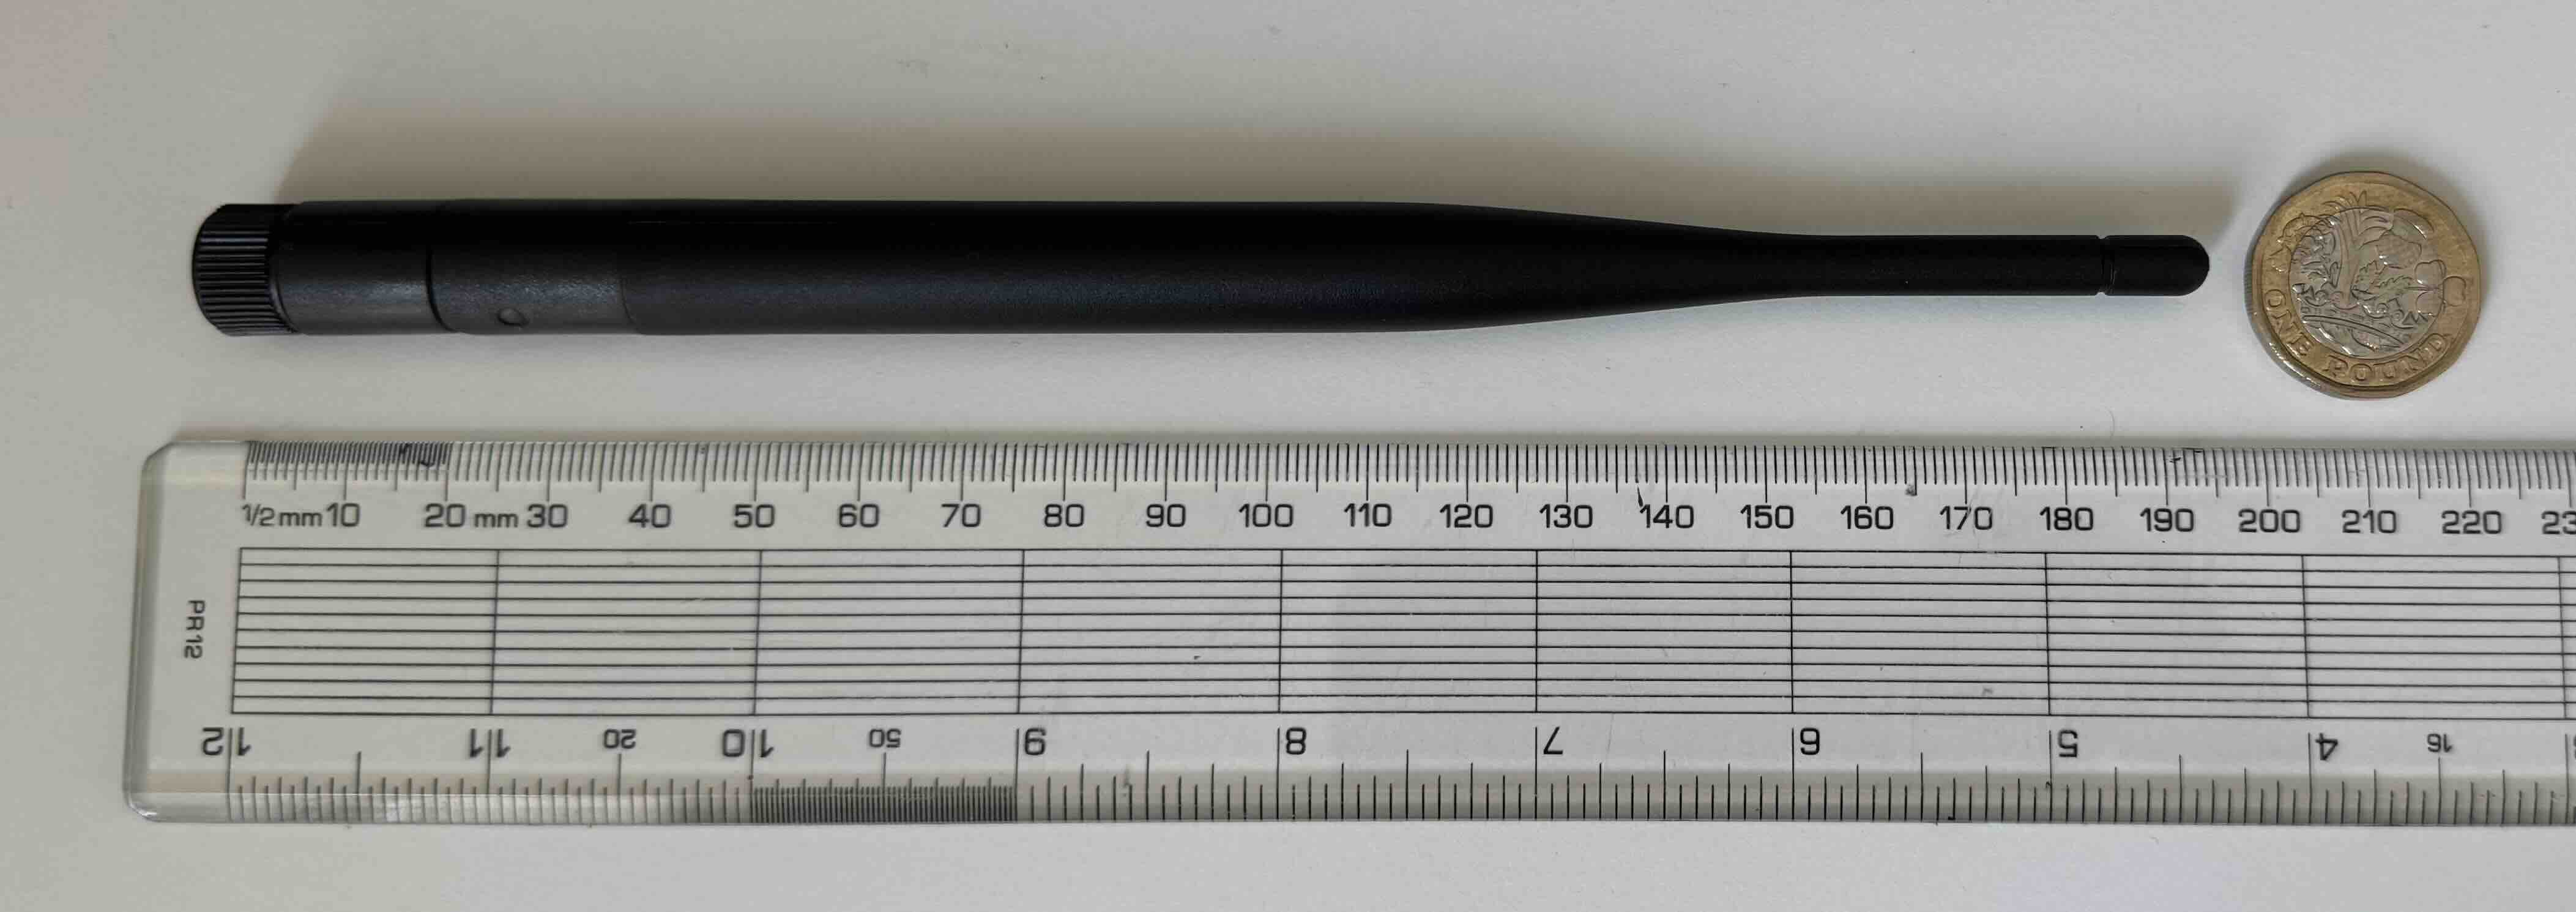
\includegraphics[width=0.8\textwidth]{contents/part-2/fig2/good-antenna.jpg}
    \caption{iLabs whip style LoRa antenna (868mhz)}
    \label{fig:good-antenna}
\end{figure}

\subsubsection{Powering the node}

To allow for continuous operation away from power sources, I attached a 6W
Monocrystalline Silicon Solar Panel (Figure~\ref{fig:solar-module})to each of
the nodes. I also installed a solar power management module
(Figure~\ref{fig:solar-module}) onto the Challengers. This module moderates the
output from the solar panels which is at too high a voltage to directly power
the nodes. It also incorporates a battery that charges from the solar panel
output and provides power to the nodes when the solar power is not available.

\begin{figure}[H]
    \centering
    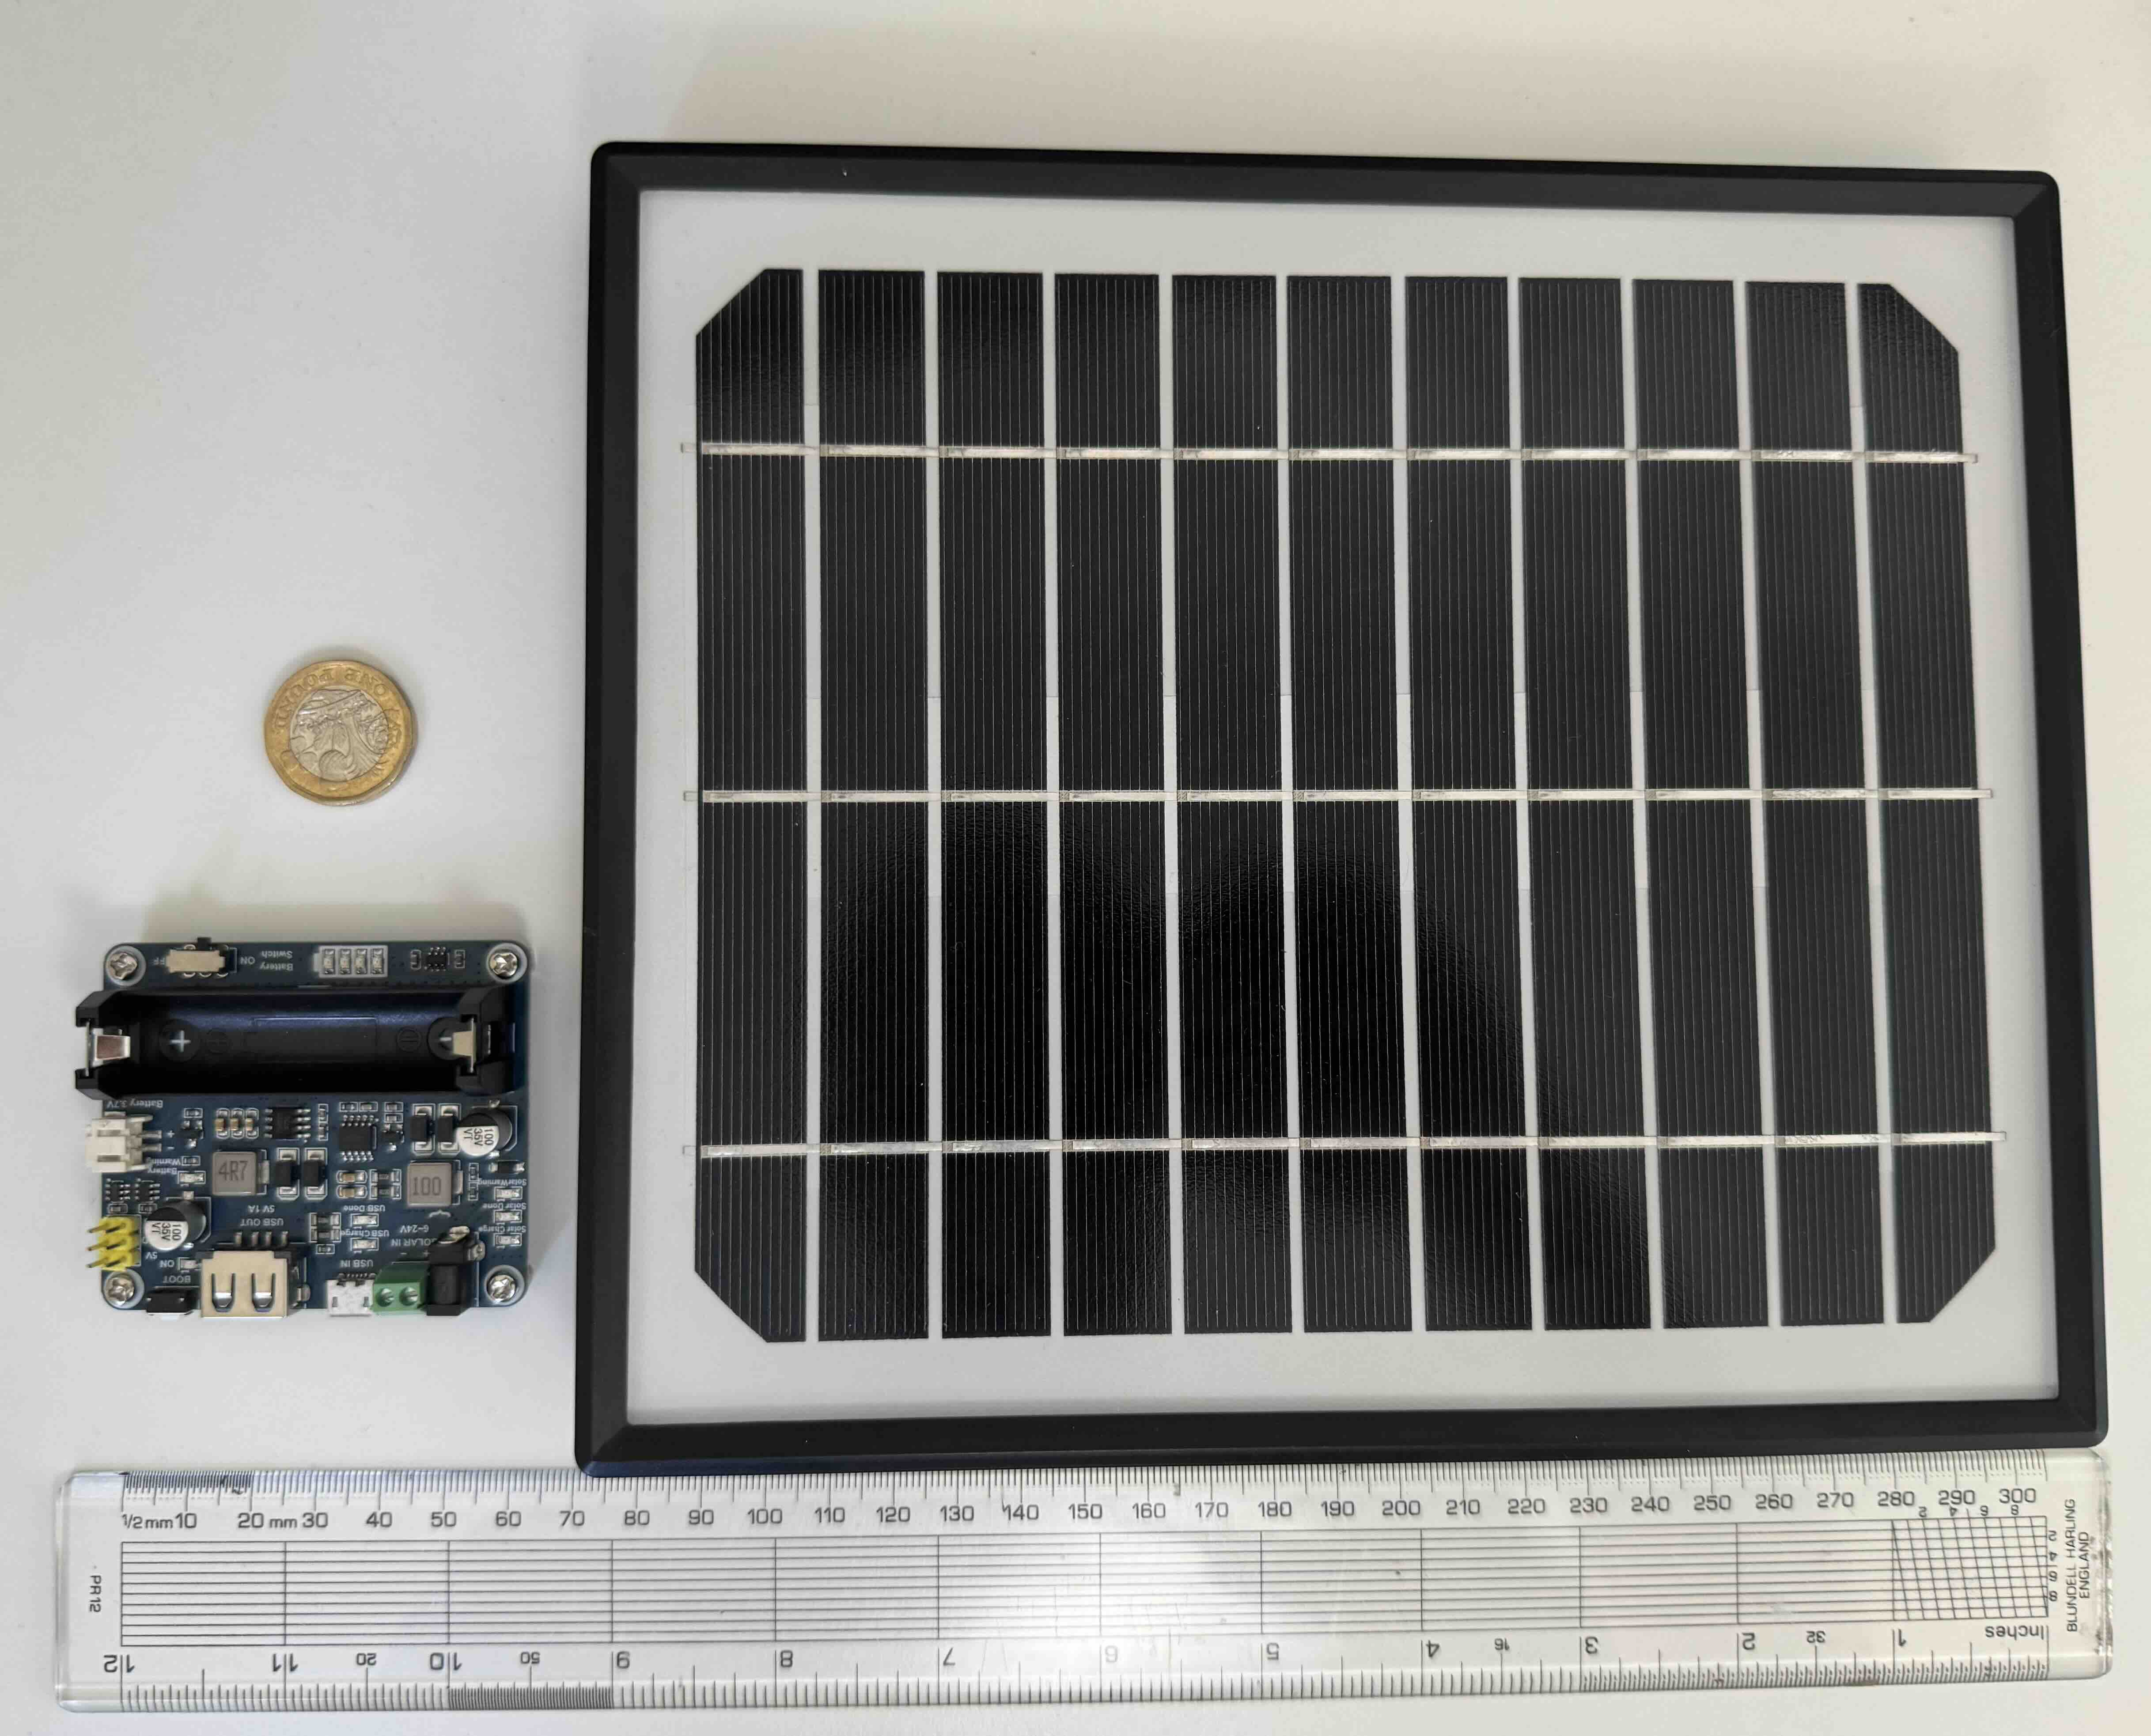
\includegraphics[width=0.5\textwidth]{contents/part-2/fig2/solar-panel-manager.jpg}
    \caption{Waveshare solar power management module (left), solar panel (right)}
    \label{fig:solar-module}
\end{figure}

\subsubsection{Sensor selection} \label{sec:sensor-selection}

\paragraph{Temperature and humidity sensor}

I used a DHT11 temperature/humidity sensor (Figure~\ref{fig:dht11}) for each
sensor node to provide basic readings. It was chosen for it's low cost,
availability and compatibility with both the RP2040 Challenger and CircuitPython
(via libraries). The sensor can be connected to the microcontroller using a
single GPIO pin as well as the usual power and ground pin.

\begin{figure}[H]
    \centering
    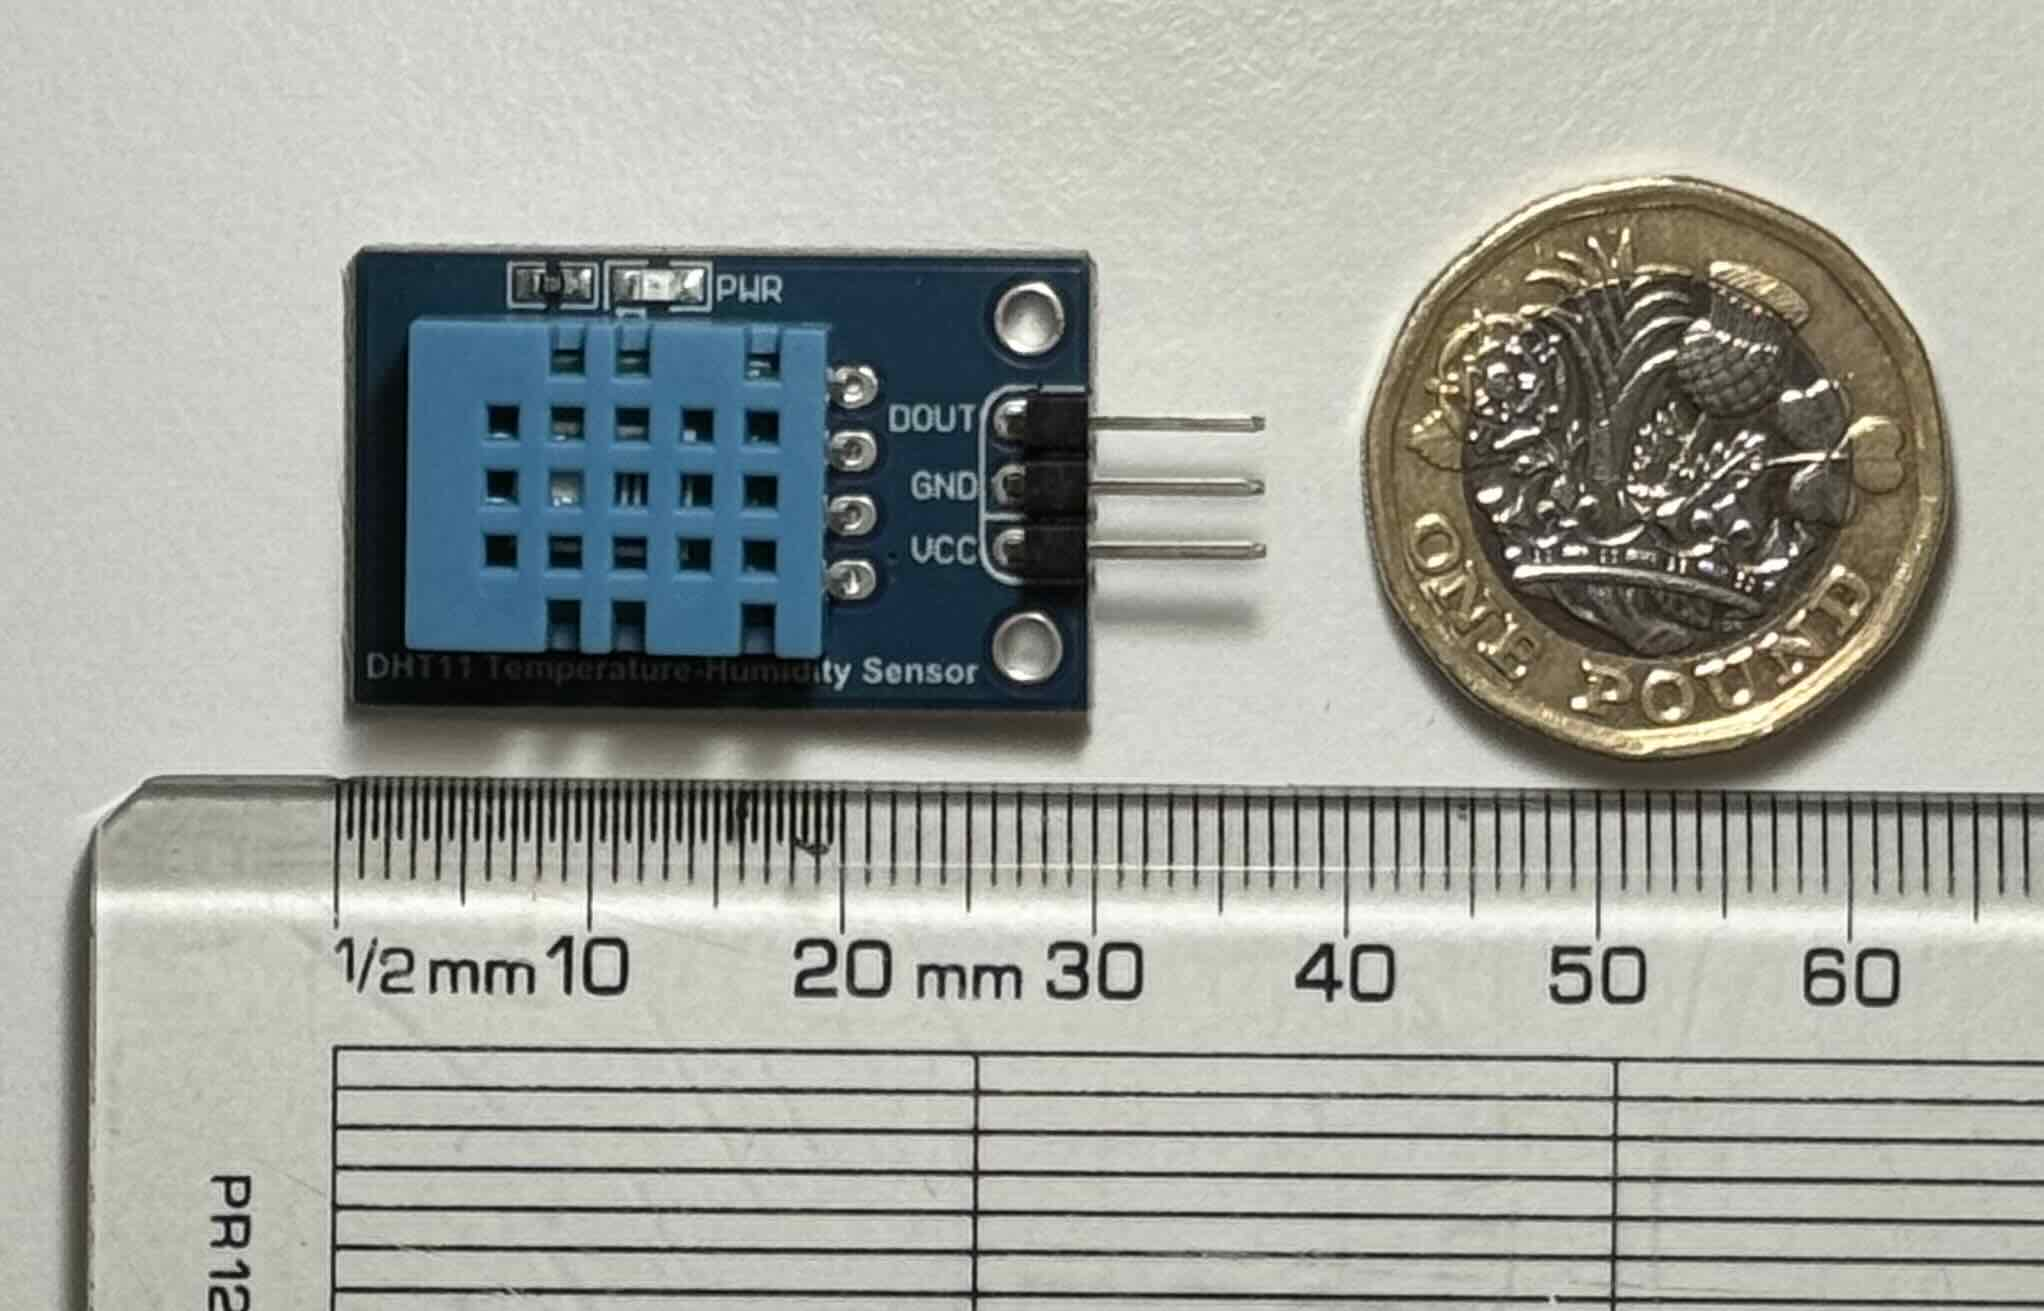
\includegraphics[width=0.7\textwidth]{contents/part-2/fig2/dht11.jpg}
    \caption{Waveshare DHT11 temperature/humidity sensor}
    \label{fig:dht11}
\end{figure}

\paragraph{Soil moisture sensor}

The main choice between soil moisture sensors is whether to use a capacitative
or resistive style sensor. In a resistance sensor the diodes must be bare plated
metal in order for resistance between each diode to be measured. However the
disadvantage of this is that bare metal corrodes in the presence of water, and
corrosion affects the accuracy of the sensor.  The benefit of capacitative
sensors is that the diodes are covered by a protective layer making them much
less susceptible to corrosion. For this reason I chose a capacitive sensor
(Figure~\ref{fig:soil-sensor}).


\begin{figure}[H]
    \centering
    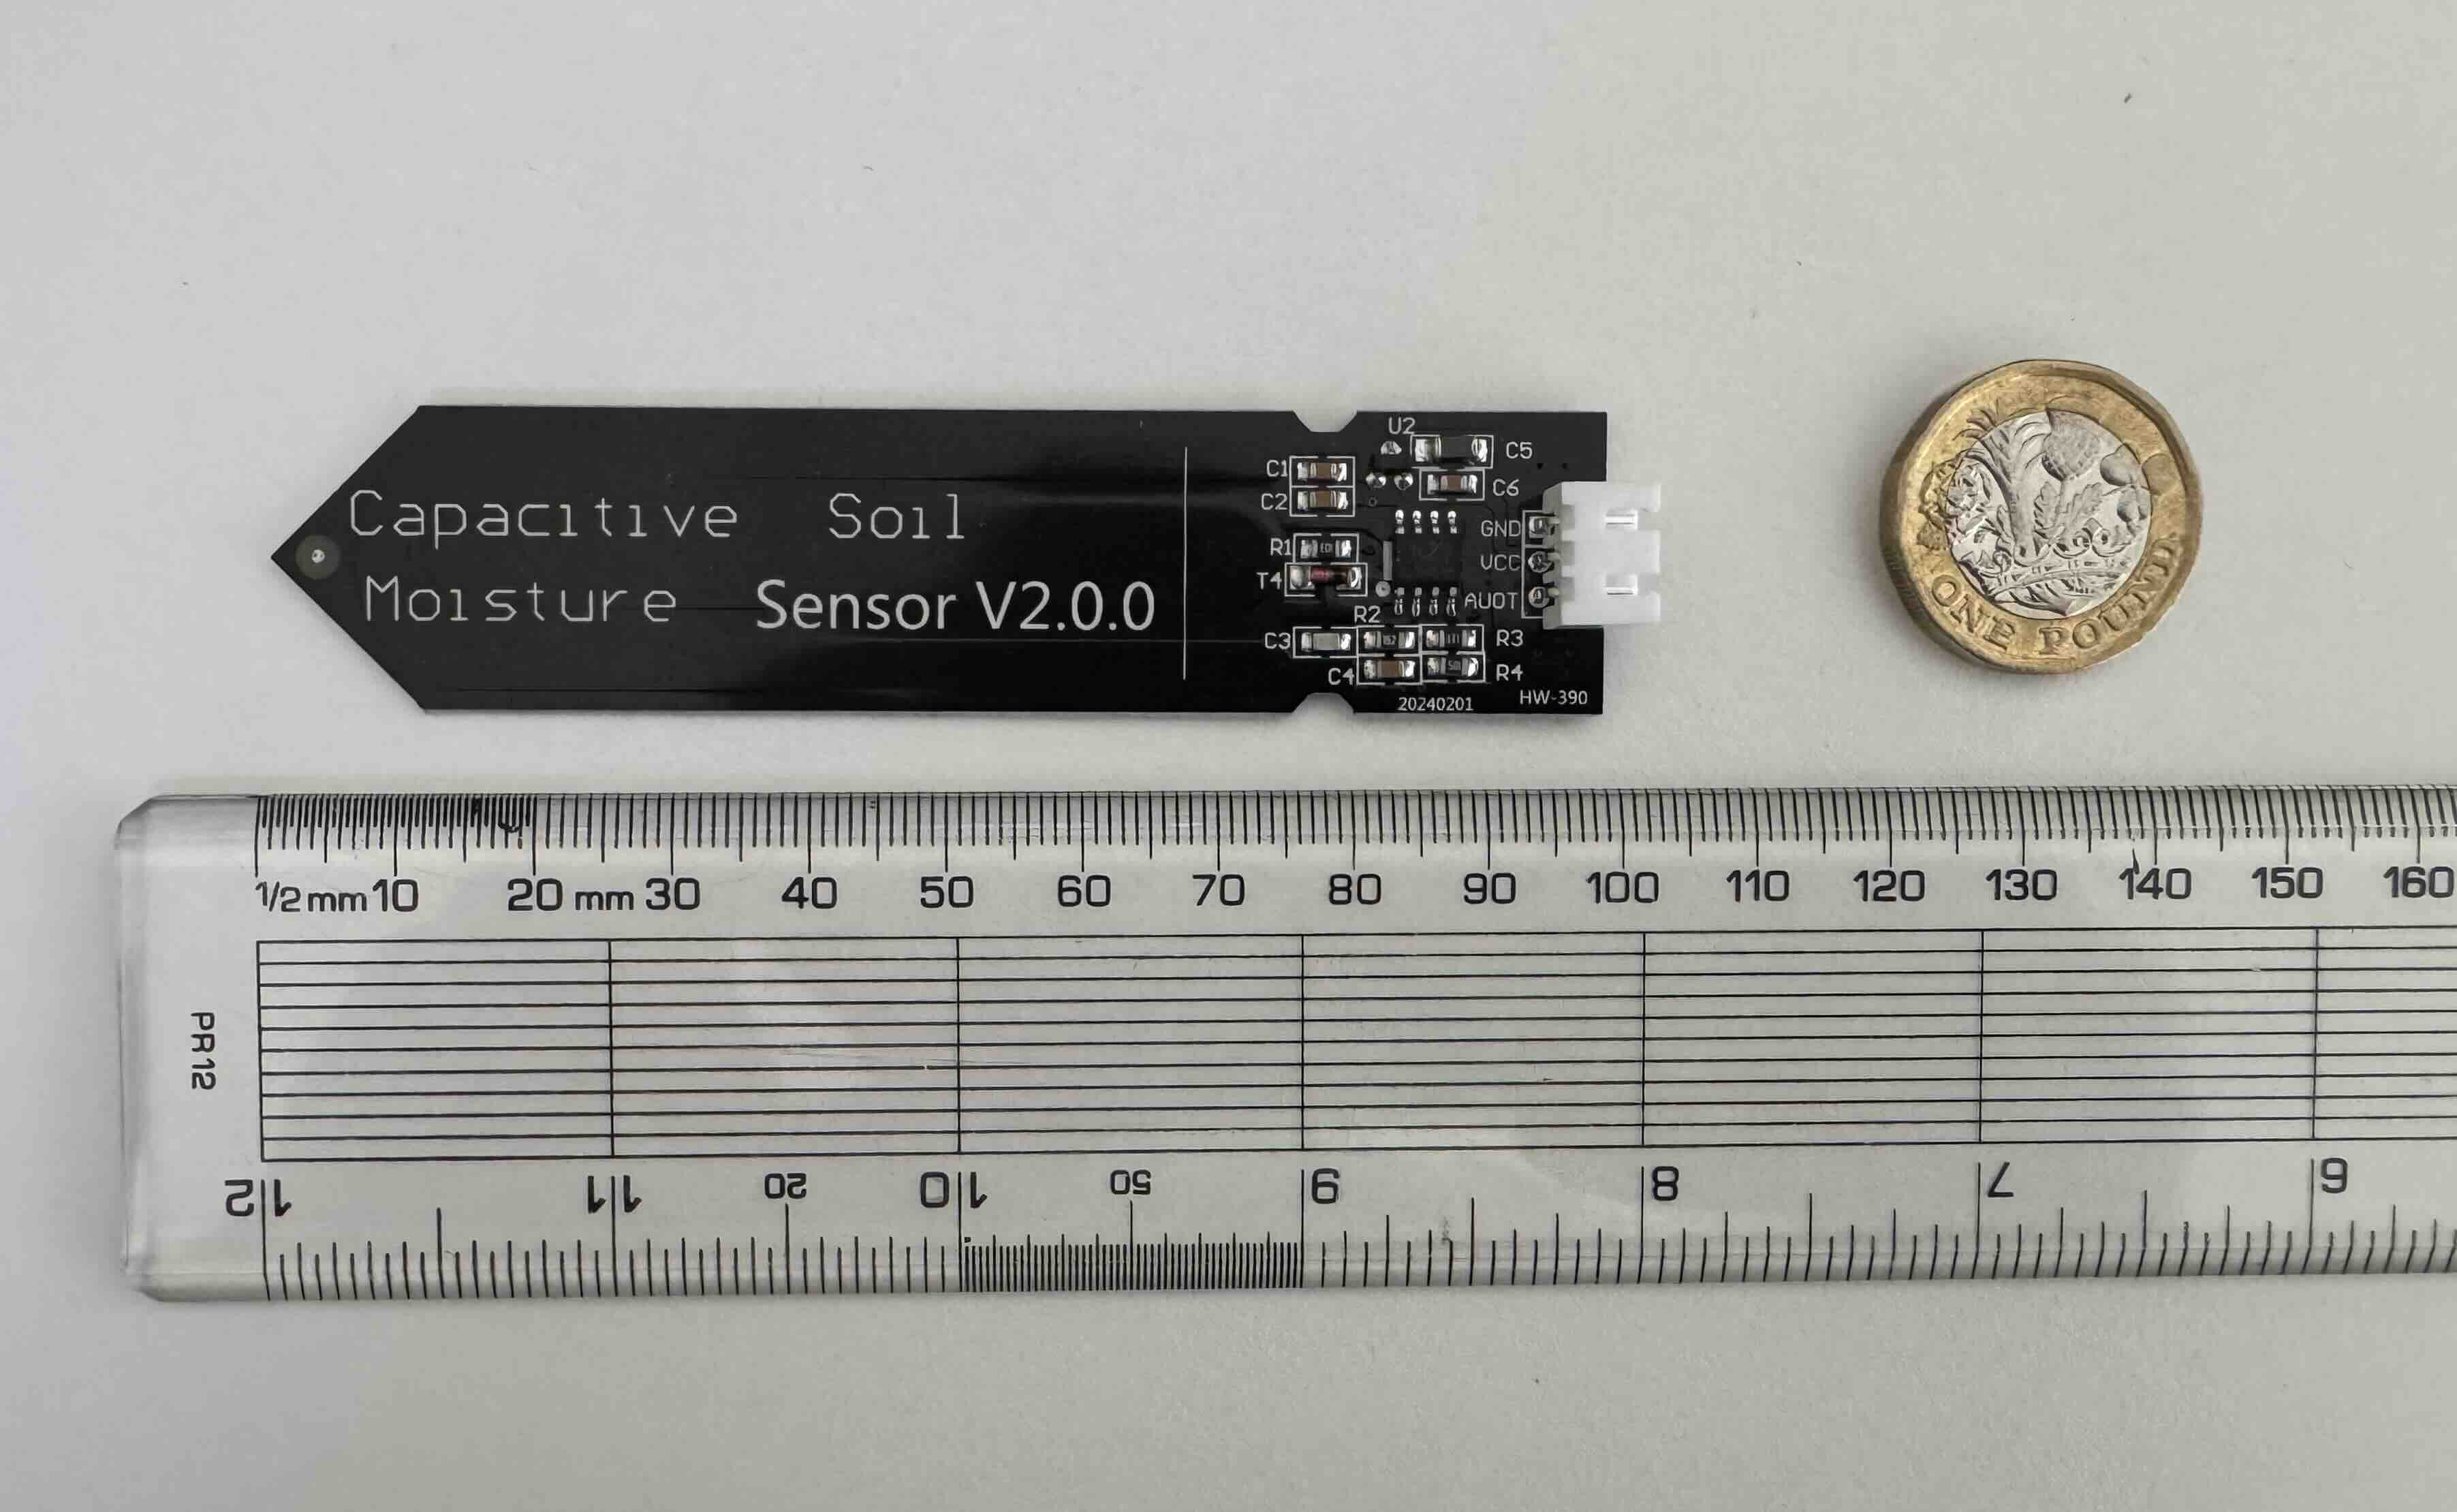
\includegraphics[width=0.7\textwidth]{contents/part-2/fig2/soil-sensor.jpg}
    \caption{The Pi Hut capacitive soil moisture sensor}
    \label{fig:soil-sensor}
\end{figure}

\paragraph{Wind speed sensor (Anemometer)}\label{sec:anemometer}

The anemometer chosen (Figure~\ref{fig:wind-sensor}) was the DFROBOT wind speed
sensor. It balances value with construction quality as unlike many other cup
style sensors this is made of metal and rated for outdoor use. When I chose this
component I was unaware that the RS485 serial communication protocol that the
sensor used was not compatible with the Challengers UART protocol. Fortunately,
I was able to purchase an RS485 to UART serial converter that allowed the
devices to communicate.

\begin{figure}[H]
    \centering
    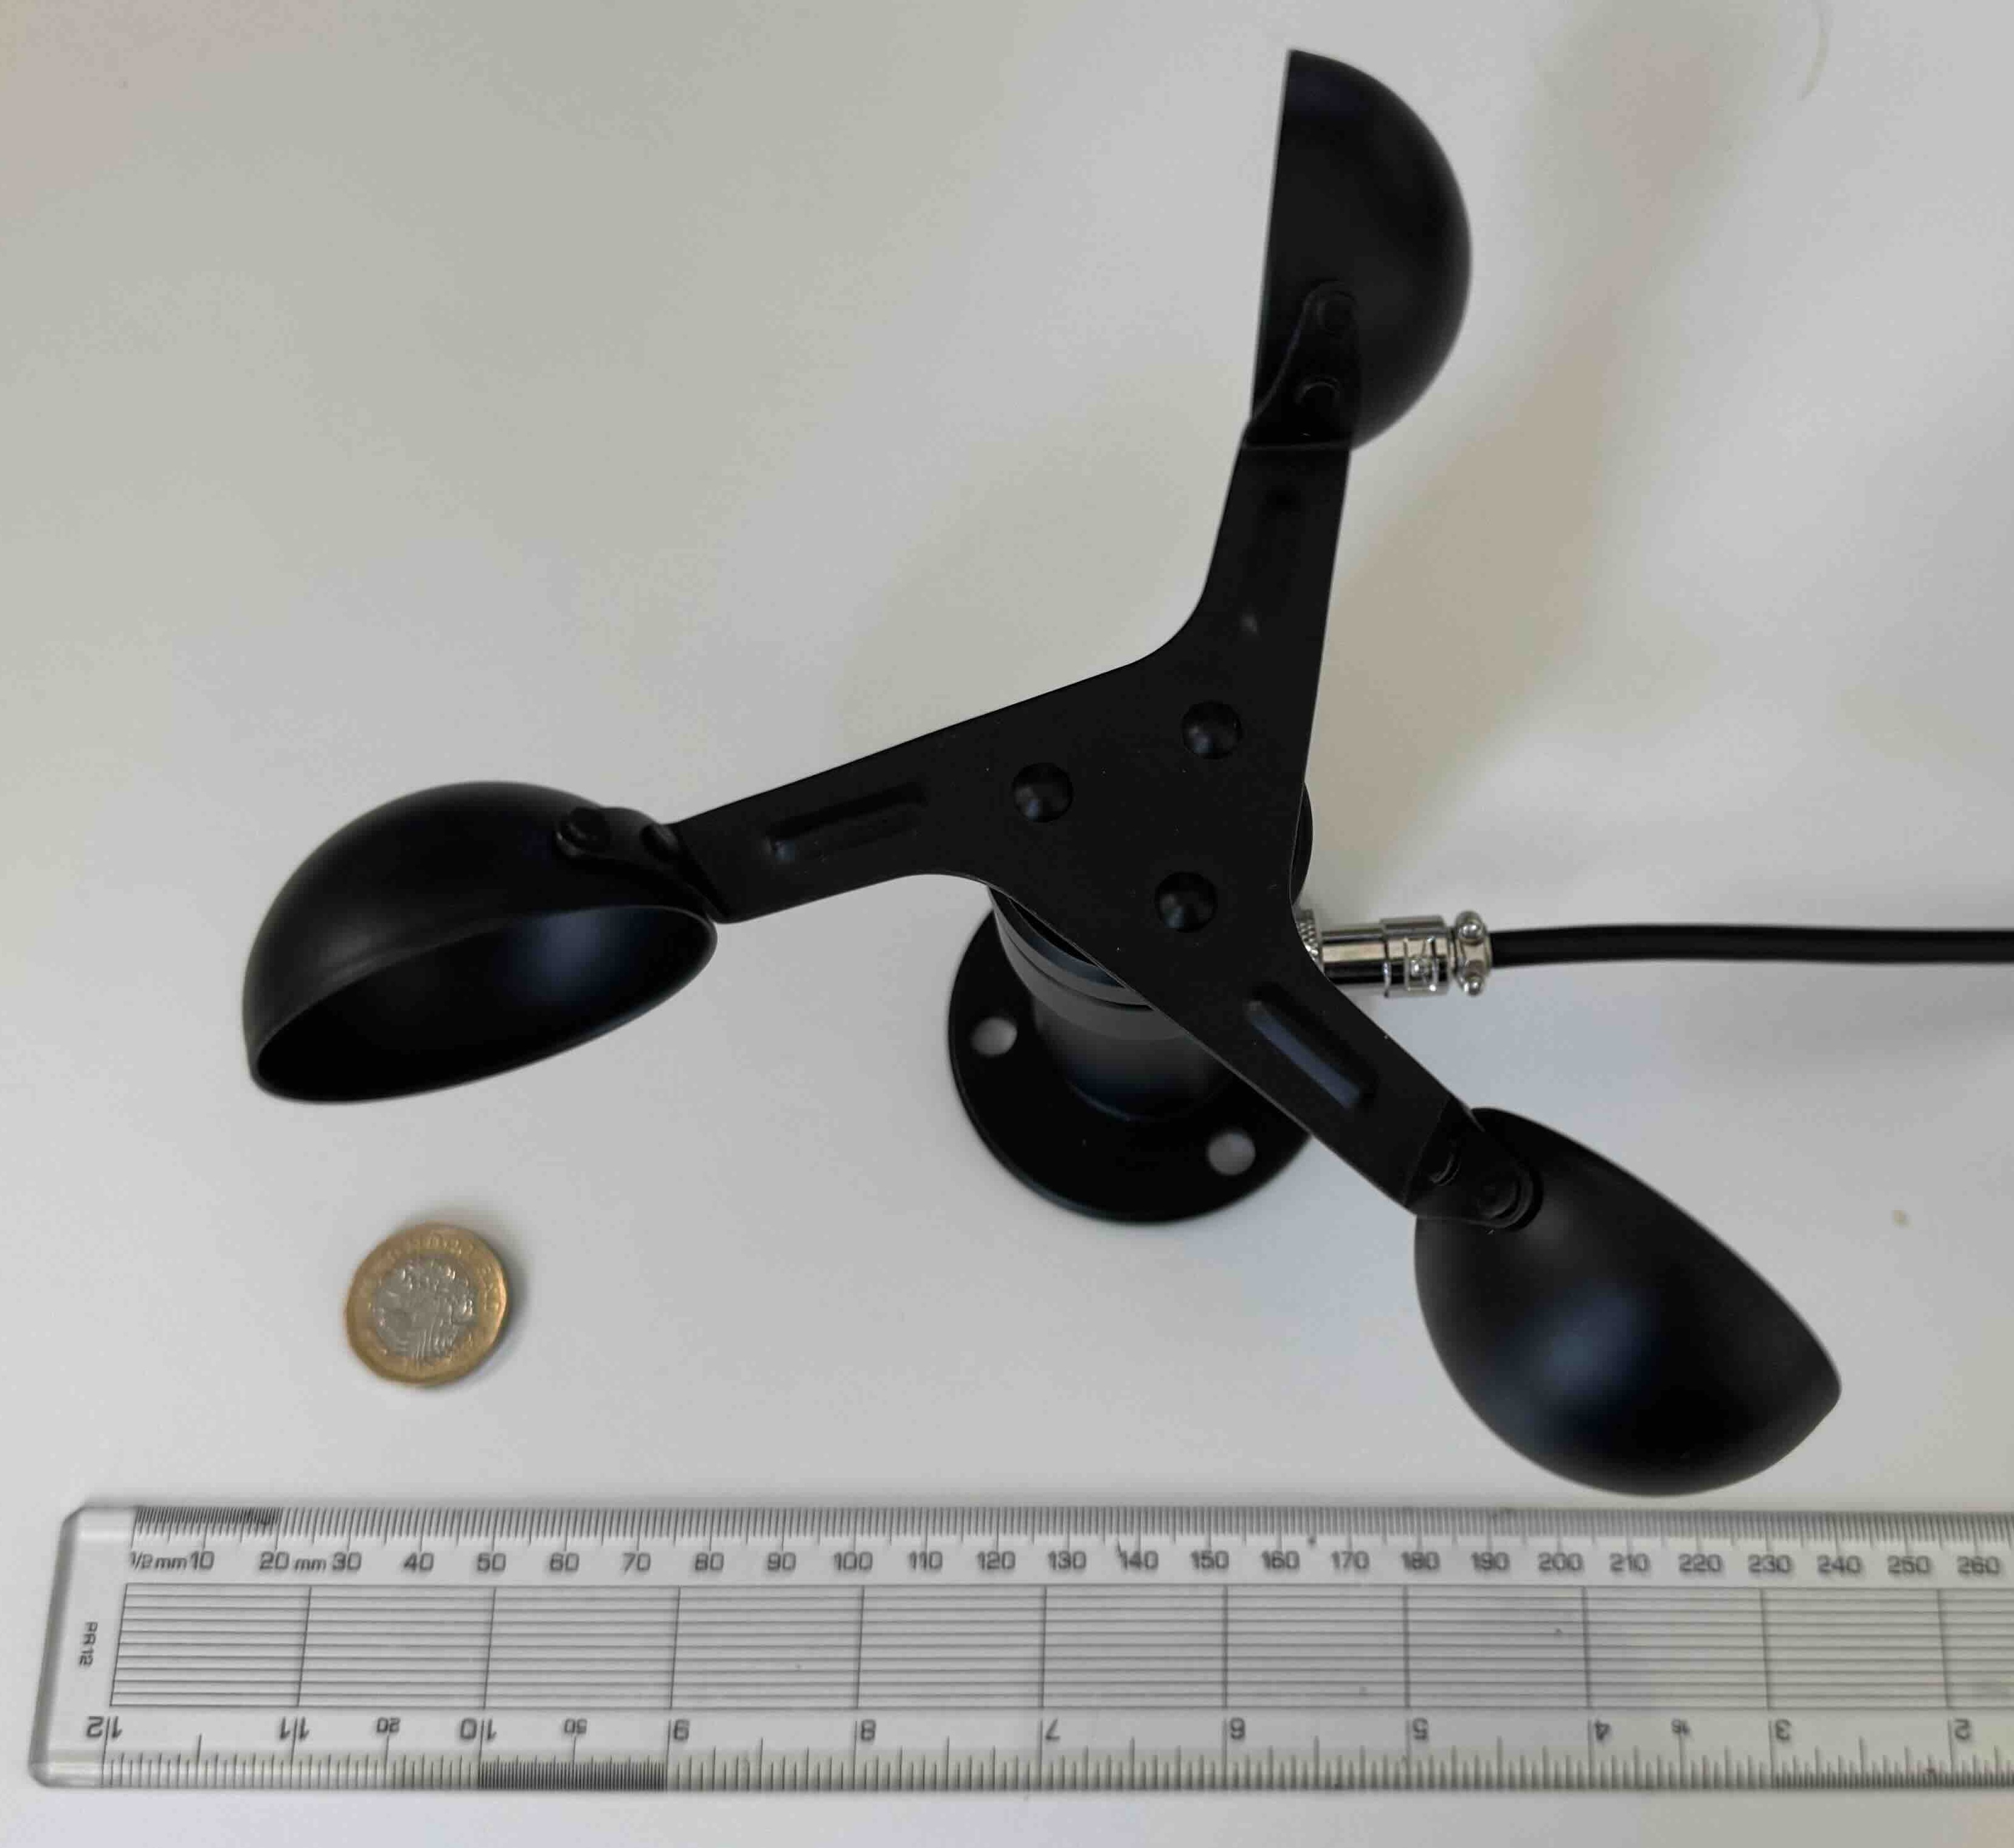
\includegraphics[width=0.5\textwidth]{contents/part-2/fig2/wind-sensor.jpg}
    \caption{DFROBOT wind speed sensor}
    \label{fig:wind-sensor}
\end{figure}

A second issue was that the anemometer needed a 7V-24V input voltage to take
readings while the maximum voltage the Challenger can provide was 5V. To remedy
this I bought a 9V step up converter to boost the Challenger's voltage to the
required level.

\subsection{Gateway}

The components of the gateway consisted of a Challenger RP2040 with a whip
antenna. The board was connected to a Raspberry Pi 5 with 8GB of memory and an
onboard Wi-Fi radio. (Figure~\ref{fig:raspberry-pi}). This Raspberry Pi was
significantly more powerful than was needed but it was already available from
the university for use for this project. The Challenger receives and decodes
messages from the repeater. The Raspberry Pi reads the decoded LoRa message from
the serial output and then sends a POST response to the backend API which
inserts the data into a SQL database.

\begin{figure}[H]
    \centering
    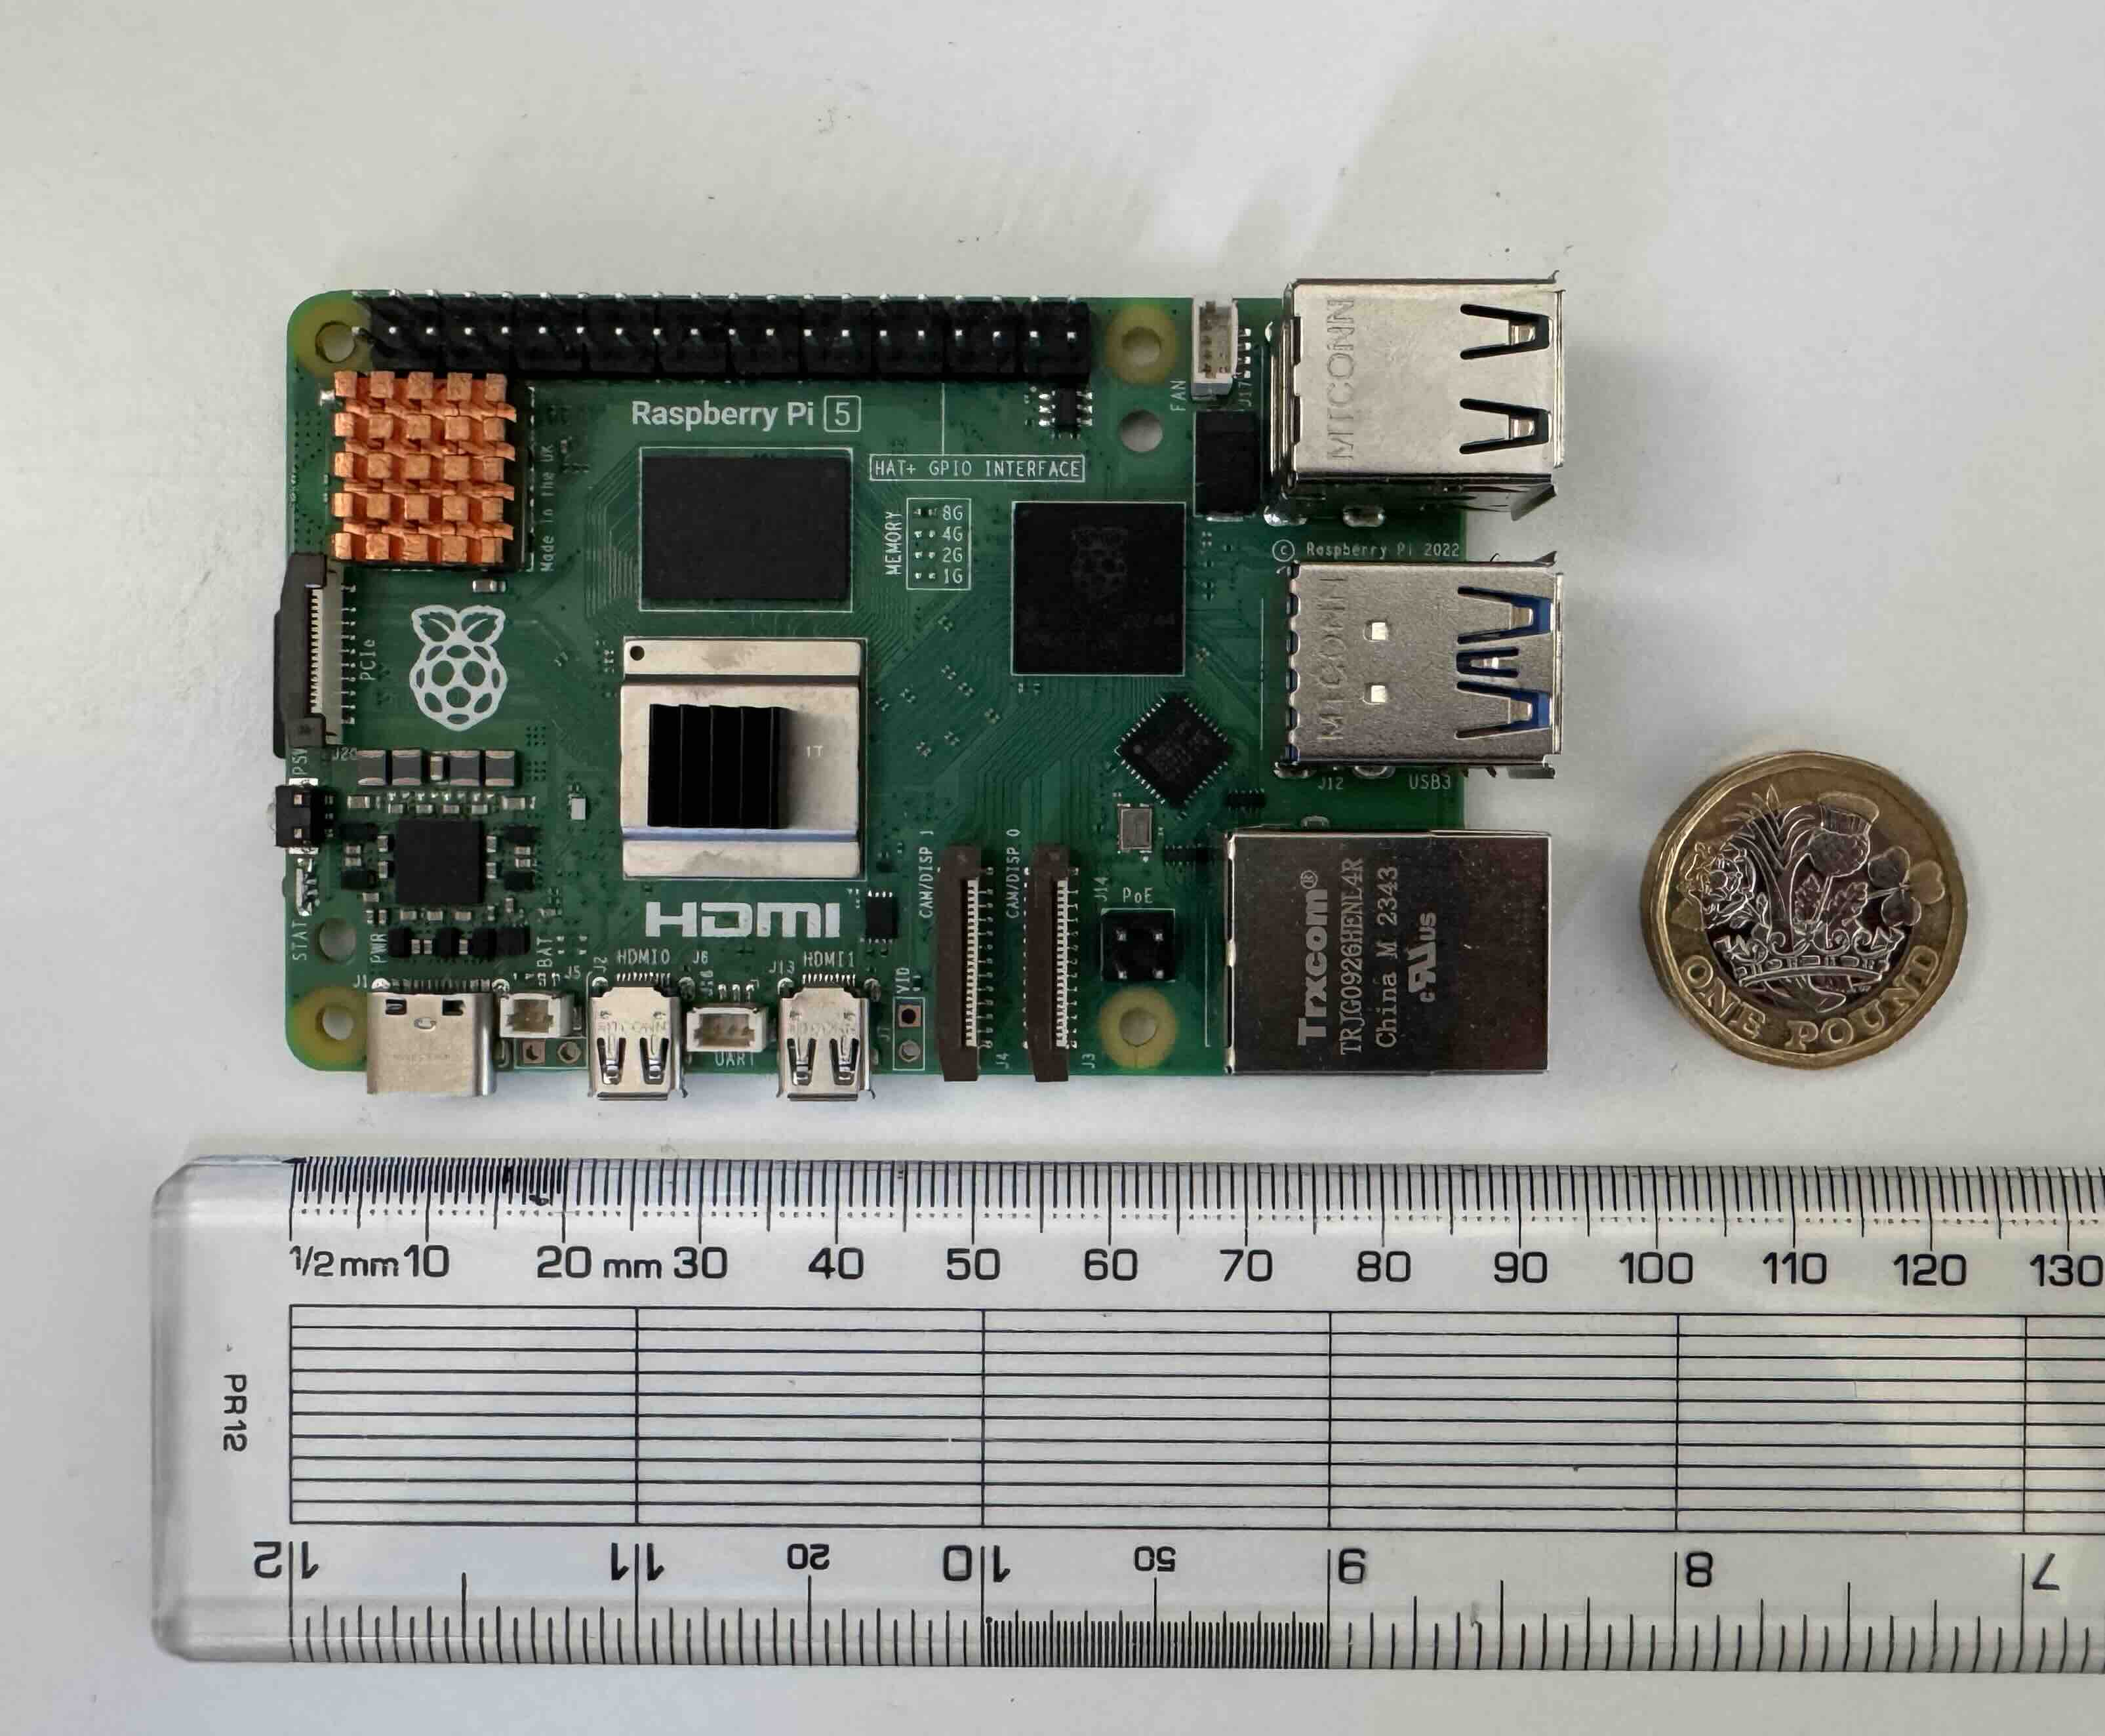
\includegraphics[width=0.4\textwidth]{contents/part-2/fig2/raspberry-pi.jpg}
    \caption{Raspberry Pi 5 (8GB)}
    \label{fig:raspberry-pi}
\end{figure}



\section{Development and testing}

\subsection{Range tests}\label{sec:range-tests}

One of the most important tasks to carry out prior to deployment in the field
was testing the range of the devices.

For this experiment I took four Challenger RP2040s to The Downs, a large public
park in Bristol. Here I tested four different antenna configurations to compare
how well the signal travelled across an increasing distance. Signal strength can
be measured using the received signal strength index (RSSI), a measure of the
difference in signal from the transmitter to the receiver and measured in
decibels.

For the test, two Challengers were programmed as transmitters, sending an
example data packet similar to the data that would be generated by the sensor
nodes. One of the transmitters used a simple PCB antenna
(Figure~\ref{fig:pcb-antenna}) while the other used a higher range whip style
antenna (Figure~\ref{fig:good-antenna}). Then I programmed the remaining two
Challengers as receivers with one using a low range antenna and the other a long
range one.

This meant that four different antenna configurations could be tested
concurrently, as the receivers could pick up the signal from each transmitter.
Before performing the test I estimated that the maximum range of each
configuration would look like the below:

\begin{enumerate}
    \item Whip antenna to whip antenna (Likely best result)
    \item PCB antenna to whip antenna
    \item Whip antenna to PCB antenna
    \item PCB antenna to PCB antenna (Likely poorest result)
\end{enumerate}

The reason I predicted the PCB transmitter to whip receiver would outperform the
whip to PCB configuration is that improving receiver sensitivity (i.e. the
ability of the receiver to 'hear') is more efficient than increasing the
transmitters effective radiated power (how loud it shouts) \cite{simpulse25}.

Nine different distances from transmitter to receiver were tested, in 200m
increments starting from 0m as a baseline to a distance of 1600m
(Figure~\ref{fig:range-test-markers}). An important aspect in getting a
successful LoRa connection is whether there is line of sight between the
transmitter and receiver. Figure~\ref{fig:range-test-elevation} shows the
elevation profile of the test area, with the initial large dip being an
inaccuracy from google earth's topology data as the 0m point is near a cliff
edge. The lowest elevation point is at the starting point at around 83m above
sea level, while the highest point was at the 1km mark at around 94m making an
elevation range of 11m. My hypothesis was that signal would likely drop off or
stop entirely beyond this point as points beyond 1000m would be below the hill
line. This would effectively mean that the receivers would be in a signal shadow
point where the transmission waves would not be able to reach them. The only
possibility for signal to reach this area would be from reflections either from
nearby buildings or topology. The effects of reflections are virtually
impossible to account for in the real world and therefore no accurate
predictions could be made.

\begin{figure}[H]
    \centering
    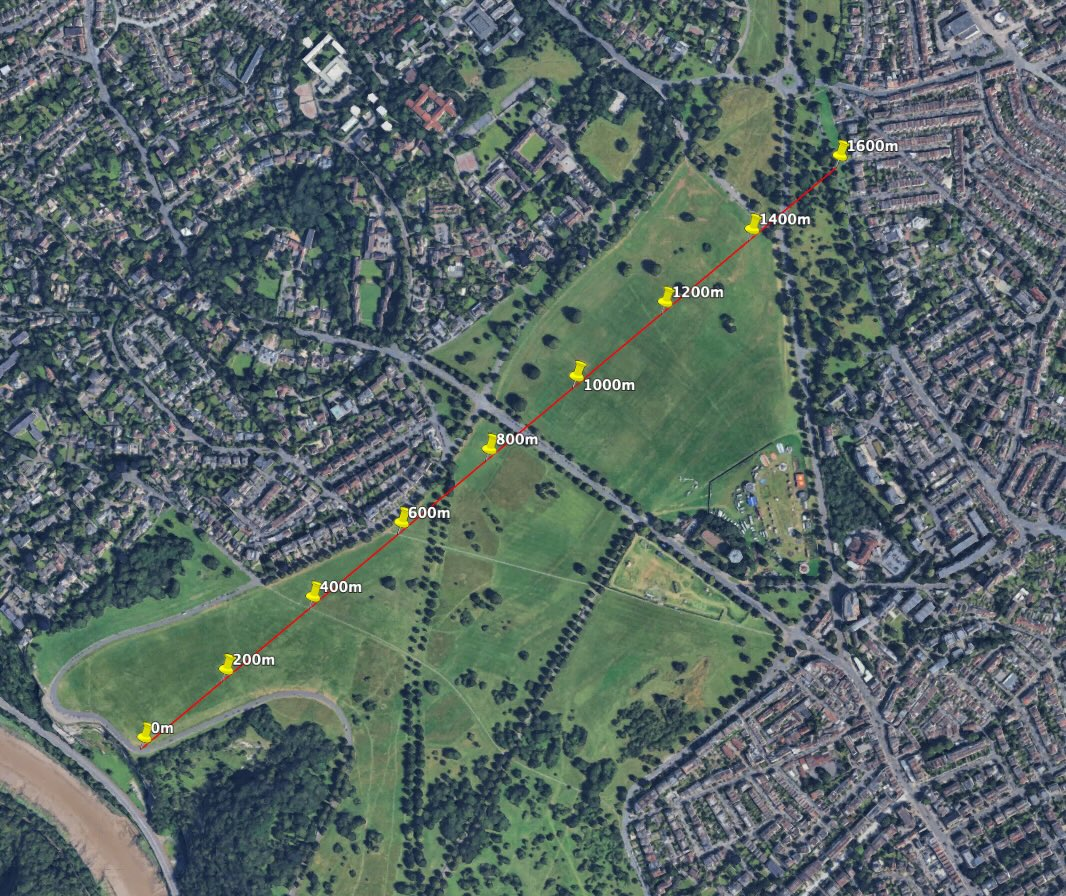
\includegraphics[width=0.7\textwidth]{contents/part-2/fig2/range-test-markers.jpg}
    \caption{Google earth image of data collection points}
    \label{fig:range-test-markers}
\end{figure}


\begin{figure}[H]
    \centering
    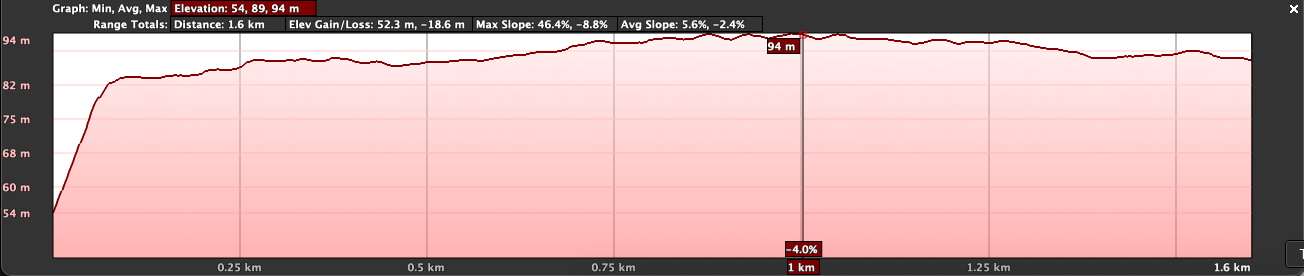
\includegraphics[width=1\textwidth]{contents/part-2/fig2/range-test-elevation-profile.jpg}
    \caption{Elevation profile of test area (ignore large dip at start)}
    \label{fig:range-test-elevation}
\end{figure}

Unfortunately, at the time of the test a festival was being run between the
1200m and 1400m mark. The festival had a number of large tents and temporary
buildings constructed which very likely negatively affected the signal. Final
data for the range test is shown below.

\begin{figure}[H]
    \centering
    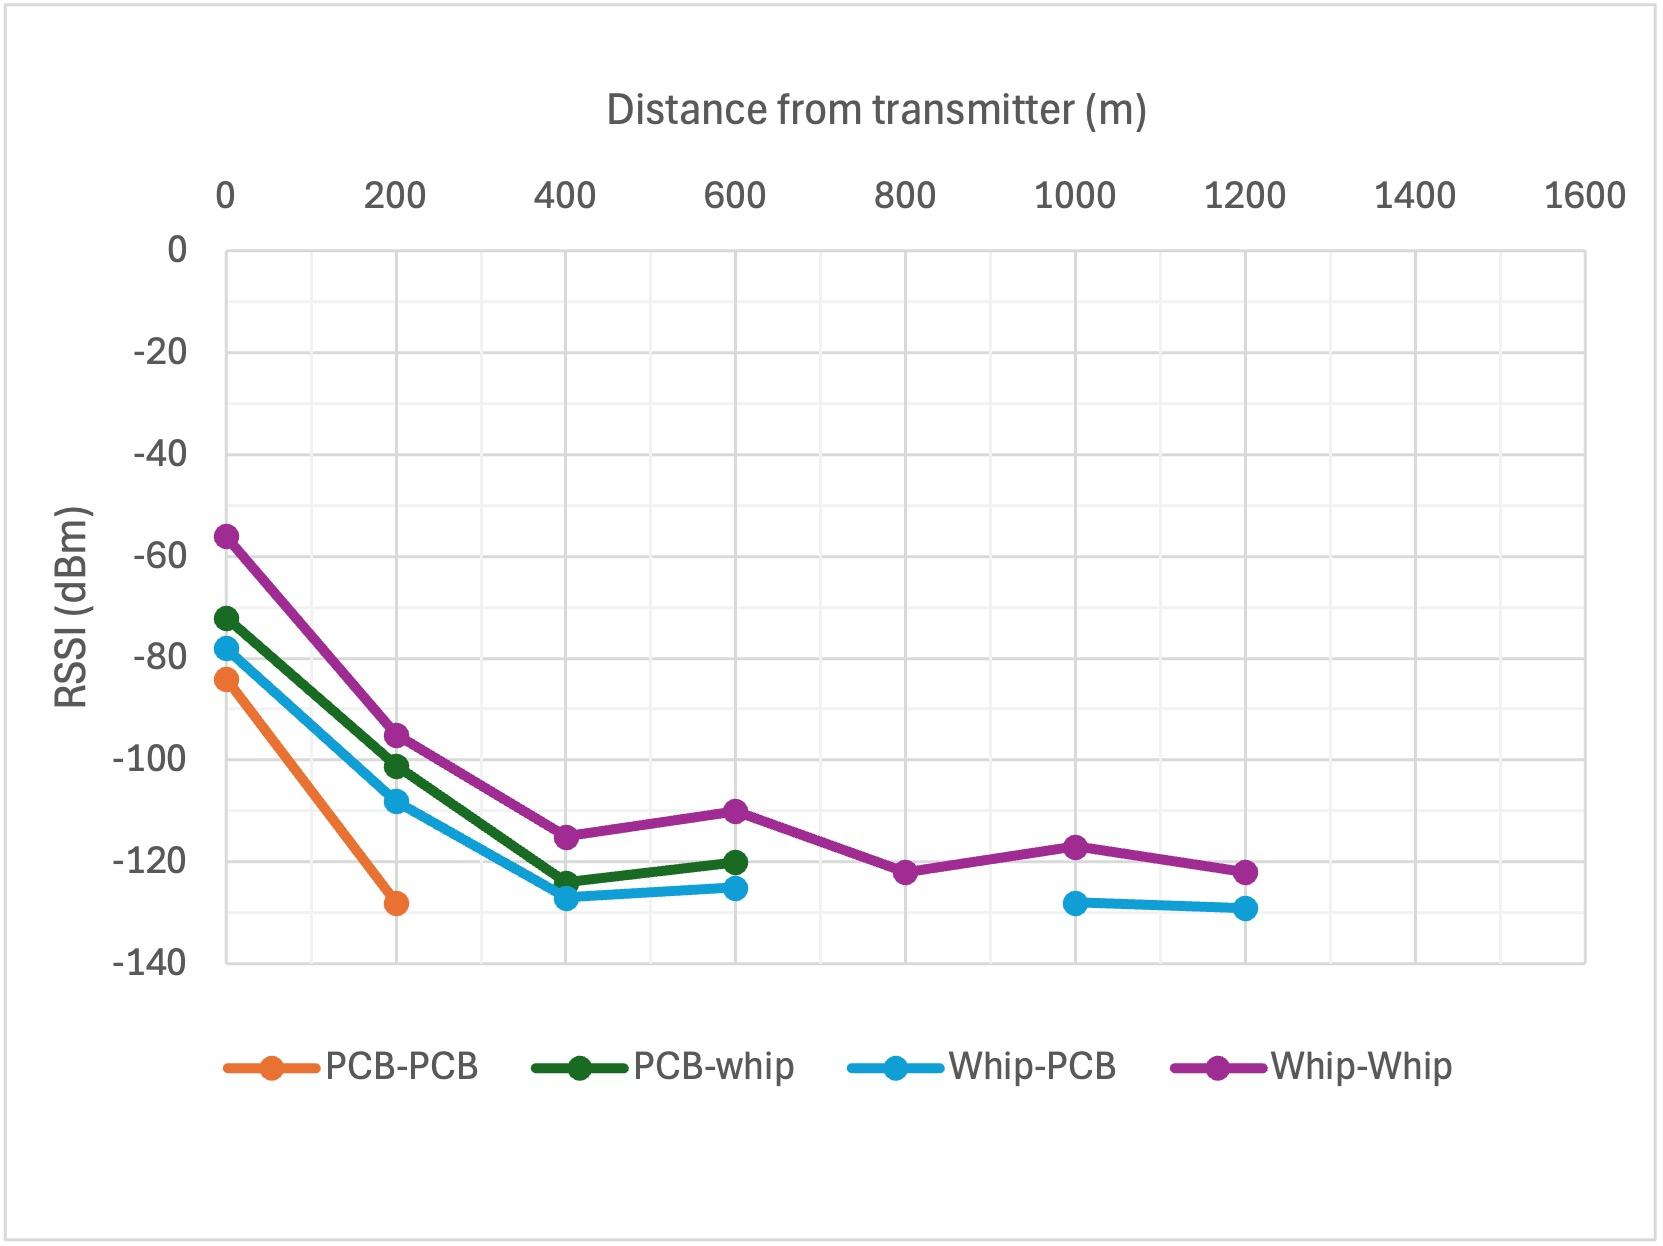
\includegraphics[width=0.9\textwidth]{contents/part-2/fig2/distance-graph.jpg}
    \caption{Graph to show signal loss from different receiver and transmitter configurations (higher is better)}
    \label{fig:range-test-graph}
\end{figure}

Unsurprisingly, the results show that the whip to whip antennas had the best
performance. It was the only configuration that consistently received signal all
the way to 1200m. In contrast with my prediction, the whip to PCB configuration
was the second best and even received a signal at 1200m; although this was less
consistent and had a lower signal strength compared to the whip-whip. I am
unsure why this was superior to the PCB-whip but clearly the increased effective
radiative power had a greater bearing on the RSSI than the sensitivity at the
receiver end. The PCB-whip managed only half the range at 600m and the PCB to
PCB managed just 200m, demonstrating its inadequacy for application in my
project.

\subsection{Battery tests}\label{sec:battery-tests}

There is no mains electricity available in the apple field so the nodes must be
able to operate without an external power source. Even with the use of a solar
panel the node must be able to work through the night and during periods of
dense cloud coverage where the solar panel will not have sufficient power to
keep the node running. This is where the use of a battery is essential as the
solar panel can charge the battery with excess energy during periods of excess
solar radiation, such as during midday hours, and then store this energy for
periods of low or no solar radiation.

However, while daylight will be of little concern during the summer months when
this dissertation is being written, there will be far fewer days of usable
sunlight over the winter period. As the UK has very high latitude, there is
large seasonal variation in the length of a day. For the town of Crediton (the
nearest town to \farmName), in the summer there are 16.5 hours of daylight while
in winter it receives only 7.6 hours; making one night 16.4 hours long.
Therefore the node must have a battery sufficiently large to power it for a
minimum of 16.4 hours with some additional charge to account for high cloud
cover during the early evening and morning period.

To see if the battery solution was sufficient for this environment a test was
run on a fully charged 18650 battery that was then connected to the solar power
manager to allow the voltage to be regulated up to the Challenger's 5V input
voltage.

A digital multimeter was installed between the solar power manager and the
Challenger's usb c input to view the voltage and current in real time as well as
running a timer for the test and a calculation of the number of watt-hours
consumed by the node. The node was then run with a full suite of sensors
attached. During the test the node used 80ma at 5V for a wattage of 0.4W.

The node ran until the battery would no longer discharge, with the final battery
life of the node being 19 hours and 17 minutes. The meter showed that the node
consumed 7.96Wh of power. Considering the battery capacity is 9 Wh it may seem
that the battery ran out too quickly. However, the solar power manager
documentation tells us that the battery boost efficiency - being the conversion
of battery voltage from native 3.7V to 5V output - is only 86\%. With that in
mind the predicted effective capacity is 7.74Wh, which is very similar to the
actual result.

The achieved result of 19 hours should be sufficient for running the node
continuously for much of the year as this compares to the longest night period
of 16.4 hours. However, during periods of heavy cloud cover in winter there is a
chance the node would not be able to charge the battery sufficiently in the day
to allow the node to run over night.

\subsection{Solar panel testing}\label{sec:solar-tests}

The solar panel is rated for 6W maximum power. This however would only
realistically be achieved under optimal conditions with a clear sky and full sun
around midday. This power rating was verified using a multimeter on such a day
where a voltage of 7.02V and an amperage of 0.87A was measured, giving a final
power of 6.1W.

As explained in the battery section above, the node consumed about 7.96Wh over a
19 hour and 17 minute period. We can therefore determine that the node requires
roughly 10Wh of energy per day to able to run continuously. It would be tempting
to then say that the node would need less than 2 hours of ideal sunlight to
operate for an entire day (being 6W * 2h = 12Wh). However we must also account
for the energy loss when converting from raw solar output to the regulated 5V
input that Challenger accepts.

The solar panel manager rates its conversion efficiency for solar at 78\%
meaning for each watt of solar energy received 22\% of this will be wasted as
heat when converted to the correct voltage. If we adjust for this loss we would
need effectively 12.8Wh of energy just to power the node for a day, which
equates to 2 hours and 8 minutes of ideal conditions.

An additional 9Wh is needed to charge the battery which if we adjust again for
solar efficiency factor we get 11.5Wh. This is an additional 1h:55m of ideal
sun, leaving a total sunlight requirement each day of 4h:03m.

\subsection{Hardware assembly and weatherproofing}

Since most of the hardware in this project contains exposed electronics, the
final assembled devices needed to be made wind and water resistant to prevent
failure. However the sensors and solar panel also needed to be exposed to
perform their function effectively - e.g. a solar panel must have a clear view
of the sun throughout the day. The final design therefore needed to balance
multiple conflicting purposes:

\begin{itemize}
    \item The core electronics (Challenger, solar manager, battery etc) must be
          kept dry, cool and away from wind which may damage electronics.
    \item The wind sensor must be exposed to the elements and securely fastened
          to withstand intense wind, it must also be kept high off the ground
          for more accurate readings.
    \item The solar panel must be exposed to the elements and be south facing at
          at an angle of 30-40 degrees to optimise solar efficiency.
    \item The soil moisture sensor must be inserted into the ground and as it
          has exposed electronics must be made waterproof.
    \item The antenna of the Challenger must be placed as high as possible (at
          least 1.5m from the ground).
    \item The temperature/humidity sensor must be exposed to the elements to
          ensure accurate readings but cannot be exposed to rain due to the
          exposed electronics on it.
\end{itemize}

Due to the conflicting nature of some of these requirements, the final device
would need to allow for positioning of different components at different
heights.

The final design therefore was to place most of the sensitive electronics inside
a waterproof box with cut-outs for wiring for external components. This was then
mounted onto a 2m pole to allow for a good antenna signal and more accurate wind
speed readings.

\subsubsection{Sensitive electronics}

An IP65 waterproof junction box (Figure \ref{fig:box-internals}) was selected to
house the non-sensor portion of the electronics. An IP rating measures the
Ingress Protection of a devices housing against water and dust defined by the
International Electrotechnical Commission. The first number of an IP code is a
measure of dust resistance while the second number is a measure of water
resistance. An IP code of 65 therefore means the box used here has perfect dust
resistance and can withstand water jets being sprayed at it from multiple
directions \cite{wiki-ip}. This level of protection should be more than adequate
to withstand the heavy rainfall it will experience.

\begin{figure}[H]
    \centering
    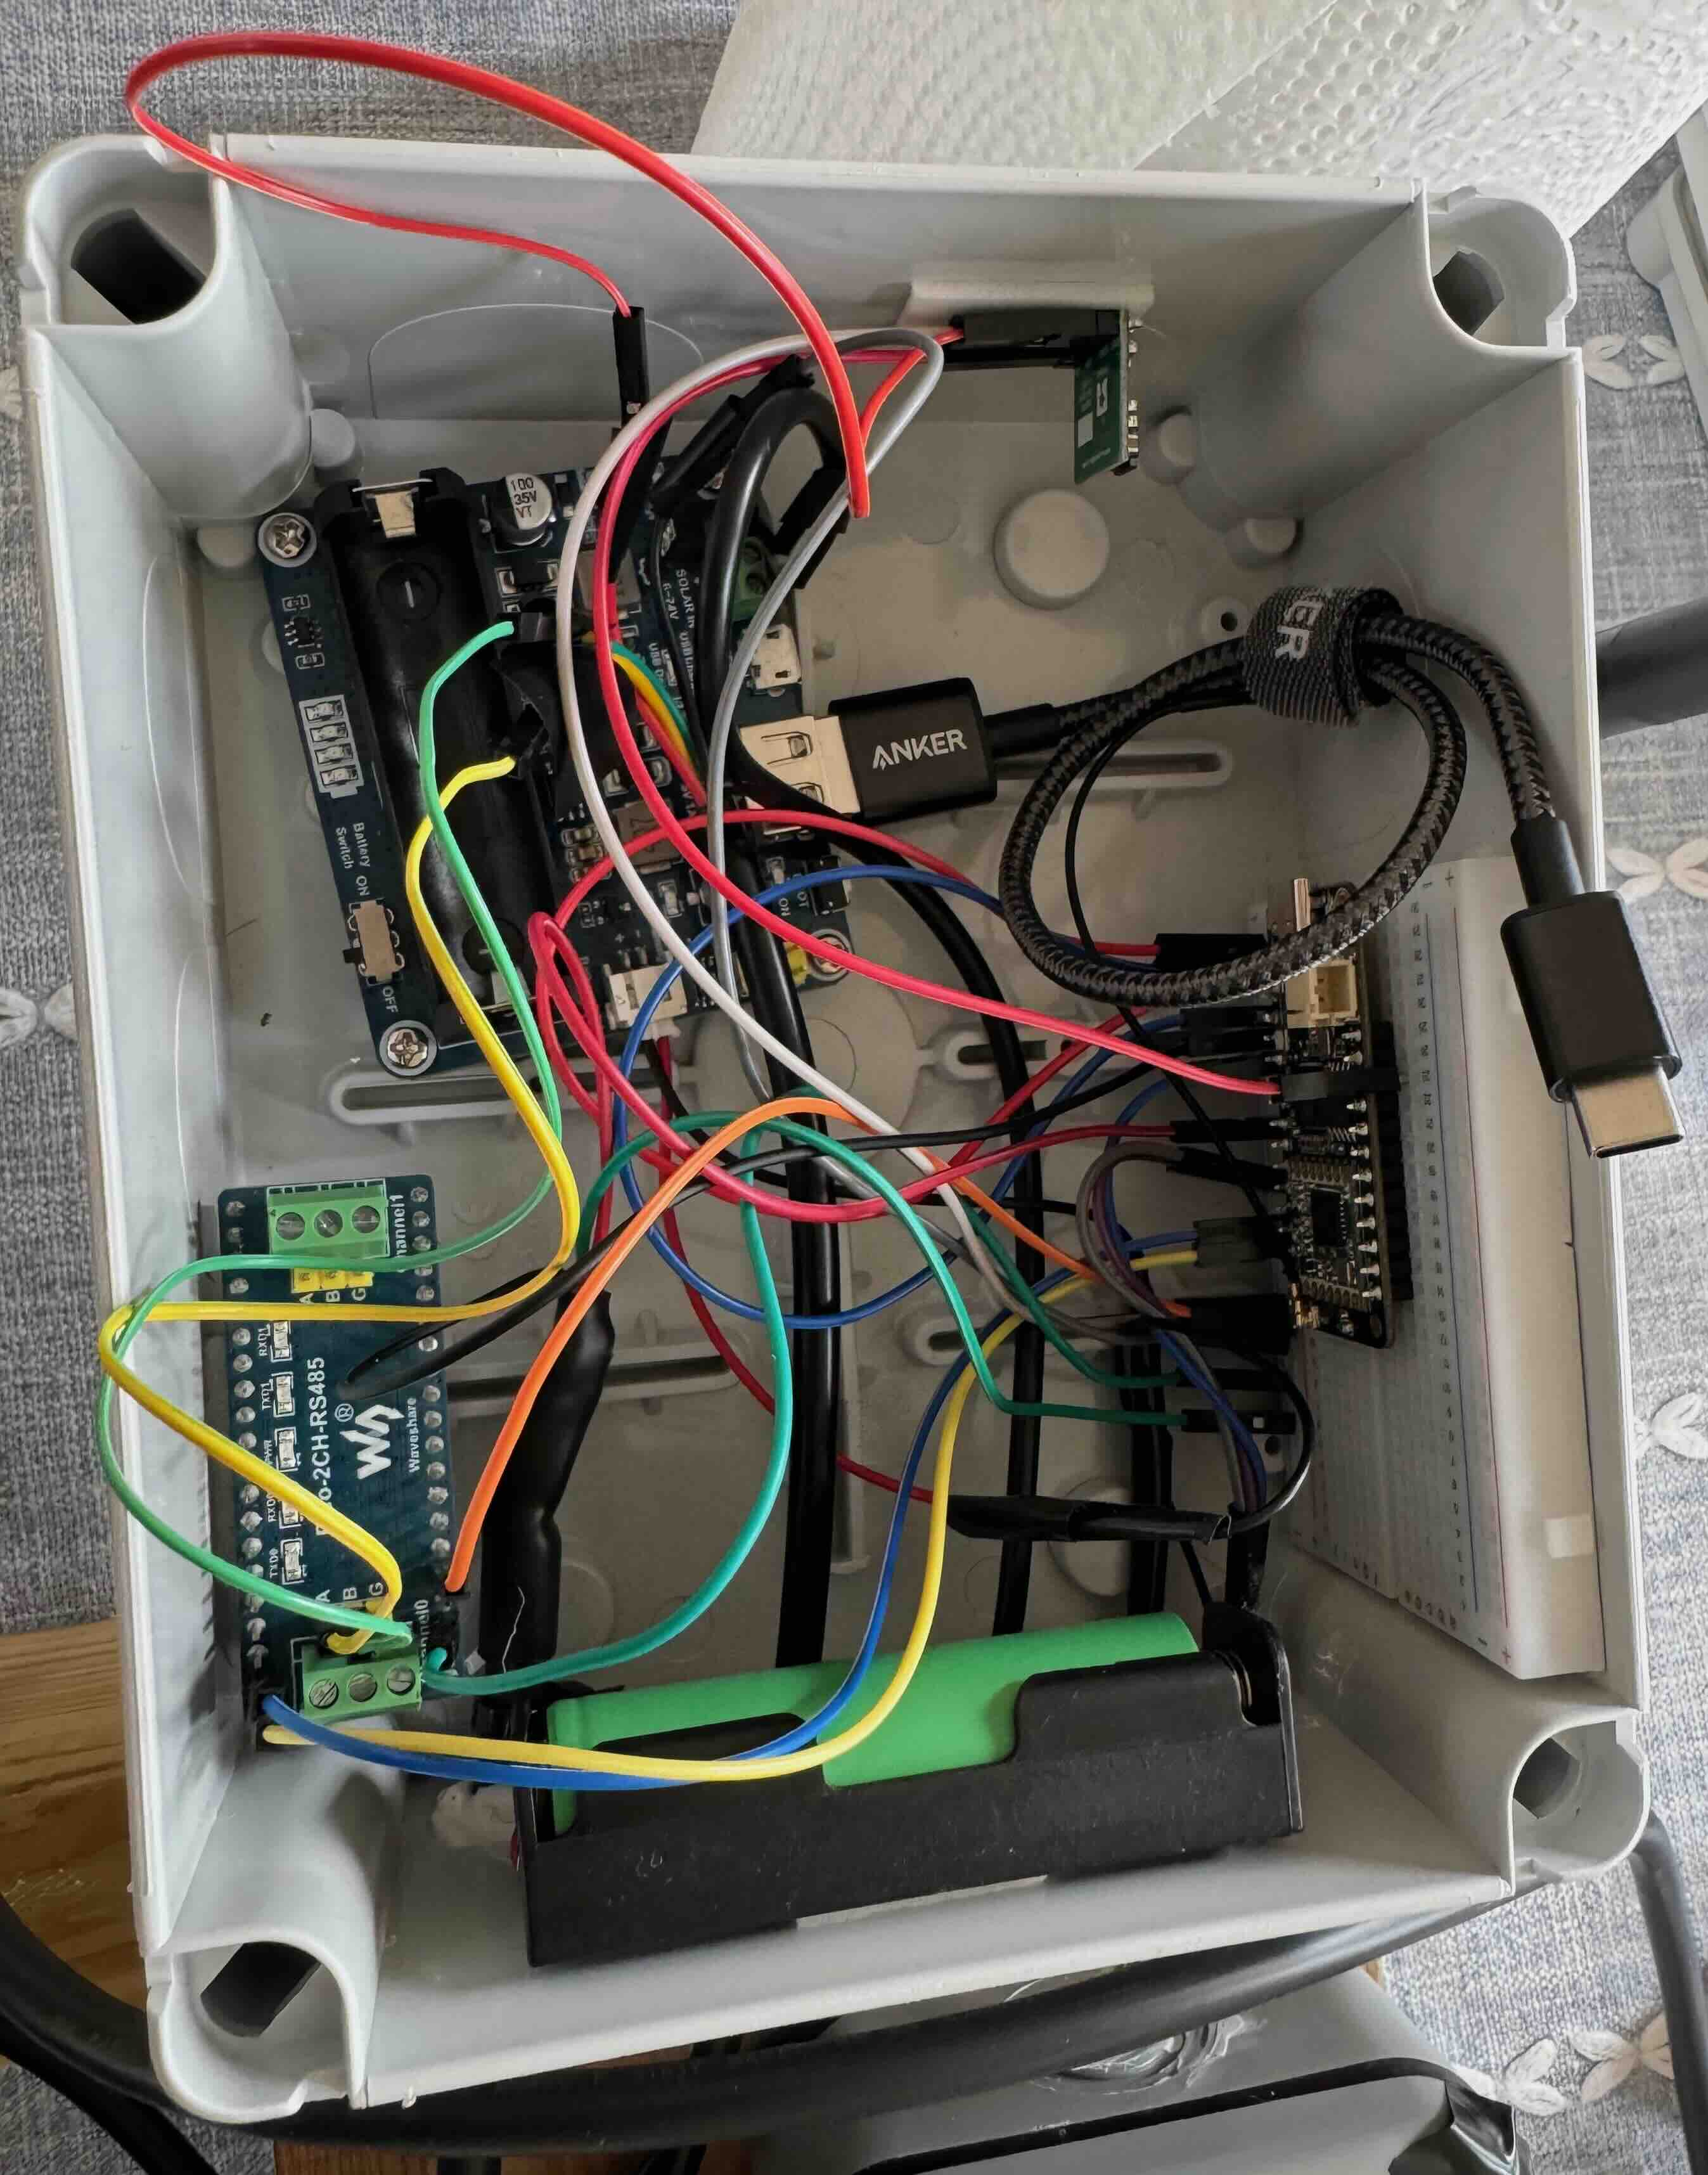
\includegraphics[width=0.5\textwidth]{contents/part-2/fig2/box-internals.jpeg}
    \caption{Open junction box showing internal wiring}
    \label{fig:box-internals}
\end{figure}

The Challenger microcontroller was inserted onto a half size breadboard and then
stuck to one side of the box. The antenna cable was routed to the top right
corner where a small hole was drilled to allow for the antenna to be mounted
externally. All the other components were then wired into the breadboard and
stuck down with double sided sticky pads to prevent damage during transport or
heavy winds. The bottom of the box had holes drilled for the anemometer, soil
moisture sensor, solar panel and temperature/humidity sensor respectively. To
prevent water ingress into these holes, sealant was deposited over the holes.

The entire box was attached to a plank of wood measuring roughly 25cm by 60cm.
This board holds all the sensors with the exception of the soil moisture sensor
which must be able to hang freely.

\subsubsection{Soil moisture sensor}

The sensor that required the most thought as to waterproofing and mounting was
the capacitative moisture sensor. The first challenge was the need for the soil
moisture sensor to be able to reach ground level while the microcontroller
collecting its readings was secured 2m above it. The solution to this was to
swap the small included wires with a 2.5m weatherproof cable containing three
cores (one for power, one for ground and one for data). Each cable core was then
soldered onto the sensor as in figure ~\ref{fig:solder-soil}, allowing for the
sensor to be inserted into the ground.

\begin{figure}[H]
    \centering
    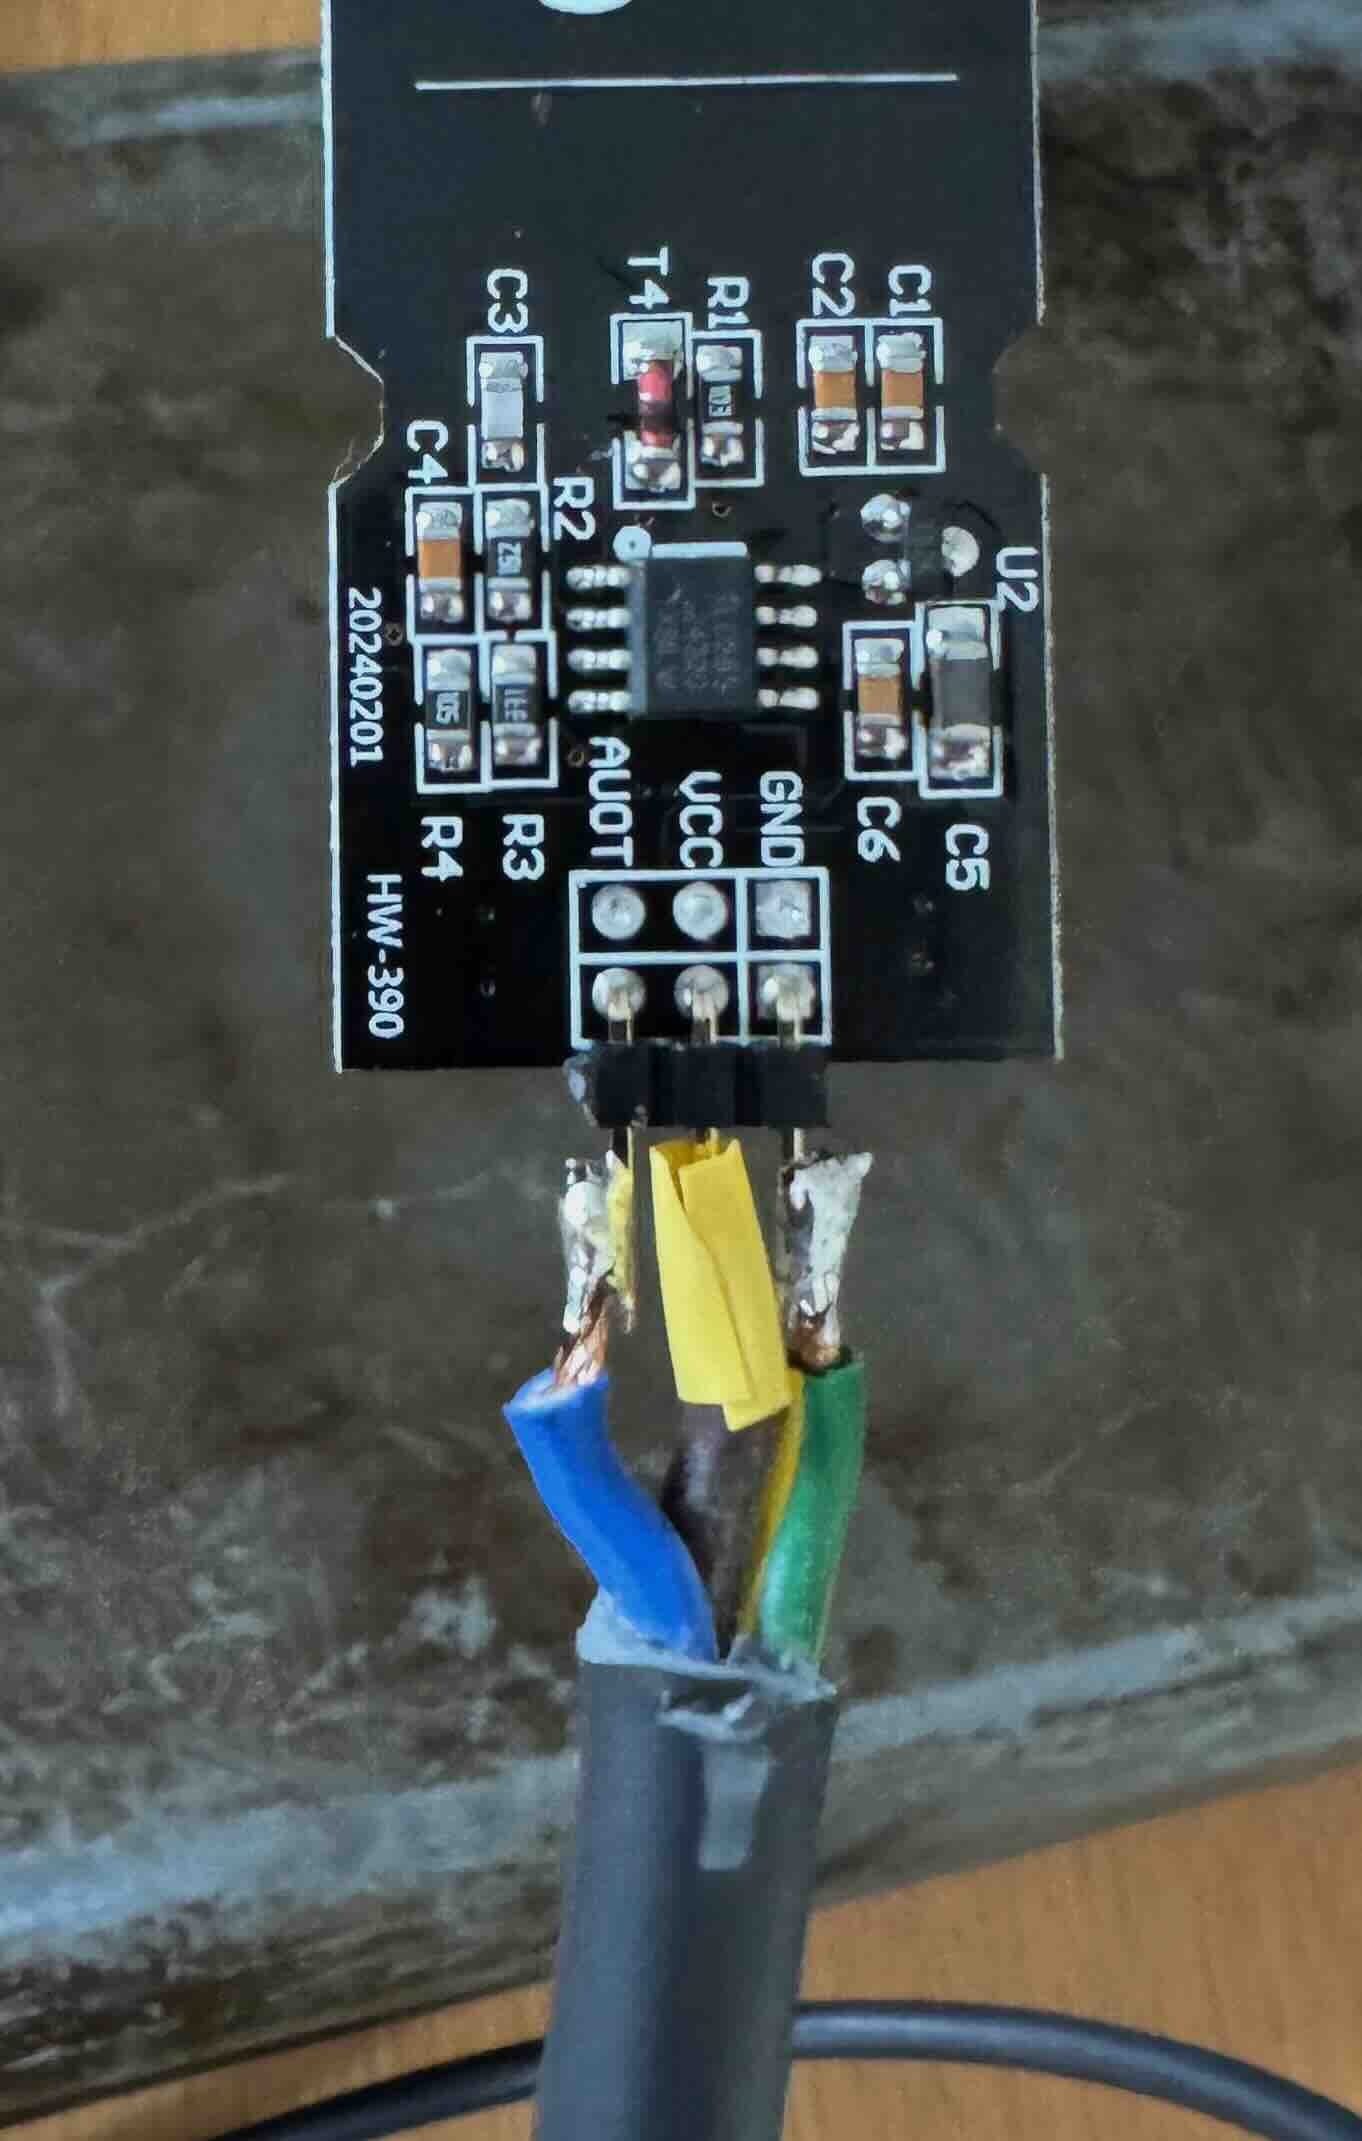
\includegraphics[width=0.25\textwidth]{contents/part-2/fig2/solder-soil.jpeg}
    \caption{Soldered soil moisture sensor}
    \label{fig:solder-soil}
\end{figure}

Waterproofing the sensor was necessary as while the bottom three quarters of the
board are designed to be inserted into soil, the part above this is made up of
exposed electronics that must not come into contact with water (Refer to figure
~\ref{fig:soil-sensor}). This means it was essential to waterproof this part of
the board.

To achieve this I followed an online tutorial on a hobbyist website
\cite{waterproof-sensor}. and painted the electronics using nail varnish. While
this sounds unconventional, nail varnish is a non-conductive compound that can
be easily painted over electronics using the brush included and so is quite a
popular low-cost method for waterproofing electronics. After this is applied the
portion of the board with the electronics is covered in heatshrink to form a
tight seal over the board, with a layer of nail polish on the edges to reduces
the chance of water ingress under the heat shrink's plastic.

\subsubsection{Other external components}

The DHT11 sensor was mounted inside a smaller IP55-rated junction box, which
provides the same resistance against rain as the larger box. To allow for more
accurate readings, small holes were drilled on the bottom panel of this so the
air temperature inside the box would better match the external
temperature/humidity. To further improve the sensor's accuracy, the box was
painted white to reflect sunlight, and a solar shield made from a cut and
reshaped aluminium can was mounted to the south facing side. This shield (see
red box in Figure \ref{fig:solder-soil}) helps to prevent the sensor being
exposed to direct sunlight, reducing temperature distortion while still allowing
airflow from the sides.

The solar panel was mounted below the main enclosure using the included
adjustable gimbal mount. It was fixed at an angle of approximately 40° from
horizontal, which balances solar efficiency throughout the year
\cite{cathcart_best-solar-panel_2025}. This angle is steeper than the optimal
summer setting but allows for improved performance during winter months when the
sun is lower in the sky. The gimble allows for rotation in all planes which is
useful in case the box itself cannot be mounted in a perfect southerly
direction.

The anemometer was secured to a separate length of wood, positioned
approximately 0.5 metres away from the main unit. This separation reduces
turbulence caused by the box and pole, leading to more accurate wind speed
readings. The sensor was screwed directly into the wood and positioned at a
height of 2m.


\begin{figure}[H]
    \centering
    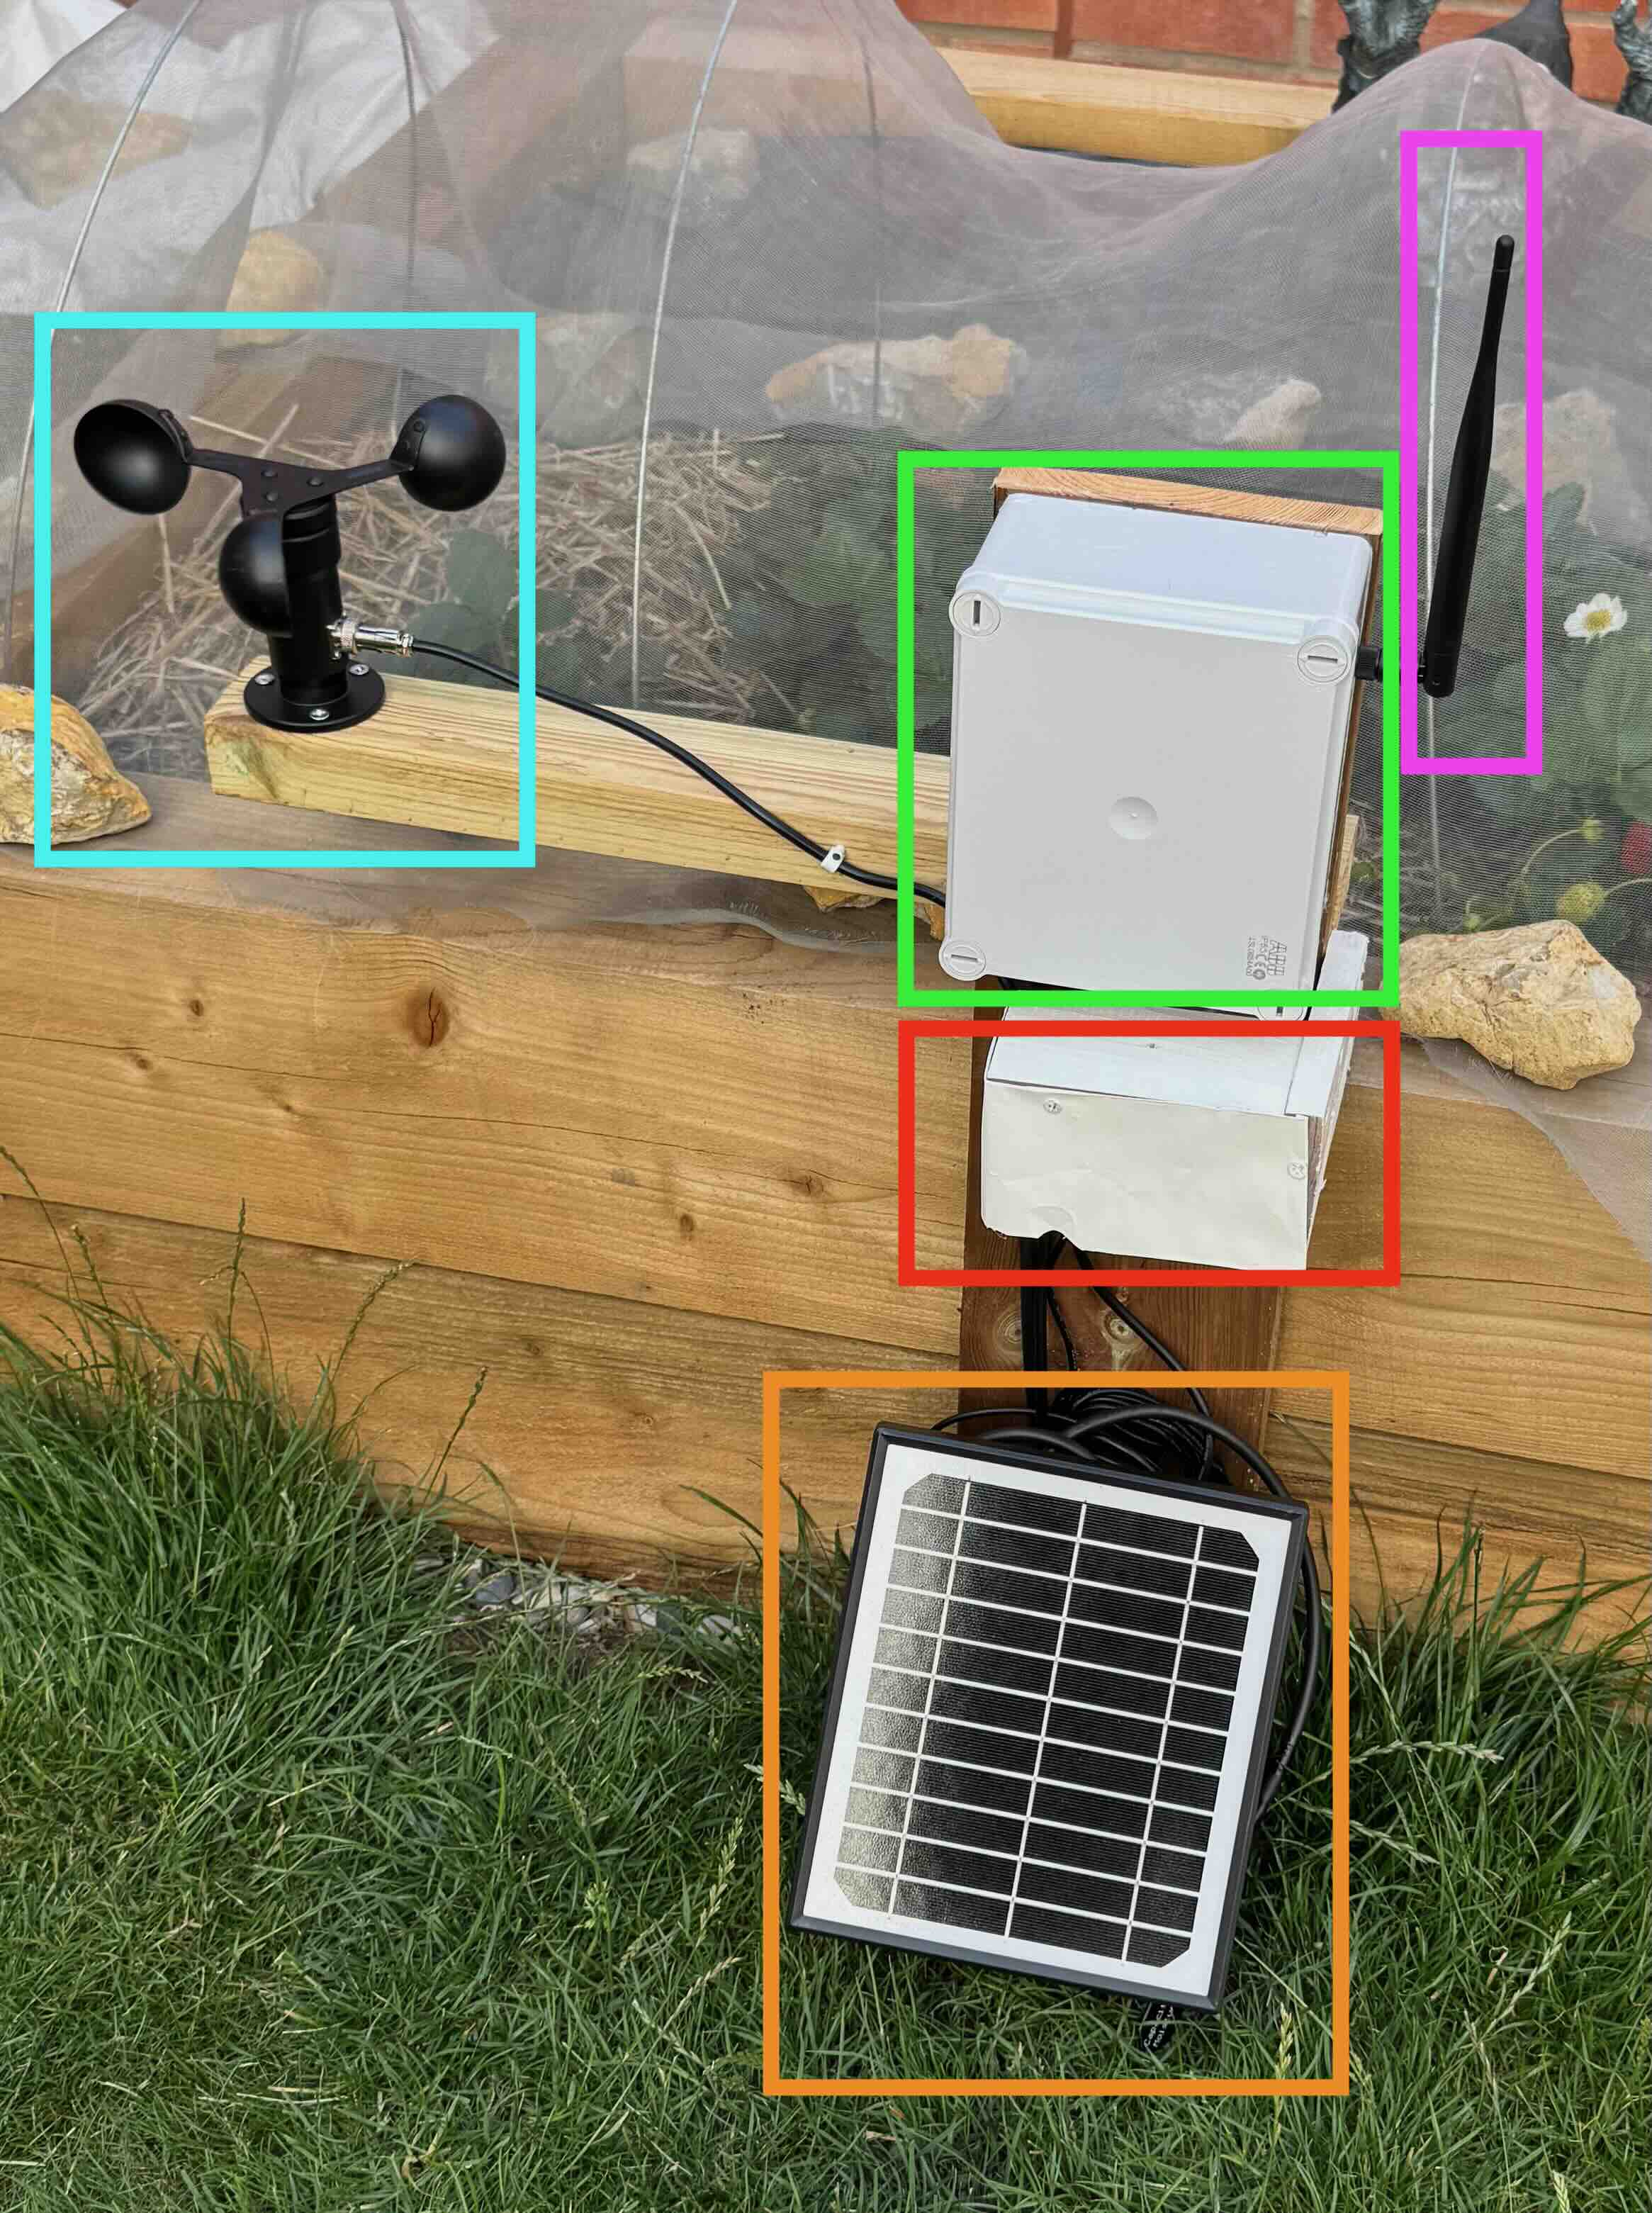
\includegraphics[width=0.6\textwidth]{contents/part-2/fig2/annotated-node.jpg}
    \caption{Final node design}
    \label{fig:assembled-node}
\end{figure}

Figure \ref{fig:assembled-node} shows the final assembled node. From top to
bottom, the purple box shows the antenna, the blue box shows the anemometer on
its separate arm, the green box contains the electronics, the red box is the
solar shield that surrounds the temperature/humidity sensor and the orange box
shows the solar panel. Not pictured is the 2m wooden post that extends the
height of the node.

\subsubsection{Gateway}

\begin{figure}[H]
    \centering
    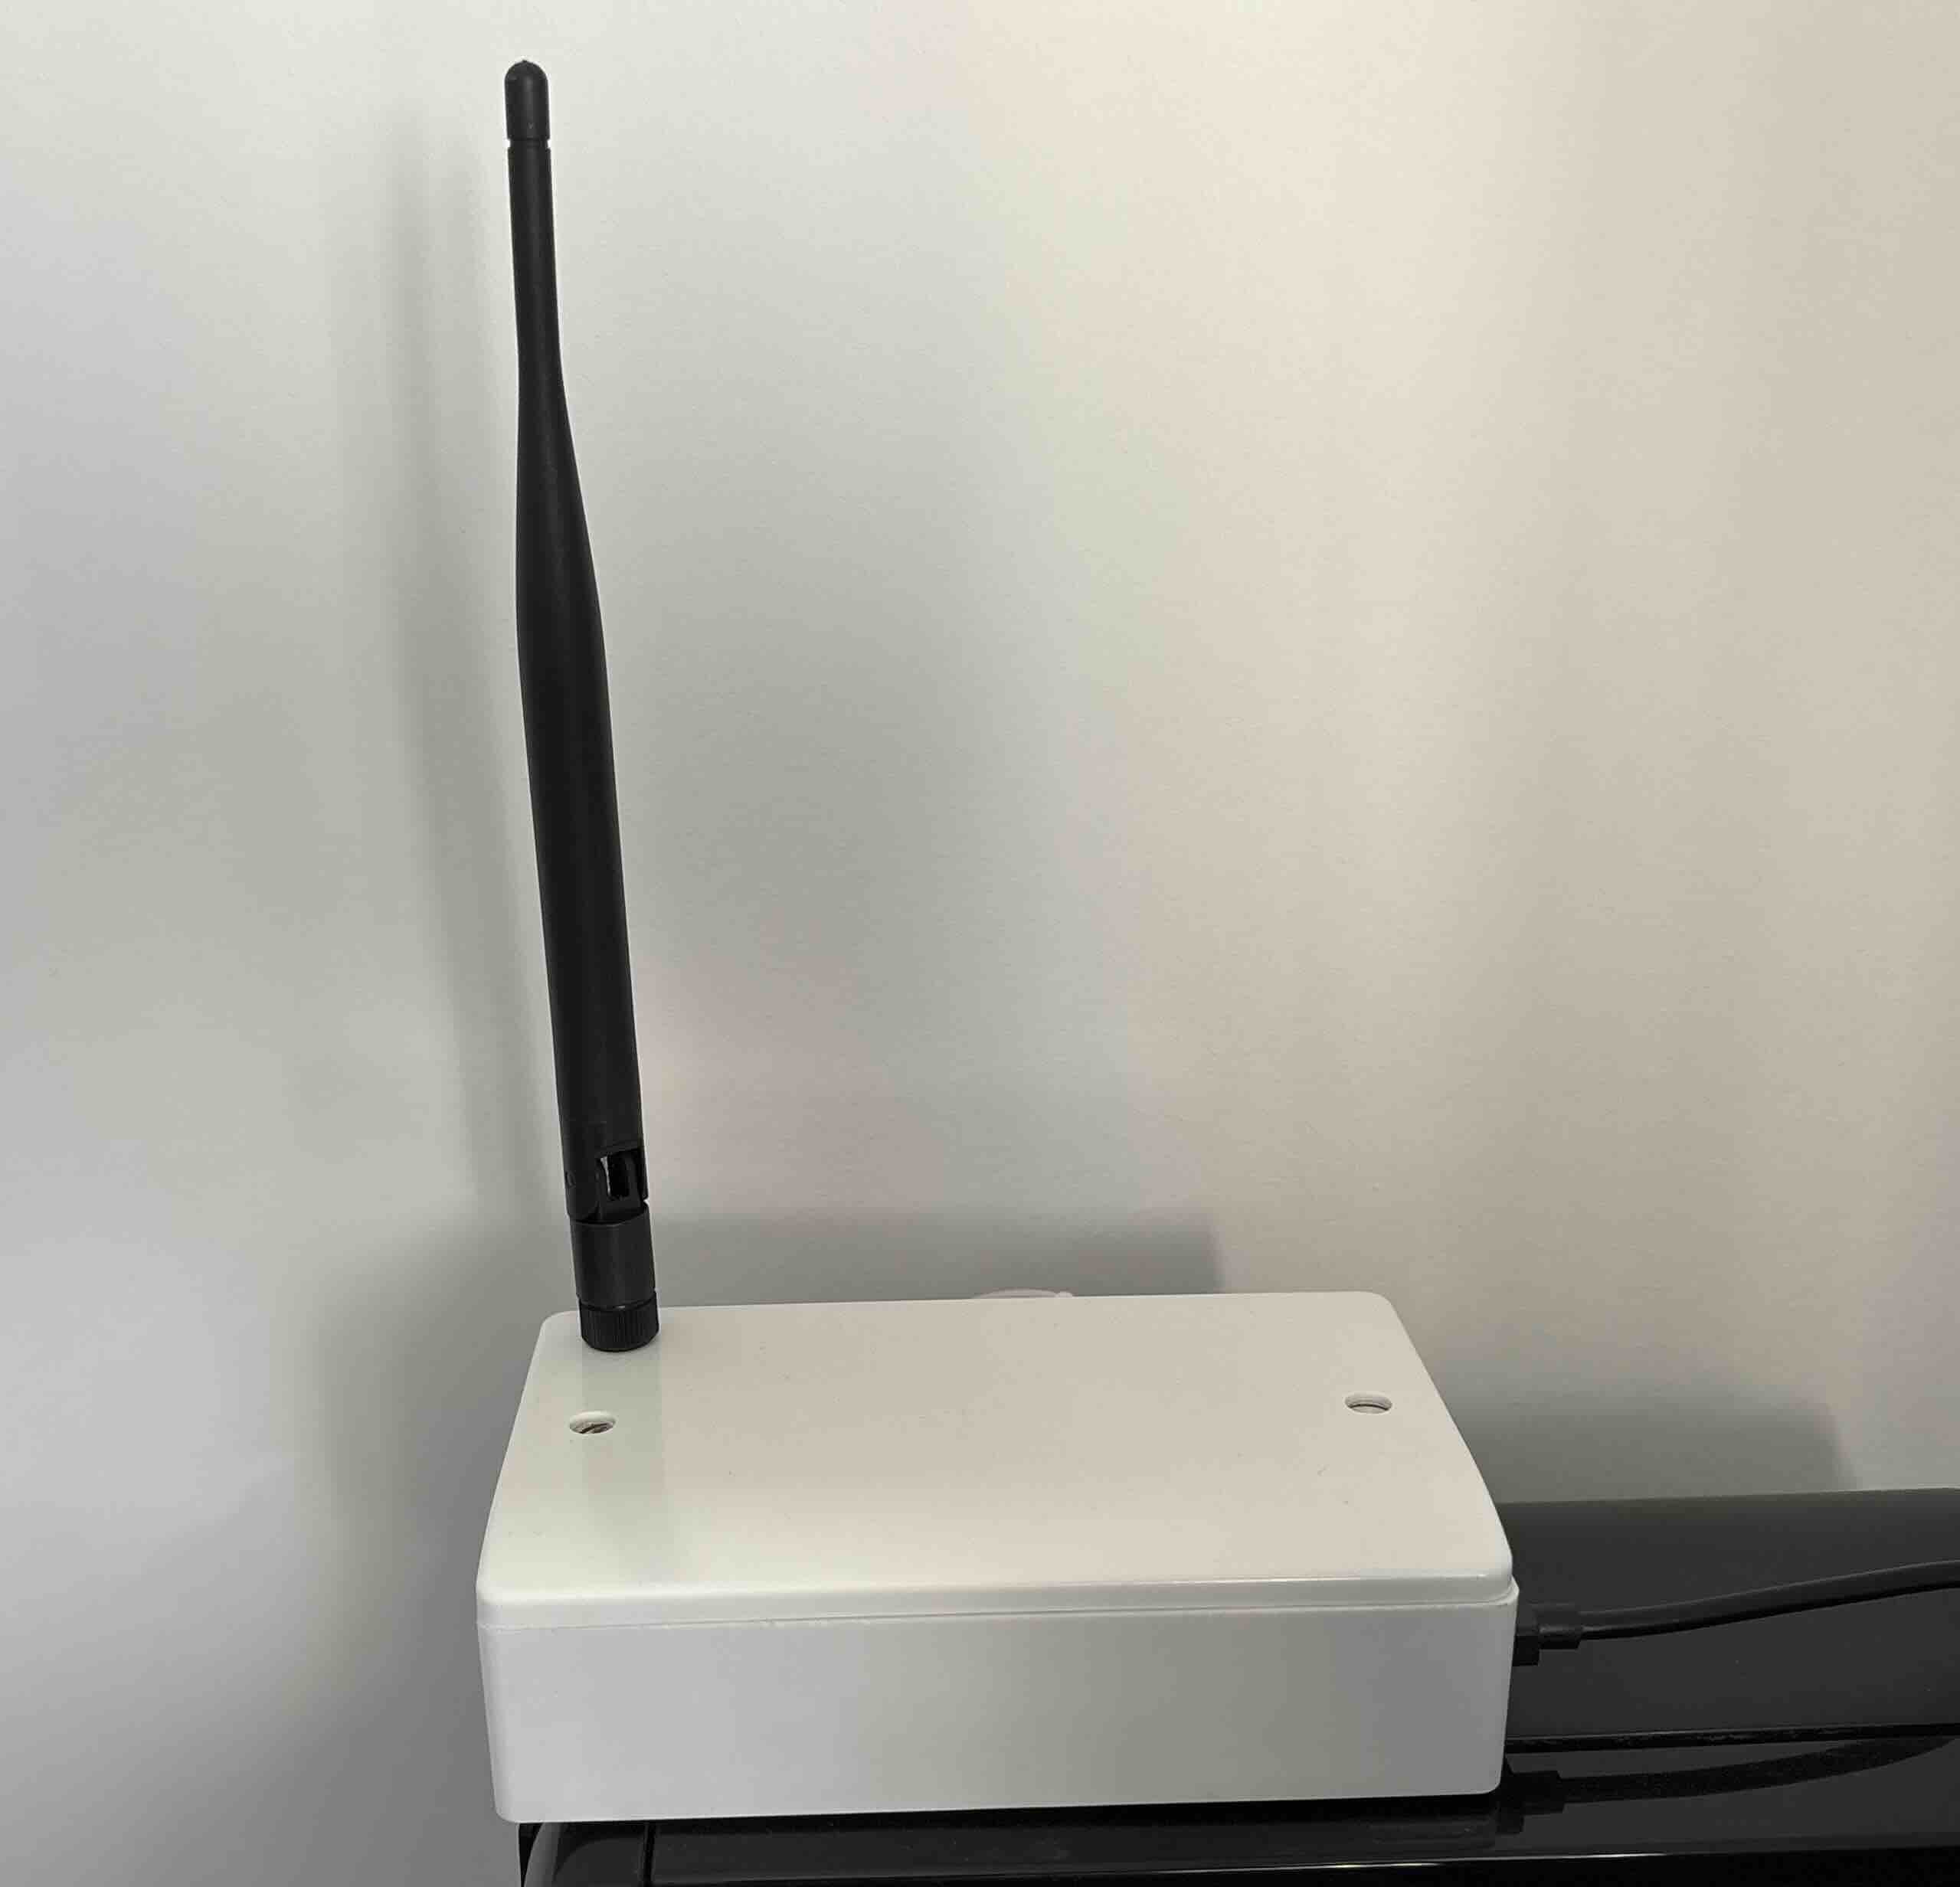
\includegraphics[width=0.4\textwidth]{contents/part-2/fig2/gateway.jpeg}
    \caption{Completed gateway}
    \label{fig:gateway-final}
\end{figure}

The gateway node (Figure \ref{fig:gateway-final}) required less careful
engineering as there was no requirement for it to be waterproofed or mounted
externally. As this would eventually be placed inside a private home, the aim
was to make it minimally imposing so a design similar to an internet router was
chosen.

The two devices inside the box were the Raspberry Pi and the Challenger. A
plastic box was used with cut outs for the Pi's outputs and power cable, with an
additional cut out on the lid for the Challenger's antenna. The Pi and
Challenger were then secured to the box's base with velcro tape, as both devices
would potentially need to be removed for trouble shooting.

\section{Deployment}

\subsection{Test deployment at home}

Before setting up the nodes at the farm it was important to run the equipment in
an area where repairs and updates could be more easily performed. The nodes were
therefore placed at different locations in my garden and ran continuously from
the 15th of August.

\subsubsection{Challenges and solutions from test deployment}

One of the first challenges from the test deployment was the fact the batteries
on the nodes were not quite sufficient to allow 24/7 readings. On the fourth day
of the run, after an overcast evening the night before, one of the nodes stopped
transmitting at around 6am - just before sunrise. To remedy this another battery
was fitted to each of the end nodes (but not the repeater as this had much lower
battery consumption from the lack of any sensors). This doubling of battery
capacity would make loss of power during the night much less likely. The fact
the solar panels could charge the battery fully by mid morning pointed to the
fact that solar capacity was sufficient but battery capacity was not.

A related problem was that when the node died it did not start repeating again
after this despite solar power returning and the battery getting recharged. I
discovered that when the microcontroller detected brownout - being a sudden dip
in voltage - the device would enter a safeboot mode. In this safeboot mode the
default code.py file would not automatically be run and instead the device would
create and use a safemode.py file that without modification would essentially
run infinitely unless the reset button on the device was pressed or the device
was powered off and on again.

Clearly this behaviour was not appropriate for field deployment where brownouts
would potentially occur whenever the battery was discharged completely. Even
with the additional battery capacity provided by a second battery there would
still be a high chance of this occurring on particularly dark days during
winter, where continuous uptime could not be guaranteed.

To remedy this, I modified the safemode.py file using a template I found in the
circuitpython documentation. This version of the safemode.py file was made
specifically for the case I was using i.e. remote solar powered projects where
manual reset of the board could not be achieved easily. Instead of entering an
infinite loop this safemode would (DESCRIPTION OF SAFEMODE).

A seperate issue was the behaviour of the temperature-humidity sensor when
exposed to direct sunlight. While the junction box used to encase the sensor was
painted white to reduce any heat transfer from solar radiation, the readings
taken on very sunny days showed a large delta of around 5 celsius between the
sensor readings and local air temperature readings that could not be explained
with the existence of a microclimate.

To reduce this effect an additional solar shield was made to surround the
sensor. Consisting a wooden frame and aluminium shield to block light falling on
the junction box. While this method did help to reduce the delta at midday to
around 3 celsius there was still clearly quite a pronounced effect. So to
further reduce any warming the solar panel was mounted to the rear of the node.
This would allow the temperature sensor to face north instead of south which in
the northern hemisphere would result in much reduced solar warming to the
sensors box as the sun tracks over the southern area of the sky in the UK.

\subsection{Deployment in the field}

\subsection{Placement of nodes}

\part{Software development}

\section{Programming the hardware}

Section on programming: 1) The nodes, 2) the repeater, 3) The gateway

The challenger boards can be programmed in a few different languages. The most
common of these are C (including C++) and python. I decided to program the
boards in python due to the large availability of sensor libraries written in
this language. Programming in C, while potentially more efficient, would likely
have meant I would need to write my own libraries and functions to get many of
the sensors to function properly and therefore was not selected.

The RP2040 processor of the challenger uses relatively low power, so the
versions of python for the chip tend to be stripped down to accommodate this.
The two main python versions available are circuit python and micropython. They
both have extensive libraries and work with all the sensors I have selected.
With no major difference in their functionality, I settled on circuitpython as
this was the version recommended by iLabs (the makers of the challenger board)
and included a library that supports challenger as well as example code.

\subsection{LoRa settings configuration}

The most fundamental part of the program for each of the nodes in the LoRa
network was that they could communicate with each other. This required the
careful matching of LoRa configuration settings between them.

    {ADD LoRa settings}

LoRa has many parameters that must be aligned for two devices to communicate
successfully. These include:

\begin{enumerate}
  \item \textbf{Spreading factor:} 
  \item \textbf{Frequency:} Must match across devices; this project uses
  868\,MHz, the UK LoRa ISM band.
  \item \textbf{Bandwidth:} Determines how wide the signal is, I am using
  125\,kHz.
  \item \textbf{Coding rate:} 
  \item \textbf{Transmit power:} Affects the power and therefore range. This
  must be set within legal limits (e.g., 14\,dBm in the UK).
\end{enumerate}

\subsubsection{Compliance with regulatory limits on radio power}

The UK has strict regulations on the usage of radio transmitters under the Ofcom
ISM band rules. For the 868mhz band, the maximum effective radiated power that
can be used is 25mW. This corresponds to a transmit power of roughly 14dB.

Additionally, the UK has rules on duty cycle rates. This is essentially how long
radio signals are permitted to be on air. For example at a spreading factor of
12 a message may take approximately 1 second to send. The duty cycle limit in
the UK is 1\%, meaning you may only transmit for 1\% of the time on a given day.
1\% of a day is 864 seconds. This means to stay in line with UK regulations only
864 messages could be sent on a given day - or roughly 1 message every 2
minutes.


\subsection{Sensor nodes}

\subsection{Repeater}

\subsection{Gateway}

\subsection{Remote diagnostics and error handling}

Since all the sensors would not be accessible easily errors needed to be
reported remotely to diagnose faults and problems. Unfortunately, while the
sensor nodes and repeater are technically network connected with LoRa there is
no easy way to send firmware updates over the air without developing a program
to accept and create new files over LoRa (FACT CHECK THAT), which was outside
the scope of a three month dissertation. Therefore instead the nodes would need
to have robust error handling written into their programs.

Diagnostics on the gateway node was luckily much simpler as this was powered on
24/7 and network connected. (EXPLANATION OF TAILWIND AND RVC VIEWER)


\section{Overview of software design}

\section{Backend: Database and SQL API}

For the database, I chose Render as a good low cost option for hosting the web
service as it offers a free trial period, constant uptime and backups. The free
version of web services by Render (render.com), provides a limited set of
resources at zero cost: 256 MB of RAM; 0.1 share of a CPU and 1 GB of storage.
There are also limits on outbound bandwidth, build pipeline minutes and instance
hours. A single instance of a POSTGRES database is available on this service -
which is free for the first 30 days and then costs \$5 a month. These resources
should be sufficient for this project as only small amounts of data are
involved.

The web service is running an API I have written, which will receive data from
the raspberry pi used as the gateway. The data is sent using a POST request
with a JSON body which is parsed, processed and added to the database by the
API. Data can be retrieved for display by the frontend using a GET request.

The database design is very simple with a single table holding all the data so
the choice of database management system is not crucial. Having said that,
POSTGRES is a well established and reliable relational database management
system that complies with ANSI SQL standards and most importantly for this
project is supported by Render.

The 1 GB storage limitation allows for (x) rows of data with the current
database design.

This solution should scale well. Additional tables can be added to the POSTGRES
data base for additional sites. And in the unlikely event that the volumes
exceed the Render limits it is easy to pay more for additional resources.

\section{Frontend: Agriscanner webapp}

Overview of front-end

\section{Forecasting with machine learning}

\part{Evaluation}

\section{Hardware evaluation}\label{hardware-evaluation}

\subsection{Qualitative discussion of weather station performance}

\subsubsection{Battery life, solar power and
  outages}\label{sec:hardware-evaluation-power}

The nodes have had more downtime than expected based on the energy budgets in
Sections~\ref{sec:battery-tests} and~\ref{sec:solar-tests}, despite doubling the
battery capacity during deployment. The primary cause is site placement, with
both nodes in a north-facing garden bounded by 2.5\,m fencing and a two-storey
house immediately to the south. As a result, they receive no direct sunlight
until 09:00, and Node 1 is shaded again by 15:00 due to the shadow of a nearby
garage. This leaves only \(\approx\)5\,h of direct sunlight, which is far below
the amount assumed in the design of the nodes.

Outages seem to only affect the sensor nodes; the repeater has had zero downtime
since installation. This is consistent with its much lower energy budget from a
lack of any peripheral sensors, which reduces average energy draw.

The limitations of the current location, plausibly explain the observed outages.
Because these shading conditions are unlikely in an open field, these outages
are not of primary concern for the intended deployment. However, it highlights
the system's sensitivity to late sunrise and early sunsets from terrain. This
would potentially be an issue if the actual deploy site was shaded by a hill or
some tall trees late in the day, which I had not properly considered in the
design phase.

\subsubsection{Weatherproofing}

The summer of 2025 is set to be one of the hottest and driest on record with
August specifically receiving roughly half its average rainfall
\cite{uor2025summer}. Consequently, from the 15th of August to the 26th of
August the weather stations saw only short spells of rain, making an analysis of
their weather proofing hard to review up to this point.

Fortunately, from the 27th August onwards the nodes were exposed to fairly heavy
sustained rainfall. Throughout this period there has been no evidence of water
ingress.

Beyond ingress testing, the nodes experienced elevated ambient temperatures
(exceeding \SI{32}{\degreeCelsius}) and showed no signs of overheating. These
results are encouraging, although longer-term deployment that includes colder
weather and sustained heavy rain is needed to comment conclusively on their
overall robustness.

\subsubsection{Range}\label{sec:range-eval}

As reported in section ~\ref{sec:range-tests} the Challenger microcontrollers
and antennas used in this configuration are able to reach at least 1200m of
range in a real world situation. The conditions in that test were not ideal for
LoRa as both the receiver and transmitter were positioned low to the ground at
around 1-1.5m. In addition line of sight was broken at around 1000m which
severely diminishes the performance of any radio communication system. There
were also buildings between 1200m and 1400m that blocked LoRa signals entirely.

In the intended deployment of my full weather network, the use of an additional
repeater would significantly improve range. In a flat terrain setting the use of
a repeater would double the range. If terrain is hilly a repeater can increase
range by even larger multiples. The below graphic demonstrates the problem of
hills when it comes to LoRa. As a LoRa signal propagates from the transmitter
and collides with a hill the majority of the signals energy is reflected off the
hill meaning it cannot reach the gateway.

\begin{figure}[H]
  \centering
  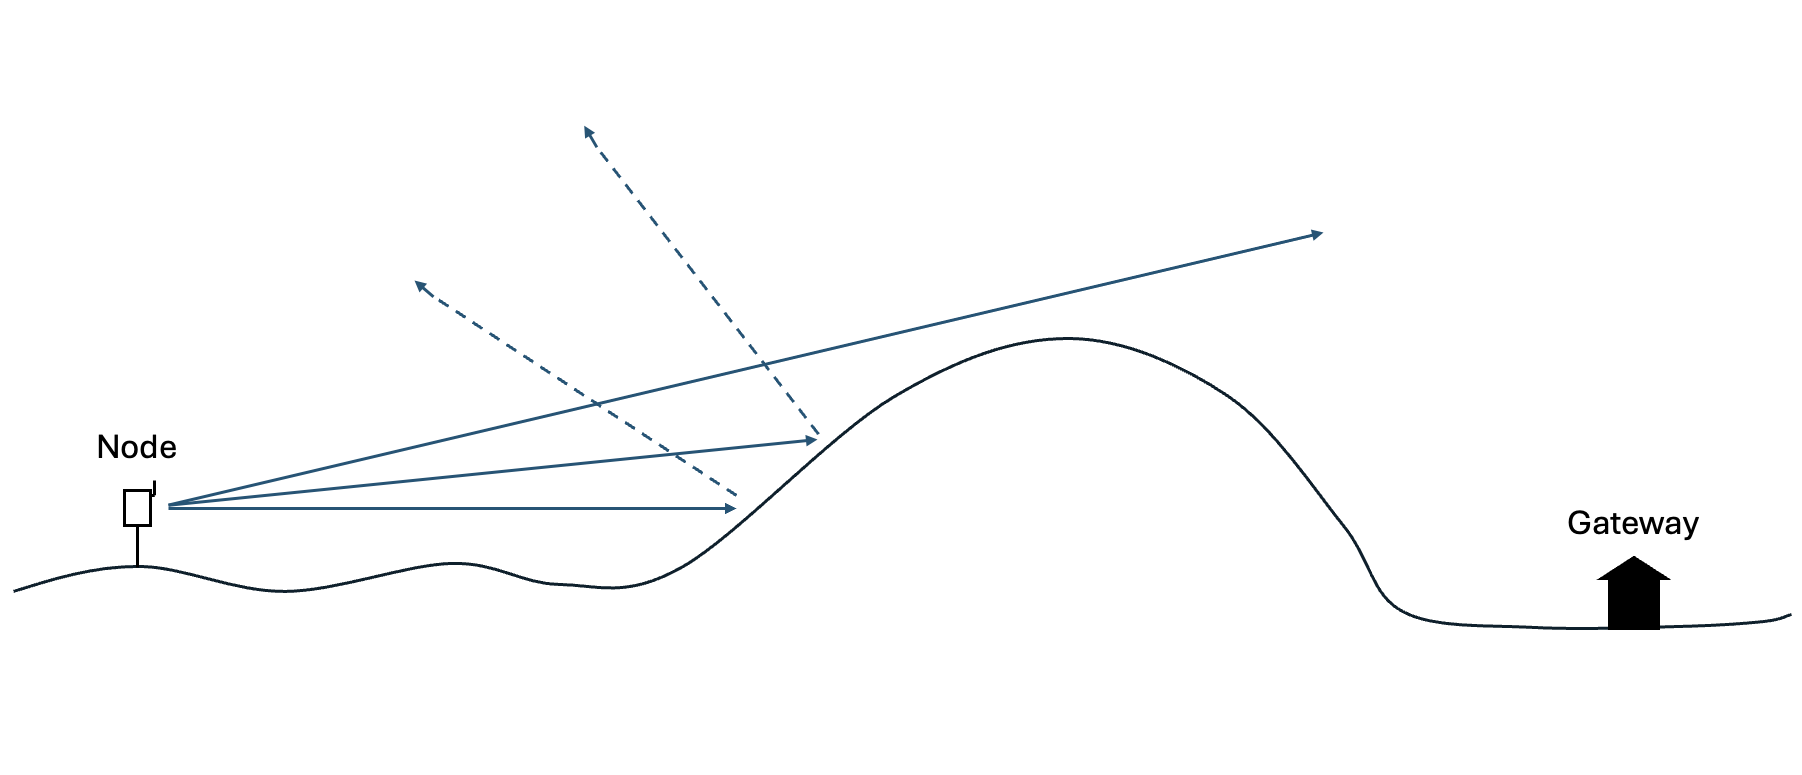
\includegraphics[width=0.9\textwidth]{contents/part-4/fig4/no-repeater.png}
  \caption{Illustration of LoRa radio propagation between node and receiver with blocking terrain}
  \label{fig:no-repeater}
\end{figure}

If a repeater is placed on the top of the hill not only would it mean the LoRa
signal would reach the gateway but the repeaters increased elevation would give
a significant boost to its range as the total area with a line of sight to the
repeater would be vastly increased.

The range that this repeater allows is what sets the design of my network apart
from commercial options and is discussed in more detail in the next section..

\begin{figure}[H]
  \centering
  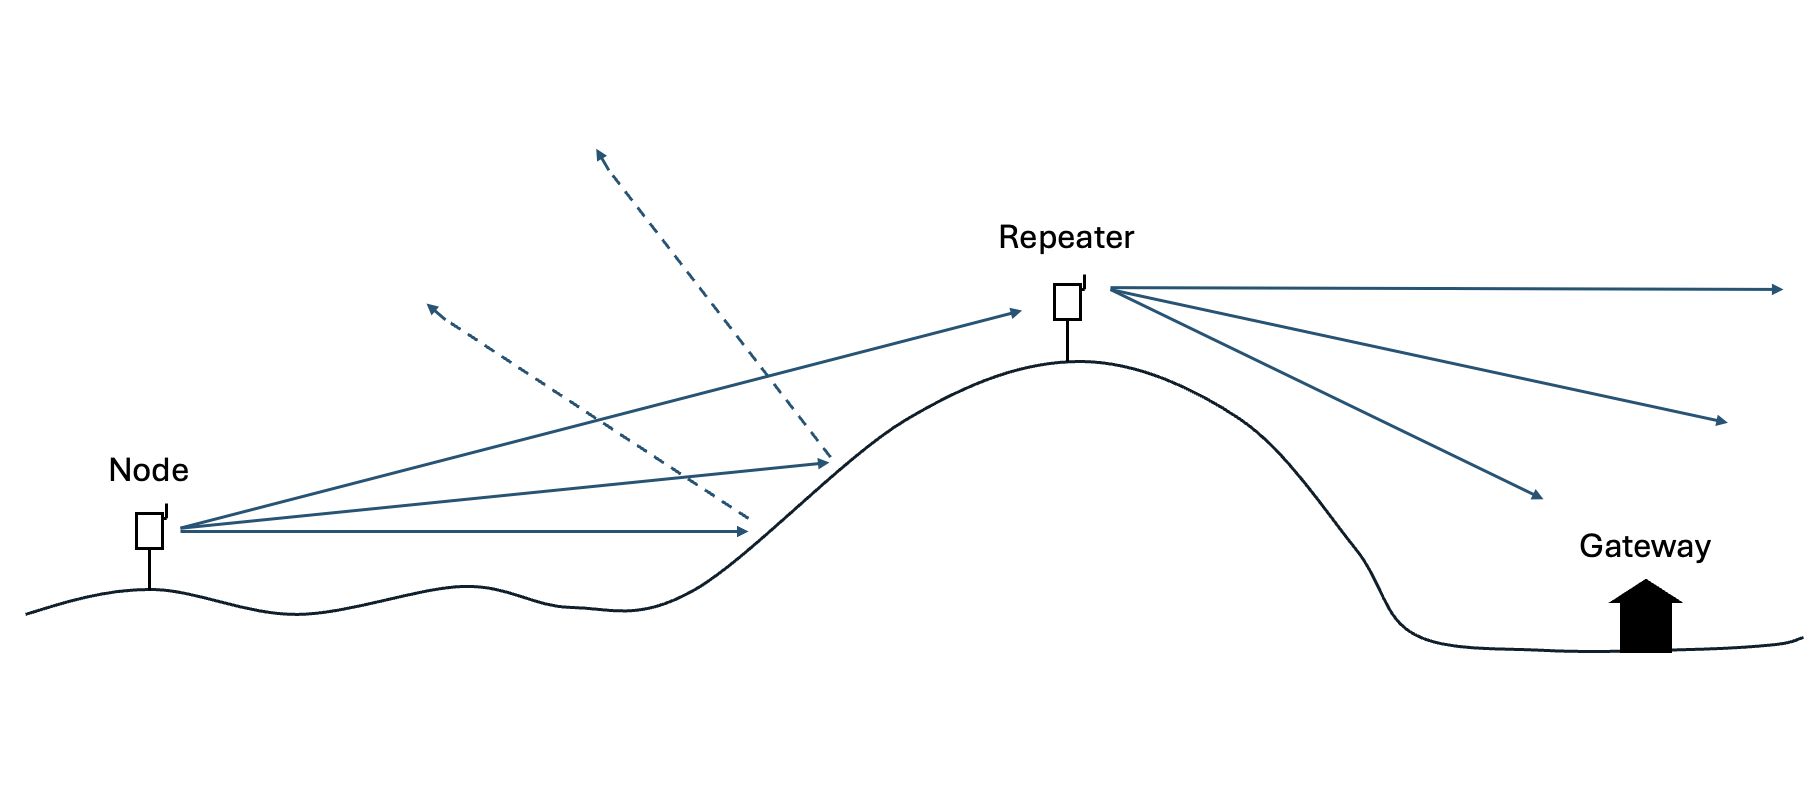
\includegraphics[width=0.9\textwidth]{contents/part-4/fig4/repeater.png}
  \caption{Illustration of LoRa radio propagation with a repeater included}
  \label{fig:repeater}
\end{figure}

\subsubsection{Reset behaviour}\label{sec:reset-behaviour}

As covered briefly in Chapter~\ref{sec:deployment}, the reset behaviour of the
Challenger is inconsistent after a brownout or complete power outage.
Essentially if the sensor nodes run out of power, there is no certainty that the
node will restart the code.py program when power returns. This is in spite of
the fact that I modified the safemode.py behaviour of CircuitPython with the
recommended code for remote solar power applications. As this ultimately appears
to be a firmware issue there is not an obvious or easy solution for this.

With enough time I would probably rewrite all of the Challenger software in
MicroPython and see if that firmware behaves in a more reliable and
deterministic way on power outage. Unfortunately the issue was picked up fairly
late in development and it was unrealistic to perform a refactor of this scale
with the time left.

\subsection{Quantitative comparison with commercial alternatives}

I will now compare the performance of my LoRa weather station to prebuilt
options available to purchase. A breakdown of costs for Agriscanner is included
in Appendix~\ref{app:cost-nodes}.

\begin{table}[H]
  \centering
  \small
  \renewcommand{\arraystretch}{1.2}
  \begin{tabularx}{\textwidth}{l >{\raggedright\arraybackslash}X
      >{\raggedright\arraybackslash}X >{\raggedright\arraybackslash}X
      >{\raggedright\arraybackslash}X >{\raggedright\arraybackslash}X}
    \hline
                                                    & \textbf{Agriscanner
    Network}                                        & \textbf{SenseCAP
    S2120\cite{pihut:sensecap-s2120-2025}}          & \textbf{Decentlab Eleven
    Parameter\cite{alliot:decentlab-eleven-2025}}   & \textbf{HOBO weather
    station kit\cite{weathershop:hobo-rx3000-2025}} & \textbf{SparkFun Arduino
    weather kit\cite{pihut:sparkfun-2025}} \\

    \hline
    Number of sensors                               & 4 & 8
    & 11\textsuperscript{*}                           & 6
    & 7                                \\
    Sensor accuracy                                 & Hobbyist & Hobbyist &
                                                    Professional & Professional
                                                    & Hobbyist \\
    Communication type                              & LoRa & LoRa & LoRa &
                                                    Mobile network        & WiFi
                                                    \\
    Update frequency                                & 1 minute & 1 hour & 10
                                                    minutes & 1 hour & 1 minute
                                                    \\
    Readings per hour                               & 60 & 1
    & 6                                               & 10
    & 60                               \\
    Power source included                           & Yes & Yes
    & Yes                                             & Yes
    & No                               \\
    Power source                                    & Solar & Solar & Solar &
                                                    Solar                 & --
                                                    \\
    Batteries recharge?                             & Yes & No
    & No                                              & Yes
    & --                               \\
    Reported battery life                           & replace $\sim$ 3 years &
    154 days                                        & Several months & replace
    3--5 years                                      & -- \\
    Reported range                                  & -- & 2--10\,km
    & 2--10\,km                                       & Anywhere with 4G & -- \\
    Estimated range                                 & 2.4--20\,km & 1.2--10\,km
                                                    & 1.2--10\,km & -- &
                                                    10--50\,m \\
    IP rating                                       & $\sim$ IP65 & IPX6 & IP66
                                                    & IP66                  &
                                                    None     \\
    Ongoing payment?                                & -- & --
    & --                                              & Yes -- mobile plan
    & -- \\
    Ongoing costs p.a                               & \pounds{}0 & \pounds{}0 &
                                                    \pounds{}0 & \pounds{}132 &
                                                    \pounds{}0 \\
    Cost per sensor node                            & \pounds{}177 &
    \pounds{}287                                    & \pounds{}3{,}272 &
    \pounds{}4{,}138                                & \pounds{}130 \\
    Cost per repeater                               & \pounds{}93 & \pounds{}0 &
                                                    \pounds{}0 & \pounds{}0 &
                                                    \pounds{}0 \\
    Cost per gateway\textsuperscript{**}            & \pounds{}66 & \pounds{}122
                                                    & \pounds{}122 & \pounds{}0
                                                    & \pounds{}0 \\
    Battery cost p.a.\textsuperscript{***}          & \pounds{}7 & \pounds{}10 &
                                                    \pounds{}30 & \pounds{}20 &
                                                    \pounds{}0 \\
    \textbf{Total cost\textsuperscript{****}}       & \textbf{\pounds{}520} &
    \textbf{\pounds{}706}                           & \textbf{\pounds{}6{,}696}
    & \textbf{\pounds{}8{,}418} & \textbf{\pounds{}260} \\
    \hline
  \end{tabularx}

  \vspace{0.25em}
  \textit{\footnotesize * Sensors missing from Agriscanner: Solar radiation,
    rainfall, barometric pressure, vapor pressure, dew point, wind direction,
    tilt sensor, lightning strike count / distance} \\
  \textit{\footnotesize ** For SenseCAP and Decentlab models the lowest cost
    gateway available is sensecap m2 at £122} \\
  \textit{\footnotesize *** Battery cost assumptions are detailed in
    Appendix~\ref{app:battery-assumptions}.} \\
  \textit{\footnotesize **** Includes sensors, repeater, gateway, and estimated first-year battery + ongoing costs.}
  \caption{Comparison of weather-station options.}
  \label{tab:commercial-comparison}
\end{table}

\subsubsection{Benefits of my weather station}

\begin{itemize}
  \item \textbf{Cost:} At £520\footnote{NB: The actual cost for this project is
        significantly lower as many components are being used on loan from the
        University of Bristol or purchased through my £150 dissertation
        allowance. The total charge to the DECIDE project is roughly £200. The
        larger figure here represents the value of components at market
        price.} the Agriscanner weather stations are the lowest cost option
        among waterproof, long-range systems. While the SparkFun kit is cheaper,
        it is not suitable for outdoor deployment due to its exposed electronics
        and, since it relies on WiFi, its range would be insufficient in an
        agricultural setting. It will therefore not be discussed further. The
        two professional systems (DecentLab and HOBO) are over ten times the
        price of my system and are therefore not comparable.

        The only system with similar characteristics under £1,000 that I could
        find is the SenseCAP device. However, with a cost per node roughly 50\%
        higher, my nodes still provide better value. If additional nodes were
        deployed, this price difference would become even more significant.

  \item \textbf{Frequency of readings:} My sensor nodes collect and transmit
        readings every minute, providing the Agriscanner webapp with effectively
        live data. By contrast, most alternative options only provide hourly
        readings, leaving actual conditions between measurements unknown.

  \item \textbf{Battery recharging:} My nodes use rechargeable 18650 batteries,
        which I conservatively estimate will last around three years (they use
        the same battery chemistry as mobile phones) before requiring
        replacement. Of the alternatives, only the HOBO system features a
        rechargeable battery. Both SenseCAP and DecentLab rely on disposable
        alkaline batteries, requiring regular replacement and therefore more
        frequent maintenance.

  \item \textbf{Range:} As explained in Section~\ref{sec:range-eval}, my weather
        station network benefits from the inclusion of a repeater. This enables
        significantly greater range than the other models could provide,
        particularly in hilly terrain.

        I also doubt whether either the SenseCAP or DecentLab systems could
        achieve a substantial range improvement under the same test conditions.
        In the UK, LoRa transmission power is subject to a strict regulatory cap
        (see Section~\ref{sec:lora-limit}). Since my system already operates at
        this maximum power, commercial products cannot exceed it. Even with a
        superior antenna, transmit power would need to be reduced
        proportionally, as antenna gain also counts towards the effective
        radiated power. It is therefore highly unlikely that these alternatives
        would achieve a range advantage sufficient to offset the benefits of a
        repeater in my system.
\end{itemize}

\subsubsection{Drawbacks of my weather station}

\begin{itemize}
  \item \textbf{Number of sensors:} One of the clearest drawbacks of the
        Agriscanner system is the lower sensor count: only four sensors compared
        with seven to eleven on competing systems. However, the Challenger
        microcontrollers in my sensor nodes still have spare GPIO ports, so
        adding additional sensors would be straightforward. The cost of many
        sensors is also not prohibitive (for example, a UV index sensor is only
        \pounds{}6).
  \item \textbf{Sensor accuracy:} Professional systems use higher-grade sensors
        with tighter accuracy specs. For example, the DecentLab unit specifies
        air temperature accuracy of $\pm0.6\,\si{\celsius}$, whereas the DHT11
        used in mine is only rated to about $\pm2.0\,\si{\celsius}$.
  \item \textbf{Reset behaviour:} As noted in Section~\ref{sec:reset-behaviour},
        the node firmware can behave unreliably after a full battery drain.
        While I cannot purchase the other devices in this list to confirm this
        directly, it is unlikely that the other units would exhibit the same
        behaviour, especially because their firmware will have been built
        specifically for remote solar powered applications.
  \item \textbf{Remote Health Diagnostics:} The Agriscanner provides no way to
        remotely monitor battery health and charging status. Such capabilities
        would help diagnose issues caused by poor choice of location for
        effective charging. A location that might have been acceptable at the
        time of installation might become non-viable as the sun becomes lower in
        the sky in the autumn and winter, or as vegetation grows and occludes
        the solar panels.
  \item \textbf{Other factors:} The other devices bring other non-tangible
        benefits besides their technical specification. For example, warranties,
        formal testing, vendor support etc. Professional systems commonly offer
        long-term maintenance and firmware updates beyond the initial purchase,
        which my prototype solution obviously does not offer.
\end{itemize}

\subsection{Conclusion on hardware performance}

While the weather station network has shown promising results as a low cost and
long range solution, the unreliable reset behaviour holds it back from being
100\% deployment ready. So far the weatherproofing of the external devices has
been encouraging, though testing has been limited due to unusually dry weather
and a longer deployment in wetter and colder conditions is needed. The outages
seen during the current deployment appear to be an issue specific to the private
garden they are in and would be much less likely in an open field environment;
however, this does emphasise the need for more extensive site surveys prior to
installation. Overall, if the reset behaviour can be addressed and a small
number of additional sensors are added, the complete system would be well suited
for long term unattended deployment on a farm.

\section{Web app: System Usability Survey}

Section will show results from SUS survey and conclude on strengths and what
could be improved about the web app in general. Also user stories for future
action that came out of the survey.

\subsection{Methodology}

\section{Machine learning model evaluation}

Section will compare machine learning models prediction to the actual sensor
data and the general forecast and conclude on whether model is appropriate for
application

\subsection{Methodology}



\section{Future work}\label{sec:future-work}

Ultimately the main objective of this work is to deploy the system in an apple
farm to assist the farmers with the management of their orchard. Before the
system can be deployed, the Challenger's firmware must be able to reliably
restart after a power outage.  As suggested in section \ref{sec:reset-behaviour}
I would first recommend experimenting with MicroPython to see if this can
provide a more robust solution to coping with this scenario. The worst case
scenario would be to have to use an alternative embedded processor that can
handle power fluctuations.

Additionally, it may be of value to add more sensor to the nodes as this is a
noticeable weakness of the current system architecture compared to existing
alternatives. Considering the addition of sensors would result in increased
power requirements I believe it would be inadvisable to add any more for time
being. Once the system has been deployed for an extended period and shows that
it can operate with minimal outages then the adding sensors would be a
worthwhile improvement to the current design.

Once the reliability issue has been resolved, the next stage will be to deploy
the system onto a farm.  The siting of the sensor nodes and repeater will need
careful consideration, so a thorough site survey should be undertaken prior to
this. It would be advisable to allow a few days for the installation, so there
is someone on hand to deal with any issues that might arise once the nodes have
been installed and to make sure the farmers are comfortable with using the
webapp.

I would recommend that the forecasting feature continues to be developed using
machine learning. Furthermore instead of training the model offline and manually
inserting models into the webapp, future work could focus on moving model
training online. This would allow the model to continually update and improve as
new data from the nodes is produced. After a few months of data is collected
then a repeated comparison should be performed to 


\section{Closing remarks}

This dissertation has shown the process of developing a complete IoT weather
station network with an accompanying webapp. In the hardware evaluation it was
shown that the system designed here offers superior range at lower cost. With
some extra time and effort put into fixing the reset behaviour the system has
demonstrated sufficient ruggedness to be deployed in field. 

The webapp designed here scored well in terms of usability, achieving a far
higher SUS score than the benchmark level of 68. The user stories developed from
survey responses also offers a clear roadmap to future development.

Finally the machine learning evaluation explored the accuracy of the current
machine learning system against a simpler model. With additional training data,
there should be a much higher degree of accuracy - and this was discussed as an
important area of future development. 


% References
\newpage
\addcontentsline{toc}{section}{References}
\printbibliography

\appendix
\newpage
\part{Appendices}

% Override spacing just for appendix
\makeatletter
\patchcmd{\section}{\clearpage\vspace*{3cm}\thispagestyle{plain}}{\clearpage\thispagestyle{plain}}{}{}
\titleformat{\part}[block]
{\normalfont\centering\bfseries} {\LARGE \partname\ \thepart}{1em}{\Huge}
[\thispagestyle{plain}\clearpage]
\makeatother
\newpage

%TC:ignore
\section{Breakdown of costs}\label{app:cost-nodes}

\begin{figure}[H]
    \centering
    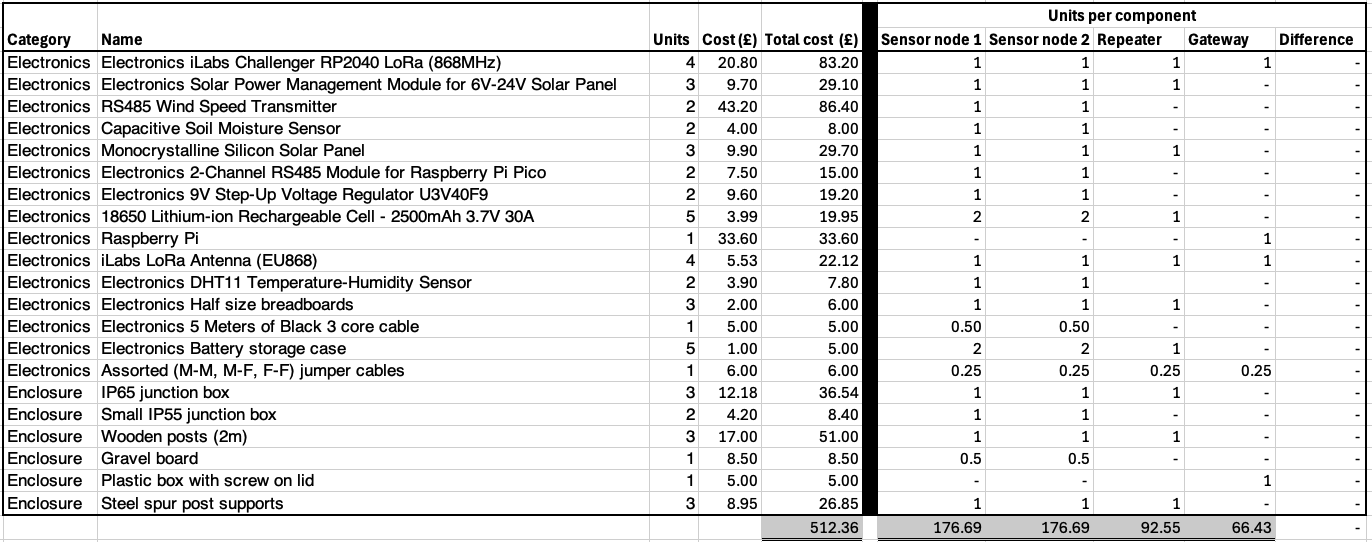
\includegraphics[width=1\textwidth]{contents/appendix/fig5/table.jpg}
    \caption{Table of component costs}
    \label{fig:cost-table}
\end{figure}

\begin{figure}[H]
    \centering
    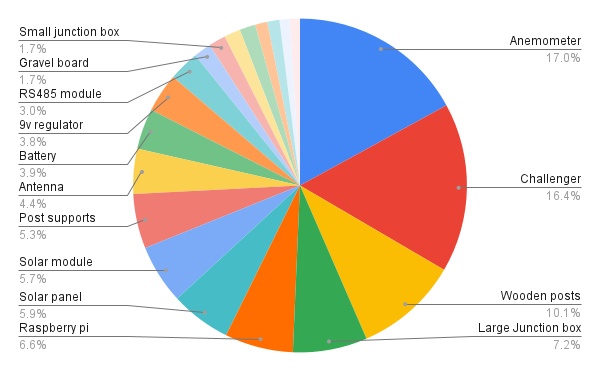
\includegraphics[width=0.8\textwidth]{contents/appendix/fig5/chart.png}
    \caption{Chart to visualise relative cost of components}
    \label{fig:cost-chart}
\end{figure}

\section{Interview excerpt with Small Brook Farms
owners}\label{sec:small-brook-interview}

Interviewer: So you would need a weather station to observe very local weather,
I expect. What you're saying is that the BBC website weather is not necessarily
relevant to you?

Speaker 1: No, No , so there's another site which is in Sanford and we can have
conversations - we're what? - 5 miles apart 10 miles? 

Speaker 2: Yeah. So the other side of that hill there like a mile away you get a
different sort of weather, but even on this side of the [apple orchard] as
opposed to that side of the [apple orchard] like the wind can be less than
whatever else, its very localised. But you know you if you then go on that side
of the valley, it doesn't rain on this side. So like to be actually useful,
yeah, [weather monitoring] sort of has to be [based on] the farm.

Source: Transcript no.28 of site visit from DECIDE sharepoint (9 May 2025)

\section{Battery cost assumptions}\label{app:battery-assumptions}
\begin{itemize}
  \item \textbf{Agriscanner Network:} Replace 5 (2 per sensor node, 1 for
  repeater) Li-ion batteries every 3 years at a cost of \pounds{}20
  \(\Rightarrow\) \(\approx\)\,\pounds{}7 per annum.
  \item \textbf{SenseCAP S2120:} Three AA batteries per node, replaced twice a
  year (total 12 batteries) \(\approx\)\,\pounds{}10 per annum.
  \item \textbf{Decentlab Eleven Parameter:} Two C batteries per node, replaced
  four times per year (total 16 batteries) \(\approx\)\,\pounds{}30 per annum.
  \item \textbf{HOBO weather station kit:} Replace lead-acid for each node
  battery every 4 years at a cost of \pounds{}80 \(\Rightarrow\)
  \(\approx\)\,\pounds{}20 per annum.
\end{itemize}

\section{System usability survey}\label{app:sus-survey}

\begin{figure}[H]
    \centering
    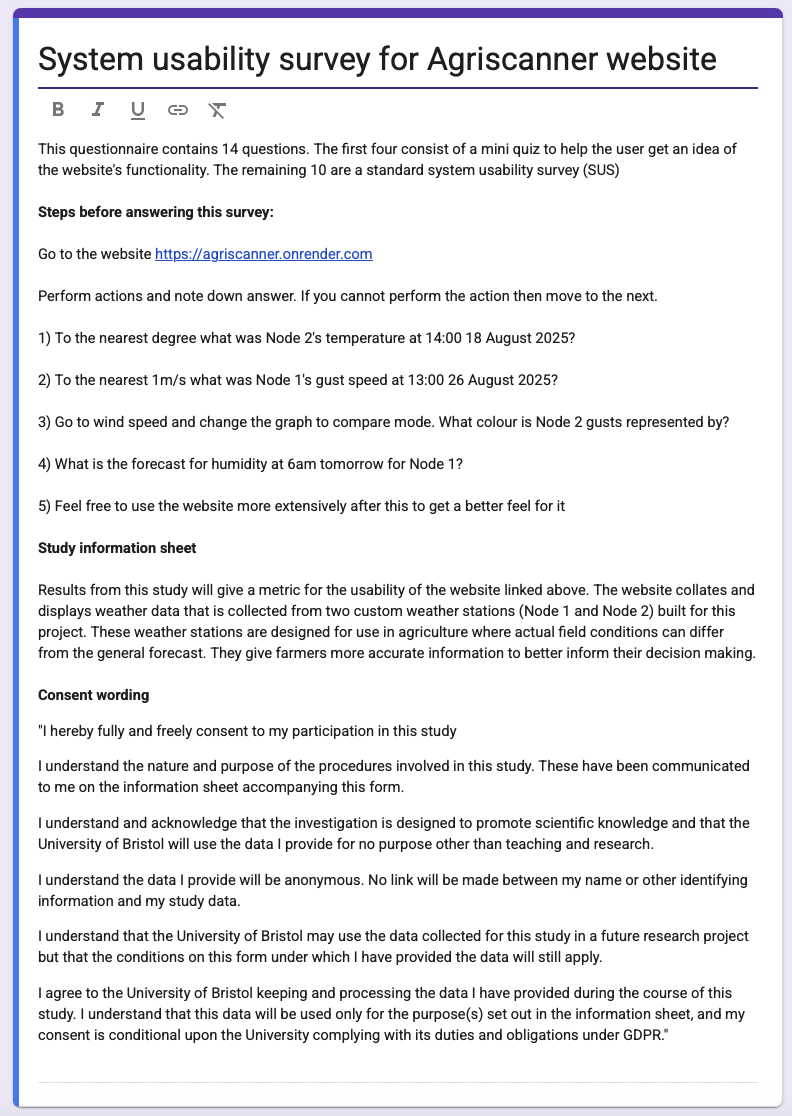
\includegraphics[width=0.9\textwidth]{contents/appendix/fig5/sus_survey.png}
    \caption{SUS survey wording}
    \label{fig:survey-wording}
\end{figure}

List of tasks for users:

\begin{enumerate}\label{list-of-tasks}
  \item To the nearest degree, what was Node 2's temperature at 14:00 18 August
  2025?
  \item To the nearest 1\,m/s, what was Node 1's gust speed at 13:00 26 August
  2025?
  \item Go to wind speed and change the graph to compare mode. What colour is
  Node 2 gusts represented by?
  \item What is the forecast for humidity at 06:00 tomorrow for Node 1?
\end{enumerate}

\section{Additional SUS materials}\label{app:correlation-sus}

\begin{figure}[H]
    \centering
    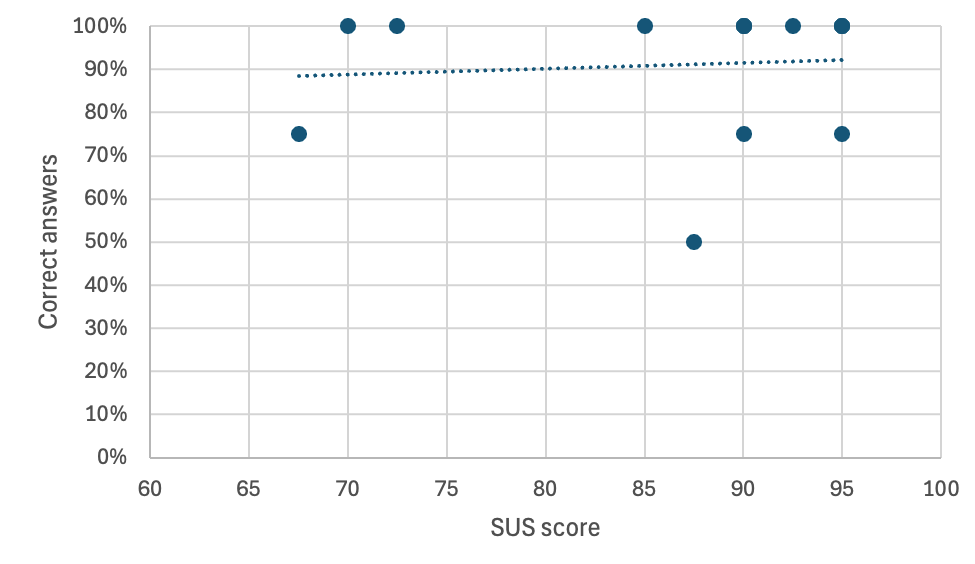
\includegraphics[width=0.9\textwidth]{contents/appendix/fig5/answer-sus-correlation.png}
    \caption{Graph to show SUS score vs percent of correct answers ($R^2 = 0.0066$)}
    \label{fig:sus-correlation}
\end{figure}

\begin{table}[ht]
  \centering
  \begin{tabular}{r r r r}
    \hline
    responder\_num & sus\_score & correct\_answers & type\\
    \hline
    1  &  90.0  & 75\%  & desktop\\
    2  &  92.5  & 100\% & mobile\\
    3  &  95.0  & 100\% & mobile\\
    4  &  70.0  & 100\% & desktop\\
    5  &  90.0  & 100\% & mobile\\
    6  &  90.0  & 100\% & desktop\\
    7  &  87.5  & 50\%  & desktop\\
    8  &  95.0  & 100\% & mobile\\
    9  &  95.0  & 75\%  & mobile\\
    10 &  95.0  & 100\% & desktop\\
    11 &  72.5  & 100\% & desktop\\
    12 &  67.5  & 75\%  & mobile\\
    13 & 100.0  & 100\% & mobile\\
    14 &  90.0  & 100\% & mobile\\
    15 &  85.0  & 100\% & desktop\\
    \hline
  \end{tabular}
  \caption{Raw SUS scores and correct answer percentage from survey}
  \label{tab:raw-sus}
\end{table}

% Requires: \usepackage{float} Also requires: \usepackage{amsmath}
\begin{figure}[H]
  \centering
  \begin{minipage}{0.9\textwidth}
    \begin{quote}
    ``I found it very hard to get to a specific time on the graph - the
    granularity of the cursor moving seemed to make it hard to choose my time -
    I ended up with 14:01 for the first question as I couldn't get the cursor to
    stay at 14:00. But as a weather nerd I loved it.''
    \end{quote}
 \vspace{8pt}
    \begin{quote}
    ``I found it annoying having to click to get to the required date. Also I
    don't understand from the website alone what the project is about or where
    the data is from - maybe an about page would be nice :)''
    \end{quote}
 \vspace{8pt}
    \begin{quote}
    ``Sorry wasn’t sure where the compare graph is but the website looked really
    nice!''
    \end{quote}
  \end{minipage}
  \caption{Feedback from participants with lower SUS scores}
  \label{fig:low-sus-feedback}
\end{figure}

\begin{figure}[H]
  \centering
  \begin{minipage}{0.9\textwidth}
    \begin{quote}
    "The soil moisture readings surprised me - I expected them to go up with
    rain (increased moisture) but they went down.  I think this is
    counter-intuitive and there should either be some explanation of the what
    the measurements mean, or preferably there should be an option to convert to
    a more human understandable description like very dry/dry/slightly
    moist.../wet/very wet/saturated"
    \end{quote}
 \vspace{8pt}
    \begin{quote}
    "When selecting the date (specifically when clicking the arrows to move
    forwards and backwards in time) it would be useful to have a calendar
    display to travel to past dates quicker."
    \end{quote}
 \vspace{8pt}
    \begin{quote}
    "Extra features: - Date picker instead of having to navigate past each day -
    Export feature to export data in bulk (e.g. to a csv) - Ability to select a
    time period (specific dates) instead of just a day view"
    \end{quote}
 \vspace{8pt}
    \begin{quote}
    "I think when switching dates, it should support selecting a date from the
    calendar rather than only moving forward or backward to the nearest dates."
    \end{quote}
 \vspace{8pt}
    \begin{quote}
    "Being able to navigate directly between measurements (e.g. temp, humidity
    etc.) while on [sic]"
    \end{quote}
 \vspace{8pt}
    \begin{quote}
    "Finding the "compare" option was the hardest part. But didn't take long." 
    \end{quote}
 \vspace{8pt}
    \begin{quote}
    "Great website- simple layout and easy to use!"
    \end{quote}
 \vspace{8pt}
    \begin{quote}
    "No bugs seen, but on wind graph some of the y axis text was slightly cut
    off on my screen. I'm on a laptop"
    \end{quote}
  \end{minipage}
  \caption{Feedback from participants with higher SUS scores}
  \label{fig:high-sus-feedback}
\end{figure}

\begin{figure}[H]
  \makebox[\textwidth][r]{ \fbox{
      \begin{minipage}[c][8cm][c]{0.85\textwidth}
        \raggedright

        Both the Mann Whitney U and Wilcoxon Signed Rank test were selected for
        this data because the SUS score is derived from Likert items. Likert
        items are ordinal (e.g. strongly disagree) and so nonparametric
        statistical testing is typically preferred
        \cite{bobbitt_mann-whitney_2022}\vspace{8pt}

    The Mann Whitney U statistical test score was calculated in an Excel sheet I
    made using the procedure described in \cite{bobbitt_mann-whitney_2022} and
    the result cross-verified using the website in \cite{socscistats} which is
    also the source of the p-value. Results: U = 13.5, critical value = 10
    p=0.10524. Parameters: two-tailed, 0.05 significance\vspace{8pt}
    
    Due to the complexity of calculating it, the one-sample Wilcoxon Signed Rank
    Test score was calculated in Excel using a modified template from the source
    in \cite{peterstatistics_wilcoxon_2025} and cross-verified with the website
    in \cite{statsBlue}. Results: \(W^{+}=119\) z = 3.3361, critical value =
    1.6449 Parameters: right-tailed, 0.05 significance \end{minipage} } }
  \caption{Note on statistical testing}
  \label{fig:appendix-note-1}
\end{figure}

% \section{Nielsen's nine usability heuristics
% \cite{nielsen1990heuristic}}\label{app:usability-heuristics}

% \begin{itemize} \item Simple and natural dialogue \item Speak the user's
%   language \item Minimize user memory load \item Be consistent \item Provide
%   feedback \item Provide clearly marked exits \item Provide shortcuts \item
%   Good error messages \item Prevent errors \end{itemize}


\section{How LoRa works}\label{app:lora-explained}

As this paper is not a technical study of radio communication I will opt for a
brief summary of the principles behind LoRa. With this in mind I have based much
of the information from the excellent video lecture in \cite{visualelectric2021}
that itself draws upon the paper in \cite{vangelista2017}.

The reason LoRa modulation is different to traditional modulation techniques is
the use of a "chirp" as the key to transmitting packets. A more traditional
technique might involve a frequency shift key; that is a single frequency
represents several bits. These unique frequencies are called symbols as they
represent data, like letters in the alphabet. In the below graph we see three
simplified symbols that represent binary values, the combination of these
symbols makes a packet:

\begin{figure}[H]
  \centering
  % left image
  \begin{minipage}{0.48\textwidth}
    \centering
    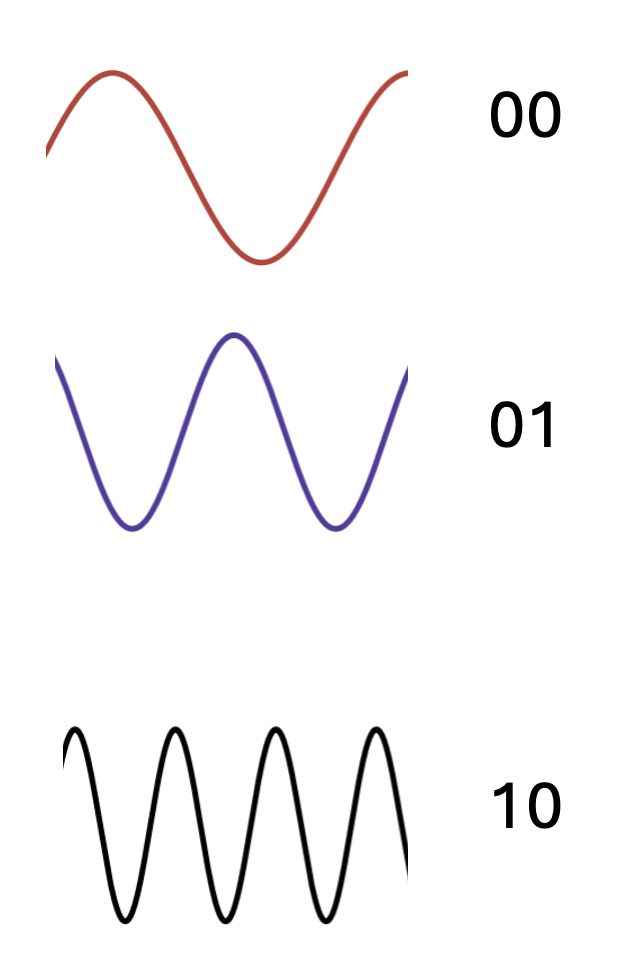
\includegraphics[width=0.4\linewidth]{contents/part-1/fig1/frequencysymbols.png}
    \\[4pt]
    {\small (a) Frequency shift symbols} \end{minipage}\hfill
  % right image
  \begin{minipage}{0.48\textwidth}
    \centering
    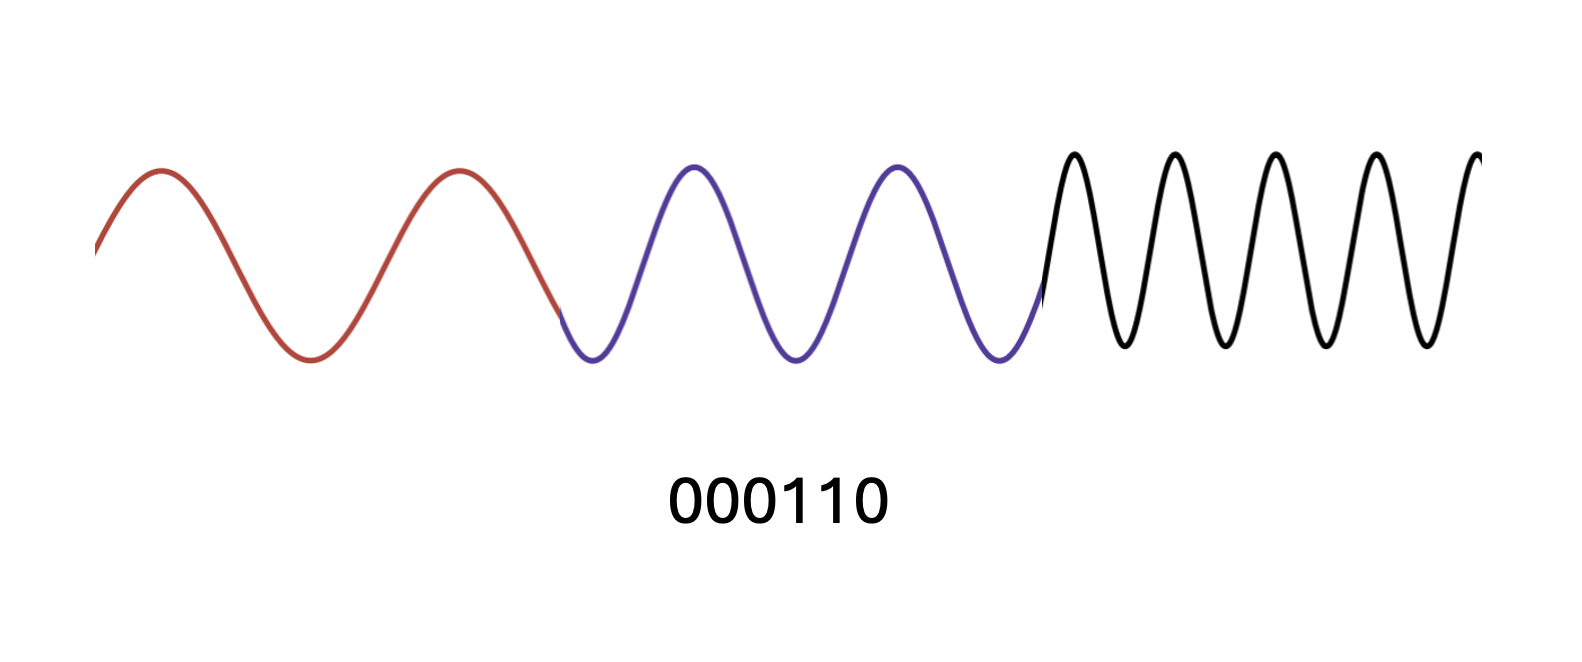
\includegraphics[width=1\linewidth]{contents/part-1/fig1/packet.png}
    \\[4pt]
    {\small (b) Packet}
  \end{minipage}
  \caption{ Traditional radio modulation with frequency symbols}
  \label{fig:freq-and-packet}
\end{figure}

In traditional modulation, symbols always have flat unchanging frequency (as can
be seen from the fact the wave separation never changes). LoRa symbols instead
have changing frequencies that have a waveform like the below.

\begin{figure}[H]
    \centering
    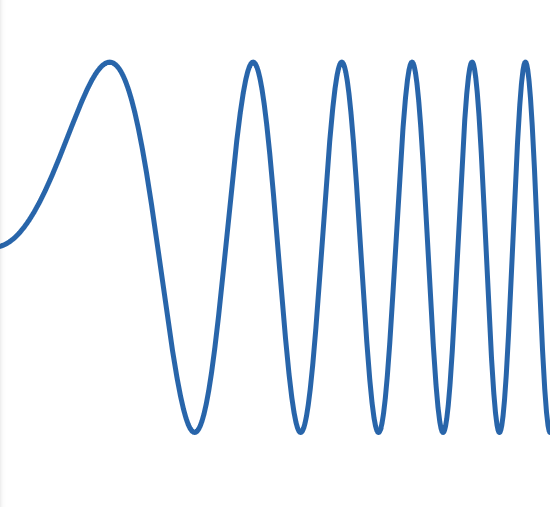
\includegraphics[width=0.15\textwidth]{contents/part-1/fig1/lorawavelength.png}
    \caption{LoRa symbol showing changing frequency ("Up-chirp")}
    \label{fig:lora-wave}
\end{figure}

This change in frequency is what gives the wave form the name "chirp". If
traditional frequency symbols were thought of a sound they would be similar to
morse code beeps while LoRa would be more similar to siren or \textit{chirp}ing
bird. LoRa has both rising and falling chirps (up-chirps and down-chirps).

Different LoRa symbols are then distinguished by the point in time of a
discontinuity. LoRa symbols are always delivered over a known length of time, so
different symbols include a reset back to the starting frequency at a different
point in time.

A way to graphically show this discontinuity in LoRa and compare it to frequency
shift modulation is by using instantaneous frequency graphs:

\begin{figure}[H]
  \centering
  % left image
  \begin{minipage}{0.48\textwidth}
    \centering
    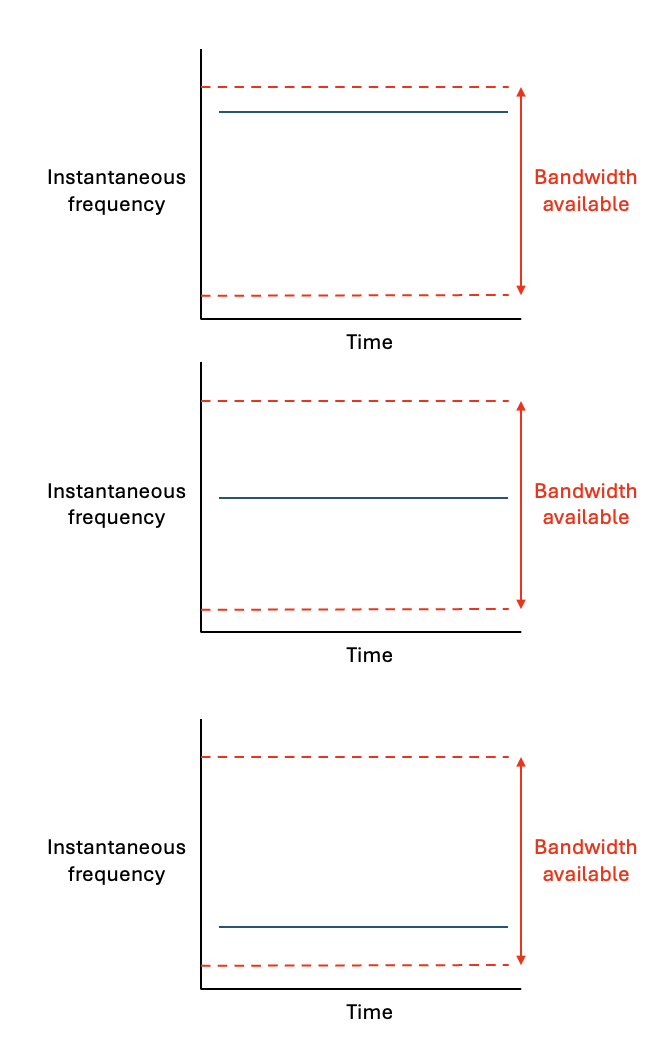
\includegraphics[width=0.9\linewidth]{contents/part-1/fig1/traditional-wavechart.png}
    \\[4pt]
    {\small (a) Frequency shift symbols} \end{minipage}\hfill
  % right image
  \begin{minipage}{0.48\textwidth}
    \centering
    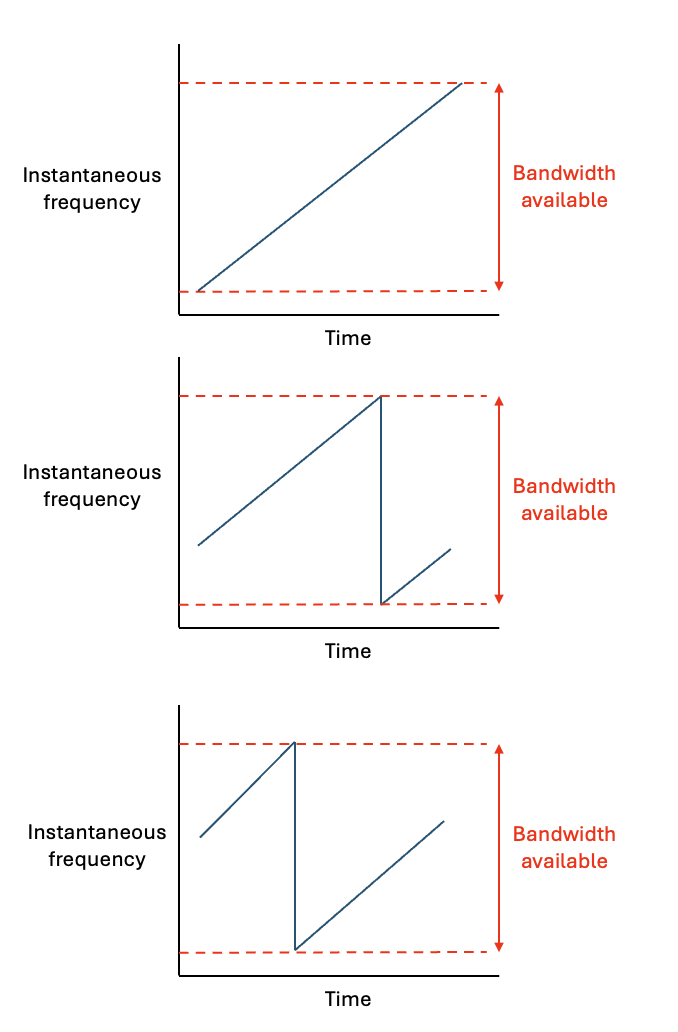
\includegraphics[width=0.9\linewidth]{contents/part-1/fig1/lora-wavechart.png}
    \\[4pt]
    {\small (b) LoRa symbols, note shifting discontinuity}
  \end{minipage}
  \caption{ Comparison of frequency shift and LoRa modulation }
  \label{fig:freq-vs-lora}
\end{figure}

Once these symbols hit the receiver, the receiver must work out which symbol it
was. In frequency shift modulation this is achieved by performing a correlation
test against every symbol received. However this is computationally difficult
and requires a low signal-to-noise ratio to work effectively. The benefit of
chirps is that due to a mathematical transformation that will not be further
discussed (Fast Fourier transform), the correlation can be computed much more
easily and with less powerful hardware.


\section{IoT enabling technologies} \label{app:enabling-tech}

This supplementary section lists the key technological developments that have
are contributed to the viability of my project.

\begin{enumerate}
  \item Efficiency improvements in microchips - breakthroughs in microchip
  fabrication have led to smaller more efficient chips with improved
  performance.
  \item Lithium-Ion batteries improvements - continuous improvements in the
  energy density of lithium-ion batteries has made it possible to power devices
  for long periods without mains power.
  \item Low-power long-range radio - new radio communication techniques such as
  LoRa allow for data transmission over several kilometres using a fraction of
  the power required by traditional mobile or Wi-Fi technologies.
  \item Affordability of solar panels - since 1970 the price of solar panels has
  decreased to 1/500th of its original cost \cite{economist2024} making solar a
  viable power source for IoT systems.
  \item Growth of hobbyist embedded systems - since the release of accessible
  platforms such as Arduino in 2005, the growth of hobby level embedded systems
  has lowered the barrier to entry to create IoT systems.
  \item Accessible cloud computing and hosting - Cheap and available web hosting
  has allowed application level systems to be more easily developed.
\end{enumerate}

\section{CircuitPython sensor node 1 code example}\label{app:sensor-code}

\begin{multicols}{2}
\begin{lstlisting}
#Code adapted from iLabs example by Jerry Needle 2021 (the LoRa setup)

import time
import board
import busio
import digitalio
import adafruit_rfm9x
import adafruit_dht
import analogio


DEVICE_ID = 1
RADIO_FREQ_MHZ = 868.0
WIND_REQUEST = bytes([0x02, 0x03, 0x00, 0x00, 0x00, 0x01, 0x84, 0x39])

# Initialise LORA radio and settings
try:
    spi = busio.SPI(board.RFM95W_SCK, MOSI=board.RFM95W_SDO, MISO=board.RFM95W_SDI)
    cs  = digitalio.DigitalInOut(board.RFM95W_CS)
    rst = digitalio.DigitalInOut(board.RFM95W_RST)
    rfm9x = adafruit_rfm9x.RFM9x(spi, cs, rst, RADIO_FREQ_MHZ)

    rfm9x.tx_power = 13
    rfm9x.spreading_factor = 7
    rfm9x.signal_bandwidth = 125_000
    rfm9x.coding_rate      = 5
    rfm9x.enable_crc       = True
    rfm9x.implicit         = False

except Exception as e:
    rfm9x = None
    print("ERR: Lora module", e)
    
# Initialise UART and settings    
try:
    uart = busio.UART(tx=board.GP16, rx=board.GP17, baudrate=9600, timeout=0.2)
except Exception as e:
    uart = None
    print("ERR: UART", e)
    
# Initialise the soil moisture sensor    
try:    
    moisture_pin = analogio.AnalogIn(board.A0)
except Exception as e:
    moisture_pin = None
    print("ERR: moisture pin", e)

# Initialise DHT11 temperature humidity sensor
try:
    dht_device = adafruit_dht.DHT11(board.A1)
except Exception as e:
    dht_device = None
    print("ERR: dht11", e)
    
# Returns raw soil moisture reading
def get_raw_moisture(pin):
    try:
        raw = pin.value   
        return raw
    except:
        return None

# Returns wind speed sensor using MODBUS protocol
def get_wind_speed():
    if uart:
        try:
            uart.write(WIND_REQUEST)
            time.sleep(0.2)
            response = uart.read(16)
            if response:
                if len(response) >= 5 and response[0] == 0x02 and response[1] == 0x03:
                    value_raw = response[3] << 8 | response[4]
                    return value_raw / 10.0
                else:
                    print("Bad format error")
                    return None
            else:
                print("No response error")
                return None
        except:
            print("Unknown error")
            return None
    print("Bad UART error")
    return None

def find_err(value):
    if value is None:
        return "ERR"
    else:
        return value

counter = 0

while True:
    
    t_sum = h_sum = w_sum = 0.0
    s_sum = 0
    t_n = h_n = s_n = w_n = 0
    min_counter = 0
    w_max = 0
    
    # Do 10 readings each minute and then average the minute result
    # If an exception occurs use pass to keep running
    while min_counter < 10:
        if dht_device:
            try:
                t_reading = dht_device.temperature
                if t_reading is not None:
                    t_sum += float(t_reading)
                    t_n += 1
            except Exception:
                pass
            try:
                h_reading = dht_device.humidity
                if h_reading is not None:
                    h_sum += float(h_reading)
                    h_n += 1
            except Exception:
                pass
        s_reading = get_raw_moisture(moisture_pin)
        
        if s_reading is not None:
            s_sum += s_reading
            s_n += 1
            
        w_reading = get_wind_speed()
        
        if w_reading is not None:
            w_sum += float(w_reading)
            w_n += 1
            if w_reading > w_max:
                w_max = w_reading
        print(f"{t_reading}, {h_reading}, {s_reading}, {w_reading}")
        min_counter += 1
        time.sleep(6)
        
        
    if t_n != 0:    
        t_avg = round(t_sum/t_n, 1)
    else:
        t_avg = None
    if h_n != 0:    
        h_avg = int(round(h_sum/h_n, 1))
    else:
        h_avg = None
    if s_n != 0:    
        s_avg = int(round(s_sum/s_n, 0))
    else:
        s_avg = None
    if w_n != 0:
        w_avg = round(w_sum/w_n, 1)
    else:
        w_avg = None
        w_max = None
    
    #send payload and include errors if found
    payload = f"{DEVICE_ID},{find_err(t_avg)},{find_err(h_avg)},{find_err(s_avg)},{find_err(w_avg)}, {find_err(w_max)},{counter}"
    try:
        rfm9x.send(payload.encode("utf-8"))
        print(f"Sent packet {payload}")
    #If sending the payload fails then print error
    except Exception as e:
        print("Failed to send packet: ", e)

    counter += 1
\end{lstlisting}
\end{multicols}

\section{Typescript API endpoint code for node data
insert}\label{app:api-endpoint}
\begin{multicols}{2}
\begin{lstlisting}
// End point to insert into node_data table
app.post('/api/database/insert-node-data', async (req: Request, res: Response) => {
  //Assign JSON body variables
  const {
    device_id,
    packet_id,
    temperature,
    humidity,
    soil_moisture,
    wind_speed,
    gust_speed,
    rssi0,
    rssi1,
    snr0,
    snr1,
  } = req.body;

  //attempt an insert with values from the json body
  try {
    const query = `INSERT INTO node_data 
      (node_deployment_id, farm_id, packet_id, temperature, humidity, 
      soil_moisture, wind_speed, gust_speed, rssi0, rssi1, snr0, snr1, node_name)
      VALUES (
      (SELECT id FROM node_deployment WHERE node_name = $11 ORDER BY ts DESC LIMIT 1),
      (SELECT farm_id FROM node_deployment WHERE node_name = $11 ORDER BY ts DESC LIMIT 1),
      $1,$2,$3,$4,$5,$6,$7,$8,$9,$10,$11);`;
    const values = [
      packet_id,
      temperature,
      humidity,
      soil_moisture,
      wind_speed,
      gust_speed,
      rssi0,
      rssi1,
      snr0,
      snr1,
      device_id
    ];
    //put query into pooled connection
    await pool.query(query, values);
    //return success if successful
    res.status(200).json({ status: 'success' });
  } catch (error) {
    console.error(error);
    //return error if error occurs in insert
    res.status(500).json({ error: 'failed to insert to database' });
  }
});

\end{lstlisting}
\end{multicols}

\section{Python code to train machine learning model}\label{app:ml-code}
\begin{multicols}{2}
\begin{lstlisting}
import pandas as pd
import numpy as np
import lightgbm as lgb
import joblib as jl
import m2cgen as m2c
from sklearn.metrics import mean_absolute_error, mean_squared_error

VALIDATION_PERCENT = 0.2
NODE_ID = 1
TARGET = 'temperature'

NODE_PREFIX = 'node_' + f'{NODE_ID}'
TARGET_COL = NODE_PREFIX + '_' + TARGET

# Read the csv and make it into pandas dataframe
data_frame = pd.DataFrame(pd.read_csv(NODE_PREFIX + '_training_data.csv'))

# Remove sensor data other than the target
cols_to_remove = ['ts']
for col in data_frame.columns:
    col_name = str(col)
    if col_name != TARGET_COL and col_name.startswith(NODE_PREFIX):
        cols_to_remove.append(col_name)

data_frame = data_frame.drop(columns = cols_to_remove)

# Set the split for training and validation data
cut_off_index = int(round((1- VALIDATION_PERCENT) * len(data_frame), 0))

# Define the data 
training_data = data_frame.iloc[:cut_off_index]
validation_data = data_frame.iloc[cut_off_index:]

# Define the features used for prediction
features = ['day_sin', 'day_cos', 'year_sin', 'year_cos', 'temp', 'pressure', 
'humidity', 'uvi', 'clouds', 'wind_speed', 'wind_gust', 'rain_1h', 'snow_1h']

# Initialise LGBM with following parameters
training_model = lgb.LGBMRegressor(
    n_estimators=250, 
    learning_rate=0.05
)

# Fit the model using features and target data 
training_model.fit(
    training_data[features],
    training_data[TARGET_COL],
    eval_metric='rmse',
    eval_set=[(validation_data[features], validation_data[TARGET_COL])],
    # Stop running training after 50 iterations of no improvement
    callbacks=[lgb.early_stopping(50), lgb.log_evaluation(20)]
)

# If it ends from best iteration get the date from this
best_iteration = getattr(training_model, "best_iteration_", None)
if best_iteration:
    prediction = training_model.predict(validation_data[features], num_iteration=best_iteration) 
else:
    training_model.predict(validation_data[features])

#Console log useful stats
print("Mean absolute error:", mean_absolute_error(validation_data[TARGET_COL], prediction))
print("Root mean squared error:", np.sqrt(mean_squared_error(validation_data[TARGET_COL], prediction)))
print("Features used:", training_model.booster_.feature_name())

#Export final model to JS
javascript_final_model = m2c.export_to_javascript(training_model)

with open(f'{TARGET}{NODE_ID}.js', 'w') as f:
    f.write(javascript_final_model)

    \end{lstlisting}
\end{multicols}

\section{Mean absolute error (MAE) and root mean squared error (RMSE) from
forecast comparison}\label{app:ml-stats}

\begin{figure}[H]
    \centering
    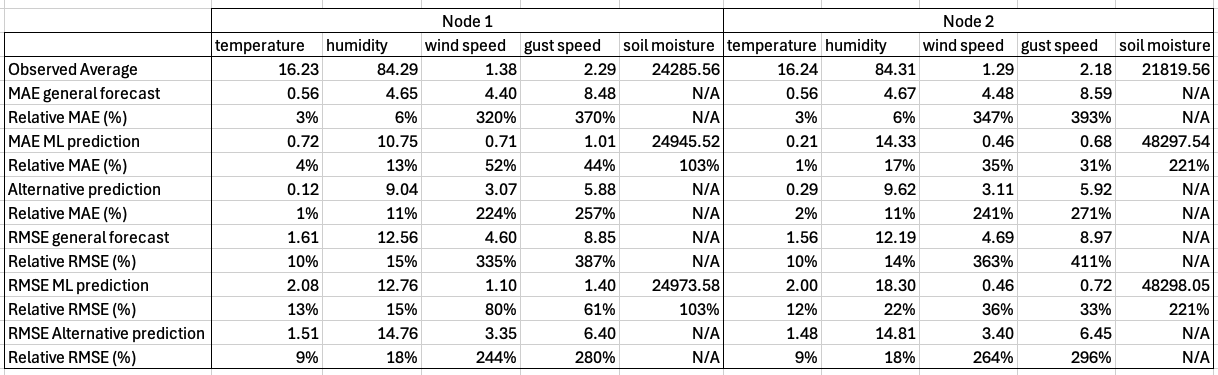
\includegraphics[width=0.9\textwidth]{contents/appendix/fig5/mae-rmse.png}
    \caption{General forecast is OpenWeather, Machine learning refers to my models, alternative refers to a mean adjusted general forecast model}
    \label{fig:mae-rmse}
\end{figure}

\begin{figure}[H]
    \centering
    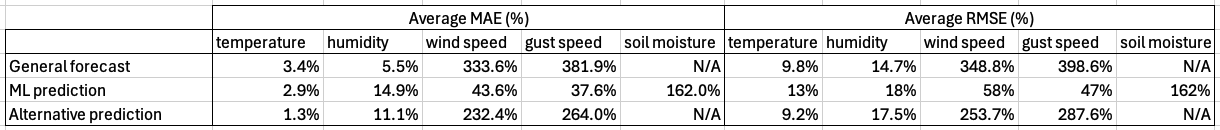
\includegraphics[width=1\textwidth]{contents/appendix/fig5/rel-mae-rmse.png}
    \caption{Table with relative MAE and RMSE averaged across node 1 and 2}
    \label{fig:rel-mae-rmse}
\end{figure}

\section{Alternative model data}\label{app:alt-data}

The below figure was used to produce the alternative model by applying these
adjustments to the general OpenWeather forecast. A positive reading means sensor
data was higher than forecast.

\begin{figure}[H]
    \centering
    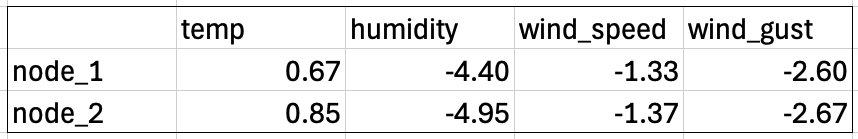
\includegraphics[width=1\textwidth]{contents/appendix/fig5/average-difference.png}
    \caption{Spreadsheet snippet showing average difference between general forecast and sensor readings between (15-27 August)}
    \label{fig:alt-data-ig}
\end{figure} 
%TC:endignore

\end{document}
